

% ============================================================================
% SECTION 1: TITLE PAGE & PRELIMINARY (Abjad numbering)
% ============================================================================

% !TEX root = main.tex
% ============================================================================
% TITLE PAGE
% ============================================================================

\begin{titlepage}


@@CENTER_START@@


    
\includegraphics[width=3cm]{iau_logo} \\
    \vspace{0.5cm}
    \textbf{\Large دانشگاه آزاد اسلامی واحد بندرعباس} \\
    \textbf{\large دانشکده مهندسی کامپیوتر و فناوری اطلاعات} \\
    \vspace{1.5cm}
    \textbf{\huge پایان‌نامه برای دریافت درجه کارشناسی ارشد در رشته مهندسی کامپیوتر} \\
    \vspace{0.5cm}
    \textbf{\Large گرایش نرم‌افزار} \\
    \vspace{1.5cm}
    \textbf{\huge رمزنگاری تصاویر رنگی با استفاده از ترکیب سیستم‌های آشوبناک مبتنی بر سیستم آشوب نمایی} \\
    \vspace{2cm}
    \textbf{\Large نگارش:} \\
    \textbf{\Large منصور زاهدی} \\
    \vspace{1cm}
    \textbf{\Large استاد راهنما:} \\
    \textbf{\Large دکتر حبیب خدادادی} \\
    \vspace{0.8cm}
    \textbf{\Large استاد مشاور:} \\
    \textbf{\Large مهندس بهارک احمدی پور} \\
    \vfill
    \textbf{\Large ۱۴۰۵ (تابستان)}


@@CENTER_END@@


\end{titlepage}


@@PB@@


\setcounter{page}{2}

% ============================================================================
% BISMILLAH PAGE
% ============================================================================
\thispagestyle{empty}


@@CENTER_START@@


    \vspace*{\fill}
    
\includegraphics[width=0.55\textwidth,keepaspectratio]{images/besmellah.png}
    \vspace*{\fill}


@@CENTER_END@@




@@PB@@


      % ا (الف)
\chapter*{صورت‌جلسه دفاع از پایان‌نامه}

بدین‌وسیله گواهی می‌شود که پایان‌نامه کارشناسی‌ارشد آقای \textbf{منصور زاهدی} با عنوان:


@@CENTER_START@@


\textbf{«رمزنگاری تصاویر رنگی با استفاده از ترکیب سیستم‌های آشوبناک مبتنی بر سیستم آشوب نمایی»}


@@CENTER_END@@


در تاریخ ......................... توسط هیئت داوران مورد بررسی و ارزیابی قرار گرفت و با درجه ......................... و نمره ......................... مورد تصویب نهایی قرار گرفت.

\vspace{2cm}



@@CENTER_START@@


\begin{tabular}{ccc}
\textbf{نام و نام خانوادگی} & \textbf{سمت} & \textbf{امضا} \\ \hline
......................... & استاد راهنما & ......................... \\
......................... & استاد داور داخلی & ......................... \\
......................... & استاد داور خارجی & ......................... \\
......................... & مدیر گروه & ......................... \\
\end{tabular}


@@CENTER_END@@





@@PB@@

          % ب (Jury approval)
\chapter*{تعهدنامه اصالت رساله یا پایان‌نامه تحصیلی}

اینجانب \textbf{منصور زاهدی} دانش‌آموخته مقطع کارشناسی‌ارشد در رشته \textbf{مهندسی کامپیوتر - نرم‌افزار} که در تاریخ ......................... از پایان‌نامه خود تحت عنوان:


@@CENTER_START@@


\textbf{«رمزنگاری تصاویر رنگی با استفاده از ترکیب سیستم‌های آشوبناک مبتنی بر سیستم آشوب نمایی»}


@@CENTER_END@@


با کسب نمره ............. و درجه ............................. دفاع نموده‌ام، بدین‌وسیله متعهد می‌شوم:

\begin{enumerate}
    \item این پایان‌نامه حاصل تحقیق و پژوهش انجام‌شده توسط اینجانب بوده و در مواردی که از دستاوردهای علمی و پژوهشی دیگران (اعم از پایان‌نامه، کتاب، مقاله و ...) استفاده نموده‌ام، مطابق ضوابط و رویه موجود، نام منبع مورد استفاده و سایر مشخصات آن را در فهرست مربوطه ذکر و درج کرده‌ام.
    \item این پایان‌نامه قبلاً برای دریافت هیچ مدرک تحصیلی (هم‌سطح، پایین‌تر یا بالاتر) در سایر دانشگاه‌ها و مؤسسات آموزش عالی ارائه نشده است.
    \item چنانچه بعد از فراغت از تحصیل، قصد استفاده و هرگونه بهره‌برداری اعم از چاپ کتاب، ثبت اختراع و ... از این پایان‌نامه داشته باشم، از حوزه معاونت پژوهشی واحد مجوزهای مربوطه را اخذ نمایم.
    \item چنانچه در هر مقطع زمانی خلاف موارد فوق ثابت شود، عواقب ناشی از آن را می‌پذیرم و دانشگاه آزاد اسلامی واحد بندرعباس مجاز است با اینجانب مطابق ضوابط و مقررات رفتار نموده و در صورت ابطال مدرک تحصیلی‌ام، هیچ‌گونه ادعایی نخواهم داشت.
\end{enumerate}

\vspace{1cm}

\begin{flushleft}
\begin{tabular}{l}
\textbf{نام و نام خانوادگی دانشجو:} منصور زاهدی \\
\textbf{تاریخ:} ......................... \\
\textbf{امضا:} ......................... \\
\end{tabular}
\end{flushleft}



@@PB@@

   % ج (Authenticity undertaking)
\chapter*{منشور اخلاق پژوهش}

با یاری از خداوند سبحان و اعتقاد به اینکه عالم محضر خداست و همواره ناظر بر اعمال انسان و به منظور پاس‌داشت مقام بلند دانش و پژوهش و نظر به اهمیت جایگاه دانشگاه در اعتلای فرهنگ و تمدن بشری، ما دانشجویان و اعضای هیئت علمی واحدهای دانشگاه آزاد اسلامی متعهد می‌گردیم اصول زیر را در انجام فعالیت‌های پژوهشی مدنظر قرار داده و از آن تخطی نکنیم:

\begin{enumerate}
    \item \textbf{اصل حقیقت‌جویی:} تلاش در راستای پی‌جویی حقیقت و وفاداری به آن و دوری از هرگونه پنهان‌سازی حقیقت.
    \item \textbf{اصل رعایت حقوق:} التزام به رعایت کامل حقوق پژوهشگران و پژوهیدگان (انسان، حیوان و نبات) و سایر صاحبان حق.
    \item \textbf{اصل مالکیت مادی و معنوی:} تعهد به رعایت کامل حقوق مادی و معنوی دانشگاه و کلیه همکاران پژوهش.
    \item \textbf{اصل منافع ملی:} تعهد به رعایت مصالح ملی و در نظر داشتن پیشبرد و توسعه کشور در کلیه مراحل پژوهش.
    \item \textbf{اصل رعایت انصاف و امانت:} تعهد به اجتناب از هرگونه جانبداری غیرعلمی و حفاظت از اموال، تجهیزات و منابع در اختیار.
    \item \textbf{اصل رازداری:} تعهد به صیانت از اسرار و اطلاعات محرمانه افراد، سازمان‌ها، کشور و کلیه افراد و نهادهای مرتبط با تحقیق.
    \item \textbf{اصل احترام:} تعهد به رعایت حریم‌ها و حرمت‌ها در انجام تحقیقات و رعایت جانب نقد و خودداری از هرگونه حرمت‌شکنی.
    \item \textbf{اصل ترویج:} تعهد به رواج دانش و اشاعه نتایج تحقیقات و انتقال آن به همکاران علمی و دانشجویان، به غیر از مواردی که منع قانونی دارد.
    \item \textbf{اصل برائت:} التزام به برائت‌جویی از هرگونه رفتار غیرحرفه‌ای و اعلام موضع نسبت به کسانی که حوزه علم و پژوهش را به شائبه‌های غیرعلمی می‌آلایند.
\end{enumerate}

\vspace{1cm}

\begin{flushleft}
\begin{tabular}{l}
\textbf{نام و نام خانوادگی دانشجو:} منصور زاهدی \\
\textbf{تاریخ:} ......................... \\
\textbf{امضا:} ......................... \\
\end{tabular}
\end{flushleft}



@@PB@@

        % د (Research ethics)
\chapter*{تقدیم}
این اثر به خانواده عزیزم تقدیم می‌شود.


@@PB@@

    % ه (Dedication)
\chapter*{سپاسگزاری}
از اساتید راهنما و تمامی کسانی که مرا در این راه یاری کردند سپاسگزاری می‌کنم.


@@PB@@

 % و (Acknowledgments)
% ============================================================================
% TABLE OF CONTENTS, TABLES, AND FIGURES
% ============================================================================



@@TOC@@




@@PB@@


\addcontentsline{toc}{chapter}{\listtablename}


@@LOT@@




@@PB@@


\addcontentsline{toc}{chapter}{\listfigurename}


@@LOF@@





@@PB@@

   % ز، ح، ط (TOC, LOT, LOF)
\chapter*{فهرست اختصارات و علائم}
\addcontentsline{toc}{chapter}{فهرست اختصارات و علائم}

\begin{itemize}
    \item[DNA] Deoxyribonucleic Acid
    \item[MD5] Message Digest 5
    \item[NPCR] Number of Pixel Change Rate
    \item[UACI] Unified Average Changing Intensity
    \item[RGB] Red, Green, Blue
    \item[MSE] Mean Squared Error
    \item[PSNR] Peak Signal-to-Noise Ratio
    \item[PRNG] Pseudo-Random Number Generator
    \item[NIST] National Institute of Standards and Technology
    \item[SSIM] Structural Similarity Index Measure
\end{itemize}



@@PB@@

 % ي (Abbreviations)


@@PB@@



% ============================================================================
% SECTION 2: ABSTRACT & CHAPTERS
% ============================================================================

\setcounter{page}{1}
% !TEX root = main.tex
% ============================================================================
% PERSIAN ABSTRACT
% ============================================================================

\chapter*{چکیده}
در عصر دیجیتال، تصاویر رنگی به دلیل حجم بالا، ساختار چندکاناله و همبستگی آماری قوی میان پیکسل‌های مجاور، به الگوریتم‌های رمزنگاری تخصصی نیاز دارند، چرا که روش‌های سنتی متن‌محور مانند AES برای آن‌ها ناکارآمد هستند. سیستم‌های آشوبی به دلیل حساسیت شدید به شرایط اولیه و توانایی تولید دنباله‌های شبه‌تصادفی، گزینه‌ای مناسب برای رمزنگاری تصویر محسوب می‌شوند؛ با این حال، سیستم‌های کلاسیک مانند نگاشت‌های لجستیک و تنت در معرض پدیده تخریب آشوب در پیاده‌سازی‌های دیجیتال قرار دارند که امنیت الگوریتم را کاهش می‌دهد. در این پژوهش، الگوریتمی پنج‌مرحله‌ای برای رمزنگاری تصاویر رنگی معرفی شده است که از ترکیب سیستم آشوبی سه‌بعدی چن و نه نگاشت آشوبی نمایی بهره می‌برد. در مرحله اول، شرایط اولیه و پارامترهای سیستم با دقت ۱۵ رقم اعشاری به عنوان کلید رمزنگاری تعریف می‌شوند. در مرحله دوم، موقعیت پیکسل‌های تصویر با استفاده از دنباله آشوبی حاصل از سیستم چن به‌صورت تصادفی جابه‌جا (جایگشت) می‌شوند. در مرحله سوم، برای هر پیکسل به‌صورت مستقل یکی از نه نگاشت آشوبی نمایی انتخاب می‌گردد. در مرحله چهارم، مقادیر رنگی پیکسل‌ها با اعداد تولیدشده توسط آشوب ترکیب می‌شوند. در مرحله پنجم، جهت شکستن هرگونه وابستگی خطی باقیمانده و ارتقای مقاومت در برابر حملات، یک لایه انتشار اضافی با نگاشت لجستیک مستقل اعمال می‌شود که انتشار کامل تغییرات در سطح تصویر را تضمین می‌نماید. الگوریتم پیشنهادی بر روی مجموعه‌ای جامع از تصاویر استاندارد از پایگاه‌های داده مرجع USC-SIPI و Kodak در ابعاد مختلف ارزیابی شد. نتایج تجربی نشان داد که میانگین آنتروپی شانون تصاویر رمزنگاری‌شده به 7.9973 بیت رسیده که با انحراف تنها 0.0027 بیت، بسیار نزدیک به مقدار ایده‌آل نظری (۸ بیت) است. ضریب همبستگی پیکسل‌های مجاور از میانگین 0.9989 در تصاویر اصلی به 0.0082 در تصاویر رمزنگاری‌شده کاهش یافت. همچنین نرخ تغییر پیکسل‌ها (NPCR) و میانگین تغییر شدت متقابل (UACI) به ترتیب به مقادیر میانگین 96.50\% و 30.93\% دست یافتند و معکوس‌پذیری کامل الگوریتم تأیید گردید. تحلیل فضای کلید نشان می‌دهد که فضای کلید الگوریتم فراتر از $2^{350}$ (معادل بیش از $10^{105}$) است که هرگونه حمله جستجوی فراگیر را به‌لحاظ محاسباتی غیرممکن می‌سازد. نوآوری اصلی این پژوهش، انتخاب پویا و مستقل نگاشت آشوبی برای هر پیکسل است که موجب افزایش ساختار پیچیدگی و پایداری امنیتی سیستم می‌گردد.

\textbf{کلمات کلیدی:} رمزنگاری تصویر؛ سیستم‌های آشوبی نمایی؛ سیستم آشوبی چن؛ جایگشت و انتشار؛ آنتروپی شانون؛ فضای کلید.



@@PB@@



% !TEX root = main.tex
% ============================================================================
% CHAPTER 1: INTRODUCTION AND RESEARCH SPECIFICATIONS
% ============================================================================

\chapter{فصل اول: کلیات تحقیق}
\section{‏۱‏-‏۱‏ بيان مسئله}

در عصر دیجیتال، تبادل اطلاعات به‌ویژه در قالب تصاویر، به بخشی جدایی‌ناپذیر از ارتباطات، تجارت، سیستم‌های نظارتی و رسانه‌های اجتماعی تبدیل شده است. در این میان، تصاویر دیجیتال به دلیل نقش کلیدی در انتقال داده‌های بصری، به یکی از مهم‌ترین انواع اطلاعات چندرسانه‌ای بدل شده‌اند که حجم بالایی از داده را در خود جای می‌دهند و کاربرد گسترده‌ای در شبکه‌های ارتباطی، سامانه‌های ذخیره‌سازی و تحلیل داده دارند \cite{ref1}.

با گسترش دسترسی به فضای مجازی و تهدیدهای فزاینده در حوزه امنیت سایبری، حفاظت از حریم خصوصی اطلاعات تصویری به یکی از دغدغه‌های اصلی پژوهشگران و توسعه‌دهندگان امنیت اطلاعات تبدیل شده است. برخلاف داده‌های متنی که رمزنگاری آن‌ها با الگوریتم‌های استانداردی نظیر استاندارد رمزنگاری پیشرفته\footnote{Advanced Encryption Standard (AES)} و الگوریتم ریوست-شامیر-آدلمن\footnote{Rivest-Shamir-Adleman (RSA)} به‌خوبی قابل انجام است، تصاویر دیجیتال به دلیل ویژگی‌هایی همچون حجم زیاد، ساختار دوبعدی، همبستگی آماری بالا میان پیکسل‌های مجاور و حساسیت بالا به تغییرات، به الگوریتم‌های رمزنگاری تخصصی‌تر و پیچیده‌تری نیاز دارند \cite{ref2, ref3}.

مهم‌ترین چالش‌ها در رمزنگاری تصاویر دیجیتال را می‌توان به شرح زیر برشمرد:

\begin{itemize}
    \item حفظ ویژگی‌های آماری تصویر پس از رمزنگاری
    \item ایجاد مقاومت در برابر انواع حملات نظیر تحلیل آماری، حملات تمایزی و جستجوی فراگیر
    \item کاهش بار محاسباتی جهت کاربرد در سامانه‌های بلادرنگ
    \item پیشگیری از تخریب داده‌های تصویری طی فرآیند رمزنگاری و رمزگشایی
\end{itemize}

در پاسخ به این چالش‌ها، بهره‌گیری از سیستم‌های آشوبی به‌عنوان راهکاری مؤثر مورد توجه قرار گرفته است. سیستم‌های آشوبی با رفتار غیرخطی، حساسیت شدید به شرایط اولیه، و توانایی تولید دنباله‌های شبه‌تصادفی، امکان طراحی الگوریتم‌هایی با امنیت بالا و کلیدهای غیرقابل پیش‌بینی را فراهم می‌آورند \cite{ref4}. فرآیندهای جایگشت و پراکندگی پیکسل‌ها با کمک این سیستم‌ها، ساختار آماری تصویر را به‌شدت تغییر داده و مانع بازیابی تصویر اصلی بدون کلید می‌شوند.

با این حال، یکی از نقاط ضعف رایج در الگوریتم‌های مبتنی بر سیستم‌های آشوبی کلاسیک در پیاده‌سازی‌های سخت‌افزاری و نرم‌افزاری، بروز پدیده‌ای به‌نام تخریب آشوب\footnote{Chaos Degradation} است \cite{ref5, ref19}. این پدیده ناشی از محدودیت دقت شناور و نمایش دیجیتال اعداد در کامپیوترهاست که باعث می‌شود سیستم‌های آشوبی پیوسته و گسسته پس از طی دوره‌های مشخص، رفتار بی‌نظم خود را از دست داده و به مدارهای دوره‌ای کوتاه\footnote{Periodic Orbits} سقوط کنند. این امر موجب کاهش شدید بی‌نظمی، کاهش فضای کلید موثر و در نتیجه آسیب‌پذیری سیستم در برابر حملات تحلیل آماری می‌شود. این اشکال به‌ویژه در نگاشت‌های یک‌بعدی گسسته کلاسیک نظیر نگاشت لجستیک\footnote{Logistic Map} و نگاشت تنت\footnote{Tent Map} به‌صورت برجسته‌تری مشاهده شده است \cite{ref5}.

سیستم آشوبی به‌طور کلی، نوعی سیستم دینامیکی غیرخطی است که رفتار آن در طول زمان به شدت به شرایط اولیه وابسته است و این وابستگی منجر به تولید پاسخ‌هایی کاملا متفاوت در صورت تغییرات بسیار جزئی در مقدارهای ورودی می‌شود. به بیان ساده‌تر، سیستم آشوبی با وجود پیروی از معادلات مشخص، خروجی‌ای شبه‌تصادفی و غیرقابل پیش‌بینی تولید می‌کند، به‌گونه‌ای که برای ناظر بیرونی همانند نویز یا تصادف به نظر می‌رسد، اما در واقع دارای نظم در بی‌نظمی است.

ویژگی‌های اصلی سیستم‌های آشوبی شامل:

\begin{itemize}
    \item حساسیت شدید به شرایط اولیه
    \item غیرخطی بودن روابط سیستم
    \item رفتار شبه‌تصادفی
    \item وابستگی به پارامترهای سیستمی
\end{itemize}

این ویژگی‌ها باعث می‌شوند که سیستم‌های آشوبی گزینه‌ای بسیار مناسب برای تولید کلیدهای رمزنگاری، الگوریتم‌های پراکندگی و اختفاء داده‌ها باشند. به‌عنوان مثال، نگاشت‌های ساده‌ای مانند لجستیک، تنت، هنون، چن\footnote{Chen} و لورنز\footnote{Lorenz} به‌طور گسترده در رمزنگاری تصویر به‌کار رفته‌اند. سیستم لورنز یکی از مشهورترین مدل‌های آشوبی سه‌بعدی است که از معادلات دیفرانسیل غیرخطی تشکیل شده و در ابتدا برای مدل‌سازی حرکت سیالات جوی طراحی شد، اما به‌دلیل توانایی بالا در تولید مسیرهای آشوبی، امروزه در حوزه رمزنگاری و ارتباطات امن نیز مورد استفاده قرار گرفته است \cite{ref6}.

از سوی دیگر، پژوهشگران برای افزایش مقاومت در برابر حملات تحلیل همبستگی و جلوگیری از تخریب آشوب، سیستم‌هایی تحت عنوان نگاشت‌های آشوب نمایی را توسعه داده‌اند. این سیستم‌ها، با استفاده از نگاشت‌های ترکیبی و تغییرات پارامتری گسترده، دامنه آشوبی پایدارتری نسبت به نگاشت‌های کلاسیک دارند و در نتیجه، در طراحی الگوریتم‌های رمزنگاری مقاوم بسیار مؤثر واقع شده‌اند \cite{ref4}.

در پژوهش حاضر، با هدف ارتقاء سطح امنیت و کارایی الگوریتم‌های رمزنگاری تصویر، روشی جدید معرفی می‌شود که از ترکیب نه سیستم آشوبی نمایی به‌همراه الگوریتم جایگشت چن بهره می‌برد. سیستم‌های نمایی، مانند LEL\footnote{Logistic-Exponential-Logistic}، SEL\footnote{Sine-Exponential-Logistic} و سایر نگاشت‌های آشوب نمائی، به‌عنوان نسل جدید سیستم‌های آشوبی، قادرند رفتارهای پیچیده‌تر و توزیع آماری یکنواخت‌تری نسبت به مدل‌های کلاسیک ایجاد کنند \cite{ref4}.

در این الگوریتم، ابتدا پیکسل‌های تصویر با استفاده از دنباله‌های تولیدشده توسط سیستم چن به‌صورت تصادفی جابه‌جا می‌شوند. سپس، رمزنگاری هر پیکسل با انتخاب تصادفی یکی از ۹ سیستم نمایی صورت می‌گیرد؛ به این ترتیب که مقادیر رنگی پیکسل‌ها با اعداد تولید شده توسط آشوب ترکیب می‌شوند. این رویکرد چندلایه، علاوه بر ارتقاء پیچیدگی، موجب افزایش آنتروپی اطلاعاتی، کاهش همبستگی پیکسل‌ها و افزایش مقاومت در برابر حملات تحلیل آماری می‌شود. از طرفی، با بهره‌گیری از توزیع‌های آماری غیرخطی‌تر و پایدارتر، احتمال تخریب ویژگی‌های آشوبی به‌طور مؤثری کاهش می‌یابد.

در نهایت، هدف از این تحقیق، توسعه یک الگوریتم رمزنگاری مقاوم و کارآمد است که با تکیه بر سیستم‌های آشوبی نوین، توازنی بهینه میان امنیت بالا و سرعت اجرای مناسب برقرار کرده و پاسخگوی نیازهای کاربردی در حوزه‌هایی همچون پزشکی، امنیت نظامی، شبکه‌های اجتماعی و ذخیره‌سازی ابری باشد.

\section{‏۱‏-‏۲‏ اهمیت و ضرورت تحقیق}

با گسترش فناوری‌های دیجیتال و افزایش وابستگی جوامع به سامانه‌های الکترونیکی، امنیت اطلاعات به یکی از دغدغه‌های اصلی در حوزه فناوری اطلاعات تبدیل شده است. تصاویر دیجیتال، به‌ویژه تصاویر رنگی، به‌دلیل حجم بالای اطلاعات و کاربرد گسترده در حوزه‌هایی مانند ارتباطات، شبکه‌های اجتماعی، نظارت تصویری، پزشکی و نظامی، بیش از گذشته در معرض تهدیدات امنیتی نظیر شنود، جعل و دستکاری قرار دارند \cite{ref10}. اهمیت حفاظت از این داده‌های بصری، ضرورت توسعه روش‌های نوین رمزنگاری را دوچندان کرده است.

یکی از چالش‌های اساسی در رمزنگاری تصاویر رنگی، ساختار پیچیده و چندبعدی آن‌هاست. تصاویر رنگی به‌صورت ترکیبی از سه کانال RGB\footnote{Red-Green-Blue} تعریف می‌شوند که وابستگی بین کانال‌ها، کار رمزنگاری ایمن و بهینه را دشوار می‌سازد. این وابستگی‌ها می‌توانند توسط مهاجمان برای تحلیل ساختاری تصویر مورد سوءاستفاده قرار گیرند \cite{ref3}.  بنابراین، طراحی الگوریتم‌هایی که بتوانند این وابستگی‌ها را کاهش داده و توزیع داده‌ها را تصادفی‌تر سازند، امری حیاتی به نظر می‌رسد.

مطالعات متعددی در حوزه رمزنگاری آشوبی انجام شده‌اند که نشان می‌دهند سیستم‌های آشوبی به‌دلیل ویژگی‌هایی نظیر حساسیت بالا به شرایط اولیه، رفتار غیرخطی و قابلیت تولید دنباله‌های شبه‌تصادفی پیچیده، ظرفیت بالایی در تولید کلیدهای رمزنگاری غیرقابل پیش‌بینی دارند. با این حال، اغلب روش‌های موجود تنها از یک سیستم آشوبی منفرد استفاده می‌کنند که در برابر حملاتی مانند تحلیل همبستگی و جستجوی فراگیر آسیب‌پذیر هستند \cite{ref12}.  به‌منظور مقابله با این آسیب‌پذیری‌ها، استفاده از ترکیب چند سیستم آشوبی نمایی به‌صورت تصادفی، می‌تواند پیچیدگی رمزنگاری را افزایش داده و مقاومت آن را در برابر انواع حملات ارتقا بخشد.

بر اساس یافته‌های اخیر، سیستم‌های آشوبی نمایی نسبت به سیستم‌های آشوبی کلاسیک مانند نگاشت لجستیک و نگاشت تنت، توزیع احتمال پیچیده‌تری تولید می‌کنند و پایداری بیشتری در برابر تغییرات پارامترها دارند. این ویژگی‌ها آن‌ها را به گزینه‌ای مناسب برای پیاده‌سازی رمزنگاری‌های مقاوم تبدیل کرده است \cite{ref5}. از طرف دیگر، استفاده از سیستم‌هایی نظیر سیستم آشوبی چن، با ویژگی‌هایی همچون سرعت پردازش بالا و سادگی پیاده‌سازی، می‌توانند به افزایش کارایی الگوریتم‌های رمزنگاری کمک کنند.

افزون بر این، بسیاری از کاربردهای حیاتی نظیر انتقال تصاویر پزشکی، داده‌های مالی در بانکداری، یا اطلاعات طبقه‌بندی‌شده در صنایع نظامی، نیازمند الگوریتم‌هایی هستند که هم امنیت بسیار بالایی داشته باشند و هم بتوانند در زمان محدود پردازش انجام دهند؛ این مسئله، لزوم دستیابی به توازنی منطقی میان امنیت و کارایی را پررنگ‌تر می‌کند \cite{ref5}. در همین راستا، پژوهش حاضر با ترکیب ۹ سیستم آشوبی نمایی و استفاده از سیستم آشوبی چن جهت جایگشت، در پی توسعه مدلی نوین است که بتواند این توازن را به‌صورت مؤثر محقق سازد.

در نهایت، رمزنگاری آشوبی به‌عنوان یکی از حوزه‌های نوظهور در علوم رمزنگاری، همچنان نیازمند تحقیقات عمیق‌تری برای بهره‌برداری کامل از ظرفیت‌های خود است. مطالعات نظری و تجربی در این زمینه می‌توانند زمینه‌ساز توسعه مدل‌های امن‌تر و بهینه‌تری برای محافظت از داده‌های حساس در عصر دیجیتال باشند. پژوهش حاضر، با تمرکز بر طراحی و ارزیابی یک روش ترکیبی پیشرفته، می‌کوشد گامی مؤثر در مسیر توسعه دانش رمزنگاری آشوبی بردارد.

\section{‏۱‏-‏۳‏ اهداف تحقيق}

\subsection{‏۱‏-‏۳‏-‏۱‏ هدف کلی}

طراحی و توسعه‌ی الگوریتمی برای رمزنگاری تصاویر رنگی با بهره‌گیری از ترکیب ۹ سیستم آشوبی نمایی، با هدف ارتقاء امنیت اطلاعات تصویری و دستیابی به سرعت اجرای مناسب و قابل‌قبول برای کاربردهای عملی.

\subsection{‏۱‏-‏۳‏-‏۲‏ اهداف جزئی}

\begin{itemize}
    \item بررسی عملکرد ۹ سیستم آشوبی نمایی در تولید دنباله‌های تصادفی پیچیده و غیرقابل پیش‌بینی
    \item بهبود مقاومت الگوریتم رمزنگاری در برابر حملات آماری و جستجوی فراگیر از طریق ترکیب چندین سیستم آشوبی
    \item افزایش پیچیدگی فرآیند رمزنگاری با استفاده از انتخاب تصادفی سیستم آشوبی برای رمزنگاری هر پیکسل
    \item مقایسه امنیت و کارایی الگوریتم پیشنهادی با سایر روش‌های رمزنگاری مبتنی بر آشوب و ارزیابی میزان برتری آن
\end{itemize}

\section{‏۱‏-‏۴‏ فرضیه‌های تحقیق}

\textbf{فرضیه ۱:} بهره‌گیری از ترکیب ۹ سیستم آشوبی نمایی در فرآیند رمزنگاری سبب افزایش مقاومت الگوریتم در برابر حملات آماری و تحلیل تفاضلی\footnote{Differential Cryptanalysis: روشی تحلیل رمز که در آن با بررسی تفاوت میان چند متن رمزشده حاصل از متن‌های اصلی مشابه (با تغییر جزئی)، الگوهای آماری غیرتصادفی برای استخراج کلید یا اطلاعات ساختاری الگوریتم شناسایی می‌شود.} می‌شود.

\textbf{فرضیه ۲:} استفاده از سیستم آشوبی سه‌بعدی چن برای جایگشت، همبستگی میان پیکسل‌های مجاور تصویر را به صفر نزدیک می‌کند.

\textbf{فرضیه ۳:} انتخاب تصادفی و مستقل یکی از ۹ نگاشت آشوبی نمایی برای هر پیکسل، آنتروپی اطلاعاتی تصویر رمزشده را به مقدار ایده‌آل (۸ بیت) نزدیک می‌کند.

\textbf{فرضیه ۴:} ساختار پنج‌مرحله‌ای پیشنهادی با وجود چندلایه بودن، سرعت اجرای مناسب و قابل‌قبولی برای کاربردهای عملی دارد.

\textbf{فرضیه ۵:} اعمال لایه انتشار دوم بر پایه نگاشت لجستیک، حساسیت تصویر رمزشده را نسبت به تغییرات جزئی در کلید یا تصویر اصلی افزایش می‌دهد.

\section{‏۱‏-‏۵‏ مفاهیم کلیدی تحقیق}

رمزنگاری:
فرایندی ریاضیاتی است که طی آن، داده‌های اصلی (تصویر، متن، صدا و ...) به فرم غیرقابل فهم و ایمن تبدیل می‌شوند، به‌گونه‌ای که تنها افراد مجاز با استفاده از کلید یا الگوریتم رمزگشایی می‌توانند به اطلاعات اصلی دسترسی پیدا کنند. هدف اصلی رمزنگاری، حفظ محرمانگی، صحت و تمامیت اطلاعات در برابر دسترسی یا دستکاری غیرمجاز است.

رمزنگاری تصویر :

زیرشاخه‌ای از رمزنگاری است که تمرکز آن بر رمزنگاری داده‌های تصویری به‌ویژه تصاویر دیجیتال رنگی یا خاکستری است. رمزنگاری تصویر باید با در نظر گرفتن ویژگی‌های خاص تصویر نظیر حجم بالا، وابستگی بین پیکسل‌ها، ساختار دو یا سه‌بعدی و حساسیت به تغییرات طراحی شود.

تصاویر رنگی:

تصاویری هستند که هر پیکسل آن‌ها از ترکیب سه کانال اصلی رنگی قرمز (R)، سبز (G) و آبی (B) تشکیل شده است. این کانال‌ها مقادیر عددی خاصی دارند (معمولا در بازه ۰ تا ۲۵۵) که در مجموع رنگ نهایی پیکسل را مشخص می‌کنند. رمزنگاری این نوع تصاویر نیازمند رویکردهای پیچیده‌تری نسبت به تصاویر خاکستری است، زیرا اطلاعات بین کانال‌ها وابسته و همبسته هستند.

سیستم آشوبی:

سیستم‌های دینامیکی غیرخطی هستند که رفتار آن‌ها در طول زمان به شدت به شرایط اولیه وابسته است. این سیستم‌ها با وجود آن‌که معادلات دقیق و قطعی دارند، نتایجی شبه‌تصادفی، غیرقابل پیش‌بینی و پیچیده تولید می‌کنند. ویژگی‌هایی مانند حساسیت به مقدار اولیه، غیرخطی‌بودن و قابلیت تولید دنباله‌های پیچیده، آن‌ها را برای تولید کلیدها و ایجاد اختفاء در رمزنگاری بسیار مناسب ساخته است.

نگاشت آشوب نمایی:

دسته‌ای پیشرفته از سیستم‌های آشوبی هستند که با ترکیب نگاشت‌های ریاضی ساده مانند لجستیک، سینوسی و تنت و افزودن مولفه‌های نمایی، رفتارهای غیرخطی و پویاتری را ایجاد می‌کنند. این نگاشت‌ها دارای دامنه آشوب وسیع‌تر، پایداری بیشتر نسبت به خطا و قابلیت تولید دنباله‌های رمزنگاری غیرقابل پیش‌بینی هستند. نمونه‌هایی از این سیستم‌ها عبارتند از LEL، SEL، LET\footnote{Logistic-Exponential-Tent}  و ...

جایگشت :
یکی از مراحل اصلی در رمزنگاری تصویر است که طی آن موقعیت پیکسل‌های تصویر به‌صورت غیرقابل پیش‌بینی تغییر داده می‌شود، بدون آن‌که مقادیر رنگی آن‌ها تغییر یابد. هدف این مرحله، از بین بردن ساختار و همبستگی مکانی بین پیکسل‌ها است تا تحلیل آماری برای مهاجم دشوار شود.

انتشار:
مرحله‌ای از رمزنگاری که در آن مقادیر رنگی پیکسل‌ها تغییر داده می‌شوند. به عبارتی، اطلاعات تصویری با مقادیر تصادفی ترکیب می‌شود تا رابطه‌ای میان داده‌های ورودی و خروجی باقی نماند. این مرحله باعث افزایش مقاومت در برابر تحلیل تفاضلی می‌شود.

آنتروپی شانون :

مقیاسی از میزان تصادفی‌بودن یا بی‌نظمی در توزیع داده‌هاست. در رمزنگاری تصویر، هر چه مقدار آنتروپی به مقدار ایده‌آل (برای تصاویر ۸ بیتی، مقدار ۸) نزدیک‌تر باشد، نشان‌دهنده آن است که الگوریتم رمزنگاری به‌خوبی توانسته تصویر را غیرقابل تحلیل کند.

نرخ تغییر تعداد پیکسل‌ها (NPCR)\footnote{Number of Pixel Change Rate} و میانگین شدت تغییرات یکپارچه (UACI)\footnote{Unified Average Changing Intensity}:

دو معیار استاندارد و بنیادی برای ارزیابی میزان حساسیت الگوریتم رمزنگاری نسبت به تغییرات جزئی (حتی در حد یک پیکسل یا یک بیت) در کلید یا تصویر اصلی هستند.

\textbf{نرخ تغییر تعداد پیکسل‌ها (NPCR):} نشان‌دهنده درصد تعداد پیکسل‌هایی است که در اثر تغییر جزئی در ورودی، در تصویر رمزنگاری‌شده دچار تغییر می‌شوند.

\textbf{میانگین شدت تغییرات یکپارچه (UACI):} نشان‌دهنده میانگین شدت و تفاوت تراز خاکستری/رنگی میان دو تصویر رمزنگاری‌شده در اثر تغییر جزئی در ورودی است.

\section{‏۱‏-‏۶‏ سهم علمی پژوهش}

در این پایان‌نامه، یک چارچوب نوین برای رمزنگاری تصاویر رنگی مبتنی بر سیستم‌های آشوبی نمایی ارائه شده است که با هدف افزایش امنیت، پیچیدگی دینامیکی و معکوس‌پذیری کامل طراحی گردیده است. مهم‌ترین سهم‌های علمی این پژوهش به شرح زیر می‌باشند:

\begin{itemize}
    \item ارائه یک الگوریتم رمزنگاری تصویر مبتنی بر مدل آشوبی نمایی که با ترکیب غیرخطی نگاشت‌های پایه، دنباله‌های آشوبی با رفتار پیچیده‌تر و حساسیت بالاتر نسبت به شرایط اولیه تولید می‌کند
    \item استفاده هم‌زمان از چند سیستم آشوبی نمایی (۹ نگاشت متفاوت) و انتخاب پویاى آن‌ها در سطح پیکسل، که منجر به افزایش فضای کلید، کاهش الگوپذیری و ارتقای مقاومت الگوریتم در برابر حملات آماری و دیفرانسیلی می‌شود
    \item طراحی یک سازوکار انتشار اصلاح‌شده و کاملا معکوس‌پذیر که در آن دنباله آشوبی صرفا به کلید و اندیس پیکسل وابسته بوده و از وابستگی مستقیم به مقدار پیکسل جلوگیری شده است. این ویژگی تضمین می‌کند که تصویر رمزگشایی‌شده به‌صورت صددرصد با تصویر اصلی منطبق باشد
    \item بهره‌گیری از سیستم آشوبی پیوسته چن برای تولید جریان کلید، که در مقایسه با نگاشت‌های گسسته، کیفیت آشوب، حساسیت به شرایط اولیه و امنیت کلید را به‌طور قابل‌توجهی افزایش می‌دهد
    \item انجام مجموعه‌ای جامع از تحلیل‌های امنیتی شامل آنتروپی، همبستگی پیکسل‌های مجاور، نرخ تغییر تعداد پیکسل‌ها، میانگین شدت تغییرات یکپارچه و تحلیل هیستوگرام، که نشان‌دهنده عملکرد مناسب الگوریتم پیشنهادی در مقایسه با روش‌های موجود می‌باشد
    \item پیاده‌سازی کامل الگوریتم و ارزیابی تجربی آن بر روی تصاویر رنگی استاندارد با ابعاد مختلف، که کارایی عملی و قابلیت کاربرد الگوریتم در سناریوهای واقعی را تأیید می‌کند
\end{itemize}

\section{‏۱‏-‏۷‏ ساختار پایان‌نامه}

ساختار این پایان‌نامه به‌صورت زیر سازمان‌دهی شده است:

در فصل دوم، مفاهیم پایه و پیش‌نیازهای نظری مرتبط با رمزنگاری تصاویر، سیستم‌های آشوبی، ویژگی‌های نگاشت‌های آشوبی و معیارهای ارزیابی امنیت مرور می‌شود. همچنین برخی از مهم‌ترین پژوهش‌های انجام‌شده در این حوزه مورد بررسی قرار می‌گیرند.

فصل سوم به معرفی الگوریتم پیشنهادی اختصاص دارد. در این فصل، معماری کلی روش ارائه‌شده، فرآیند تولید کلید، مرحله جایگشت و مرحله انتشار به‌طور دقیق تشریح شده و روند رمزنگاری و رمزگشایی به‌صورت گام‌به‌گام توضیح داده می‌شود.

در فصل چهارم، پیاده‌سازی عملی الگوریتم و نتایج آزمایش‌های تجربی ارائه می‌گردد. در این فصل، عملکرد الگوریتم پیشنهادی از نظر معیارهای امنیتی و آماری تحلیل شده و نتایج به‌صورت جداول و نمودارهای تحلیلی گزارش می‌شوند.

در فصل پنجم، نتایج به‌دست‌آمده مورد بحث و بررسی قرار گرفته و عملکرد روش پیشنهادی با برخی از روش‌های مطرح در ادبیات پژوهش مقایسه می‌شود. در پایان این فصل، جمع‌بندی نهایی پژوهش ارائه شده و پیشنهادهایی برای تحقیقات آینده مطرح می‌گردد.


@@PB@@


% !TEX root = main.tex
% ============================================================================
% CHAPTER 2: BASIC CONCEPTS AND LITERATURE REVIEW
% ============================================================================

\chapter{فصل دوم: مفاهیم پایه و پیشینه پژوهش}
\section{‏۲‏-‏۱‏ مقدمه}

از زمان انتشار مشاهدات ادوارد لورنز در زمینه‌ی رفتارهای آشوبناک، مفهوم آشوب به یکی از موضوعات مورد توجه در جامعه‌ی علمی تبدیل شد. نظریه‌ی آشوب شاخه‌ای از ریاضیات است که به تحلیل سیستم‌هایی می‌پردازد که رفتار آن‌ها به تغییرات کوچک در شرایط اولیه بسیار حساس است. به بیان دیگر، در این‌گونه سامانه‌ها، تغییرات ظاهرا ناچیز می‌تواند منجر به تفاوت‌های چشمگیر در خروجی شود.

پیش از ظهور این نظریه، بسیاری از پدیده‌های تصادفی یا غیرقابل‌پیش‌بینی، فاقد توجیه علمی دقیق تلقی می‌شدند، اما نظریه‌ی آشوب توانست با اتکا بر اصول ریاضی و فیزیک، مبانی تبیینی منسجمی برای این پدیده‌ها فراهم آورد. قانون علت و معلول همچنان در این نظریه برقرار است، اما تعداد عوامل مؤثر بر نتایج به‌طور چشمگیری افزایش می‌یابد. در واقع، نظریه‌ی آشوب ابزاری فراهم می‌کند تا بتوان پدیده‌های پیچیده‌ی طبیعی و واقعی را بهتر درک و تحلیل کرد.

نکته‌ی مهم آن است که نظریه‌ی آشوب صرفا به‌منزله‌ی روشی برای ساده‌سازی پدیده‌های فیزیکی در نظر گرفته نمی‌شود، بلکه مدل‌های ریاضی ناشی از آن، به‌عنوان منبعی از اطلاعات جدید و غیرخطی محسوب می‌شوند. این مدل‌ها می‌توانند نه تنها رفتار سامانه‌های واقعی را پیش‌بینی کنند، بلکه در حوزه‌های دیگر از جمله علوم مهندسی، فیزیک، و رمزنگاری اطلاعات نیز به کار گرفته شوند.

در سال‌های اخیر، توجه ویژه‌ای به کاربرد نظریه‌ی آشوب در علم ارتباطات و امنیت اطلاعات شده است. ویژگی‌هایی چون حساسیت بالا به شرایط اولیه، غیرقابل‌پیش‌بینی بودن و رفتار شبه‌تصادفی، سبب شده تا سیستم‌های آشوبی به‌عنوان بستری مناسب برای طراحی الگوریتم‌های رمزنگاری مطرح شوند.

در واقع، میان ویژگی‌های ذاتی سامانه‌های آشوبناک و خواص مطلوب در یک سامانه‌ی رمزنگاری امن (نظیر پخش و درهم‌سازی قوی، وابستگی شدید به کلید، و مقاومت در برابر حملات آماری) شباهت‌های قابل‌توجهی وجود دارد. با وجود این ارتباط نزدیک، طراحی الگوریتم‌های رمزنگاری مؤثر بر پایه‌ی سیستم‌های آشوبی نیازمند دقت و دانش عمیق ریاضی است؛ چرا که هرگونه خطا در پیاده‌سازی یا انتخاب پارامترها می‌تواند امنیت سامانه را به‌شدت کاهش دهد.

بر این اساس، در این فصل به معرفی مبانی نظری مرتبط با موضوع پژوهش پرداخته می‌شود. ابتدا مفاهیم بنیادین رمزنگاری و انواع روش‌های آن مرور می‌گردد، سپس ویژگی‌های اصلی تصاویر دیجیتال، نظریه‌ی آشوب، انواع توابع آشوب و ارتباط میان آشوب و رمزنگاری مورد بررسی قرار می‌گیرد. در ادامه نیز به بررسی پژوهش‌های پیشین در زمینه‌ی استفاده از سیستم‌های آشوبی در رمزنگاری تصاویر رنگی پرداخته خواهد شد.

\section{‏۲‏-‏۲‏ رمزنگاری}

رمزنگاری یا رمزگذاری فرآیندی است که طی آن اطلاعات به‌کمک یک الگوریتم خاص به صورتی غیرقابل‌فهم برای افراد غیرمجاز تبدیل و ذخیره می‌شود تا از دسترسی یا سوء‌استفاده‌ی احتمالی از آن جلوگیری گردد. در هر سیستم رمزنگاری، کلیدی وجود دارد که تنها در اختیار رمزگذار (فرستنده یا گیرنده‌ی مجاز) قرار دارد. این کلید برای معکوس‌سازی عملیات رمزنگاری و بازگردانی داده‌ها به حالت اولیه به‌کار می‌رود که این عمل را رمزگشایی می‌نامند.

رمزنگاری از دیرباز در میان دولت‌ها، نیروهای نظامی و نهادهای امنیتی برای برقراری ارتباطات محرمانه و ایمن مورد استفاده قرار می‌گرفت. با گذشت زمان و گسترش فناوری‌های دیجیتال، کاربرد رمزنگاری به حوزه‌های غیرنظامی نیز گسترش یافته است؛ به‌گونه‌ای که امروزه در بسیاری از سامانه‌های کامپیوتری و ارتباطی، به‌منظور حفظ امنیت داده‌ها، از روش‌های رمزگذاری استفاده می‌شود. این فناوری می‌تواند برای محافظت از داده‌های ذخیره‌شده در حافظه‌های مختلف مانند دیسک سخت، فلش مموری و یا در جریان انتقال اطلاعات از طریق شبکه‌هایی نظیر اینترنت، تلفن همراه، ارتباطات بی‌سیم و بلوتوث به‌کار گرفته شود \cite{ref14}.

از دیدگاه واژه‌شناسی، واژه‌ی رمزنگاری از دو واژه‌ی یونانی به معنی پنهان\footnote{krypto} و نوشتن\footnote{grapho} تشکیل شده است. در مفهوم علمی، رمزنگاری به معنای تبدیل متن آشکار  به متن رمز و برعکس است. عملیات تبدیل متن آشکار به متن رمز را رمزگذاری و تبدیل متن رمز به متن آشکار را رمزگشایی می‌گویند.

در دوران باستان، به‌ویژه در مصر، از روش‌های ابتدایی جایگزینی حروف برای رمزگذاری پیام‌ها استفاده می‌شد. در این روش هر حرف با حرف یا نمادی دیگر جایگزین می‌شد که تنها افراد خاص از معنا و قاعده‌ی آن اطلاع داشتند. با وجود کاربرد ساده، این روش با چالش‌هایی مواجه بود؛ زیرا لازم بود برای هر جفت فرستنده و گیرنده، یک مجموعه کد منحصربه‌فرد تعریف شود، که این امر در عمل باعث دشواری استفاده‌ی گسترده از این سیستم می‌گردید\cite{ref15}.

به همین دلیل، در ادامه‌ی توسعه‌ی علم رمزنگاری، مفهوم کلید\footnote{Key} مطرح شد. در این روش، تبدیل متن آشکار به متن رمز براساس پارامتری مستقل از خود متن و مبتنی بر کلید انجام می‌گیرد. به این ترتیب، فرستنده و گیرنده تنها لازم است از الگوریتم رمزنگاری و کلید مشترک اطلاع داشته باشند و نیازی به تبادل دستی کدهای اختصاصی وجود ندارد.

در دوران انقلاب صنعتی و هم‌زمان با رشد فناوری‌های مخابراتی، علم رمزنگاری نیز دچار تحول شد. با گسترش تلگراف، رادیو و وسایل ارتباطی جدید، لازم بود پیام‌ها به‌جای حروف انسانی، به کدهای دودویی (۰ و ۱) تبدیل شوند. بدین ترتیب، رمزنگاری از حوزه‌ی زبان طبیعی وارد دنیای دیجیتال گردید و مفاهیم جدیدی مانند بیت، کلید مخفی و الگوریتم‌های ریاضی رمزگذاری مطرح شدند. در این مرحله، رمزنگاری دیگر صرفا ابزاری برای پنهان‌سازی متن نبود، بلکه به شاخه‌ای از ریاضیات و علوم رایانه تبدیل شد که امنیت داده‌ها را بر اساس مدل‌های ریاضی تضمین می‌کرد\cite{ref16}.

به طور کلی، علم رمزنگاری امروزه نقش بنیادینی در امنیت ارتباطات دیجیتال، بانکداری الکترونیک، تجارت اینترنتی، شبکه‌های اجتماعی و حتی ذخیره‌سازی ابری ایفا می‌کند و پایه‌ی بسیاری از سامانه‌های امنیتی مدرن را تشکیل می‌دهد.

\subsection{‏۲‏-‏۲‏-‏۱‏ تعریف رمزنگاری}

رمزنگاری فرآیندی است که طی آن اطلاعات به‌گونه‌ای دچار تغییر و بازآرایی می‌شوند که برای افراد غیرمجاز غیرقابل فهم باشد. فناوری رمزنگاری دسترسی به پیام‌ها و اطلاعات ارسالی را برای افراد غیرمجاز محدود کرده و امکان مشاهده، مطالعه و تفسیر آن‌ها را سلب می‌کند. این فناوری به‌ویژه برای حفاظت از داده‌ها در شبکه‌های عمومی مانند اینترنت کاربرد دارد\cite{ref17}.

هدف اصلی رمزنگاری، طراحی طرح‌ها و پروتکل‌هایی است که حتی در حضور دشمن نیز امکان انجام فعالیت‌های خاص را فراهم سازد. یکی از اهداف اساسی این حوزه، ایجاد امکان ارتباط امن بر روی کانال‌های ناامن است؛ به‌طوری که حریم خصوصی و اصالت داده‌ها به‌طور کامل حفظ شود. برای رسیدن به این هدف، الگوریتم‌های ریاضی پیشرفته‌ای برای رمزگذاری پیام‌ها و ضمائم مربوطه به‌کار گرفته می‌شوند \cite{ref18}.

در بیشتر روش‌های رمزنگاری، از فرآیندهای برگشت‌پذیر استفاده می‌شود تا دریافت‌کننده در مقصد بتواند متن رمز را به متن آشکار  بازگرداند. قوانین و تکنیک‌هایی که برای رمزنگاری به‌کار می‌روند، به عنوان الگوریتم‌های رمزنگاری شناخته می‌شوند و میزان سادگی یا پیچیدگی فرایند رمزگذاری را تعیین می‌کنند. بسیاری از الگوریتم‌های رمزنگاری، از کلید  به‌عنوان پارامتری محرمانه برای رمزگذاری و رمزگشایی استفاده می‌کنند. کلید، در واقع یک کلمه عبور است که تنها فرستنده و گیرنده پیام از آن اطلاع دارند. الگوریتم رمزنگاری با استفاده از قواعد ریاضی، کلید (که معمولا رشته‌ای طولانی از اعداد است) را بر اطلاعات اعمال می‌کند \cite{ref19}.

تکنیک‌های رمزنگاری پیچیده، برخلاف روش‌های ساده‌ی جایگزینی یا جابجایی، از یک کلید محرمانه برای کنترل توالی‌های طولانی و پیچیده از جایگزینی‌ها و جابجایی‌ها بهره می‌برند. کلید و الگوریتم رمزنگاری با همکاری یکدیگر، متن اولیه را به متن رمز تبدیل می‌کنند. در اغلب سیستم‌ها، الگوریتم رمزنگاری ثابت و شناخته‌شده است و کلید است که خروجی یکتا و امنی تولید می‌کند\cite{ref20}.

در گذشته، امنیت سیستم‌های رمزنگاری به میزان محرمانه بودن الگوریتم وابسته بود. با پیشرفت علم رمزنگاری، الگوریتم‌ها توانستند از این وابستگی عبور کنند و بر محدودیت طول کلید و محرمانگی آن غالب شوند. امروزه، قابل اعتمادترین الگوریتم‌های رمزنگاری باید پس از چندین مرحله تحقیق و بررسی دقیق و عمومی، توانایی خود را نشان دهند تا اعتماد سازمان‌ها و کاربران را جلب کنند. ایجاد چنین الگوریتم‌هایی، فرآیندی پیچیده و نیازمند دقت بسیار بالا است \cite{ref21}.

\subsection{‏۲‏-‏۲‏-‏۲‏ شیوه‌های پایه رمزنگاری}

در رمزنگاری کلاسیک، دو شیوه‌ی پایه وجود دارد که اساس بسیاری از الگوریتم‌های مدرن را تشکیل می‌دهند: رمزنگاری جابجایی\footnote{Transposition Cipher} و رمزنگاری جایگزینی\footnote{Substitution Cipher}\cite{ref22}.

الف) رمزنگاری جابجایی

رمزنگاری جابجایی روشی است که در آن متن اصلی بدون تغییر محتوا، به‌صورت ترتیبی جابجا می‌شود تا متن رمز تولید شود. عملیات رمزگشایی نیز با اجرای برعکس همان جابجایی امکان‌پذیر است. از دیدگاه ریاضی، یک تابع یک‌به‌یک بر روی موقعیت‌های متن اعمال می‌شود و معکوس آن برای بازگرداندن متن اصلی استفاده می‌گردد.

ویژگی اصلی رمزنگاری جابجایی این است که محتوای متن تغییر نمی‌کند، بلکه ترتیب آن دگرگون می‌شود. این خاصیت باعث می‌شود که تغییر حتی یک بیت از کلید یا متن اصلی، خروجی رمز متفاوتی ایجاد کند؛ به عبارتی، سیستم رمز به تغییرات کوچک در متن یا کلید بسیار حساس است. نمونه‌ای ساده از این شیوه، استفاده از جایگشت  است که ترکیب نمادهای متن را تغییر می‌دهد. در رمزنگاری تصویر، فرآیند جابجایی معادل جابجایی موقعیت پیکسل‌ها در تصویر است، بدون اینکه مقدار آن‌ها تغییر یابد\cite{ref23}.

ب) رمزنگاری جایگزینی

رمزنگاری جایگزینی، روشی است که در آن هر واحد از متن اصلی با یک نماد دیگر طبق یک سیستم مشخص جایگزین می‌شود تا متن رمز حاصل گردد. هدف اصلی این شیوه، جلوگیری از مشاهده‌ی الگوهای تکراری در متن رمز است. عملیات رمزگشایی با استفاده از عکس عمل جایگذاری امکان‌پذیر می‌شود.

ساده‌ترین نوع جایگزینی، جانشینی یک نماد با نماد دیگر است. در رمزنگاری تصویر، این فرآیند برای تغییر مقادیر پیکسل‌ها به کار می‌رود. مقایسه‌ی رمزنگاری جایگزینی و جابجایی نشان می‌دهد که در جایگزینی، مکان نمادها ثابت است و تنها مقدار آن‌ها تغییر می‌کند، در حالی که در جابجایی، نمادها دست‌نخورده باقی می‌مانند اما موقعیت آن‌ها تغییر می‌کند\cite{ref22, ref24}.

\subsection{‏۲‏-‏۲‏-‏۳‏ انواع روش‌های رمزنگاری بر اساس نوع کلید}

بر اساس نوع کلید، الگوریتم‌های رمزنگاری به دو دسته تقسیم می‌شوند: رمزنگاری متقارن\footnote{Symmetric Encryption} و رمزنگاری نامتقارن\footnote{Asymmetric Encryption}\cite{ref25}.

الف) رمزنگاری متقارن

رمزنگاری متقارن که گاهی به آن رمز مشترک نیز گفته می‌شود، دسته‌ای از الگوریتم‌هاست که برای رمزگذاری و رمزگشایی پیام‌ها از کلیدهای یکسان یا مشابه استفاده می‌کنند. در عمل، این کلید نشان‌دهنده یک راز مشترک میان دو یا چند طرف است که برای حفظ اطلاعات خصوصی به کار می‌رود. امنیت این روش وابسته به طول کلید و محرمانه بودن آن است. یکی از مزایای رمزنگاری متقارن، سرعت بالای پردازش و اجرای الگوریتم‌ها است که آن را به گزینه‌ای مناسب برای انتقال اطلاعات در اینترنت یا ذخیره‌سازی داده‌های حساس در بانک‌های اطلاعاتی تبدیل می‌کند\cite{ref26}.

در الگوریتم‌های متقارن، علاوه بر ارسال پیام رمز شده، کلید مورد استفاده نیز باید به مقصد منتقل شود یا در آنجا موجود باشد. این امر نیازمند وجود یک کانال امن برای توزیع کلید است. در صورت فقدان چنین کانالی یا عدم امکان تأیید هویت گیرنده کلید، امنیت سیستم به خطر می‌افتد. همچنین، تبادل مکرر کلید می‌تواند بار اضافی بر سیستم تحمیل کند. به همین دلیل، روش‌های متقارن بیشترین بازده را در محیط‌هایی دارند که کانال امن برای توزیع و نگهداری کلیدها وجود دارد یا فرستنده و گیرنده قبلا هویت یکدیگر را تأیید کرده‌اند.

رمزنگاری متقارن می‌تواند به دو نوع تقسیم شود:

رمزهای جریانی\footnote{Stream Ciphers}: هر بیت یا رقم پیام به صورت مستقل رمزگذاری می‌شود.

رمزهای بلوکی\footnote{Block Ciphers}: تعدادی بیت به‌صورت یک واحد رمزگذاری می‌شوند.

استاندارد AES\footnote{Advanced Encryption Standard} که توسط NIST در دسامبر 2001 تایید شد، نمونه‌ای از الگوریتم بلوکی با بلوک‌های 128 بیتی است. رمزهای جریانی سرعت بیشتری نسبت به رمزهای بلوکی دارند زیرا پیچیدگی الگوریتمی کمتری دارند. از نمونه‌های مشهور الگوریتم‌های متقارن می‌توان به سیستم‌های کلاسیک مانند Vigenere، Substitution، DES\footnote{Data Encryption Standard}، AES و IDES و همچنین رمزهای جریانی مبتنی بر LFSR اشاره کرد\cite{ref25, ref27}.

ب) رمزنگاری نامتقارن

رمزنگاری نامتقارن یا رمزنگاری کلید عمومی\footnote{Public-Key Encryption} نوعی از رمزنگاری است که در آن کلید رمزگذاری با کلید رمزگشایی متفاوت است؛ برخلاف رمزنگاری متقارن که هر دو عملیات با یک کلید انجام می‌شود. در این روش، هر کاربر یک جفت کلید در اختیار دارد:

کلید عمومی\footnote{Public Key}: برای رمزگذاری پیام‌ها و تأیید صحت امضای دیجیتال.

کلید خصوصی\footnote{Private Key}: برای رمزگشایی پیام‌ها و امضای دیجیتال داده‌ها.

کلید خصوصی مخفی نگه داشته می‌شود، در حالی که کلید عمومی می‌تواند به طور گسترده منتشر شود. پیام‌های رمز شده توسط کلید عمومی تنها توسط دارنده‌ی کلید خصوصی متناظر قابل خواندن هستند. کلید خصوصی نمی‌تواند از کلید عمومی محاسبه شود، اما بین این دو کلید یک رابطه ریاضی وجود دارد که امکان رمزگذاری و رمزگشایی امن را فراهم می‌کند.

در روش نامتقارن، کلیدها دارای ساختار مشخصی با هشت فیلد اطلاعاتی هستند که دو فیلد به کلید عمومی و شش فیلد به کلید خصوصی اختصاص دارد \cite{ref28}.  این ساختار پیچیده سبب می‌شود که پیام‌ها بدون دسترسی به کلید خصوصی، غیرقابل خواندن باشند و امنیت انتقال داده تضمین گردد.

\subsection{‏۲‏-‏۲‏-‏۴‏ مقایسه روش‌های رمزنگاری متقارن و نامتقارن}

یکی از تفاوت‌های اساسی میان روش‌های رمزنگاری متقارن و نامتقارن، نحوه مدیریت کلیدها است. در رمزنگاری نامتقارن، برخلاف رمزنگاری متقارن، نیازی به رد و بدل کردن کلید خصوصی وجود ندارد و هر کاربر تنها از کلید عمومی برای رمزگذاری پیام استفاده می‌کند و کلید خصوصی خود را مخفی نگه می‌دارد.

در روش‌های متقارن، کلید رمزگذاری و رمزگشایی یکسان است و همواره خطر دسترسی غیرمجاز نفوذگر به کلید در زمان انتقال آن وجود دارد. بنابراین، امنیت روش‌های متقارن وابسته به حفظ محرمانگی کلید و وجود کانال امن برای انتقال آن است.

به طور کلی، مزیت اصلی رمزنگاری متقارن سرعت بالای آن و مزیت اصلی رمزنگاری نامتقارن امنیت بالای آن است. در برخی تحقیقات، تلاش شده است که با ترکیب این دو روش، یک روش رمزنگاری ارائه شود که هم ایمن و هم سریع باشد\cite{ref29}.

تفاوت‌های اصلی میان رمزنگاری متقارن و نامتقارن از نظر نوع کلید، نیاز به کانال امن و مزیت‌های هر روش، به‌صورت خلاصه در جدول (2-1) ارائه شده است. \cite{ref30}.

\begin{table}[h]
\centering
\small
\begin{tabular}{lll}
\hline
ویژگی & رمزنگاری متقارن & رمزنگاری نامتقارن \\
نوع کلید & یک کلید & یک کلید عمومی و یک کلید خصوصی \\
نیاز به کانال امن & نیازمند کانال امن & نیاز به کانال امن ندارد \\
مزیت اصلی & سرعت بالا & امنیت بالا \\
\hline
\end{tabular}
\caption{جدول ‏۲‏-‏۱‏: مقایسه رمزنگاری متقارن و نامتقارن}
\end{table}

\subsection{‏۲‏-‏۲‏-‏۵‏ ویژگی‌های یک الگوریتم رمزنگاری امن}

یک الگوریتم رمزنگاری امن باید دارای ویژگی‌های زیر باشد تا بتواند حفاظت کامل از اطلاعات را تضمین کند \cite{ref31}:

\begin{itemize}
    \item \textbf{یک‌طرفه بودن الگوریتم:} دستیابی به متن اصلی از طریق متن رمز بدون داشتن کلید، غیرممکن باشد. در واقع، کلید خصوصی مانند دریچه‌ای است که تنها با در اختیار داشتن آن می‌توان متن رمزشده را به متن اصلی بازگرداند.
    \item \textbf{عدم وابستگی امنیت به محرمانه بودن الگوریتم:} مخفی نگاه داشتن جزئیات الگوریتم در امنیت آن نقش ندارد و امنیت باید صرفا بر اساس کلید مخفی تضمین شود.
    \item \textbf{وابستگی هر بیت متن رمزشده به تمامی بیت‌های متن اصلی:} کوچک‌ترین تغییر در متن اصلی باید متن رمزشده کاملا متفاوتی تولید کند. الگوریتم‌هایی که این ویژگی را دارند، به عنوان رمز کامل شناخته می‌شوند.
    \item \textbf{وابستگی هر بیت متن رمزشده به تمامی بیت‌های کلید سری:} در این حالت، کوچک‌ترین تغییر در کلید نیز باعث تولید متن رمزشده متفاوت می‌شود.
    \item \textbf{تأثیر تغییرات کوچک ورودی بر خروجی:} تغییر حتی یک بیت در داده‌های ورودی، بدون تغییر کلید، باید تغییرات عمده‌ای در داده‌های خروجی ایجاد کند.
    \item \textbf{تأثیر تغییرات کوچک کلید بر متن رمزشده:} تغییر حتی یک بیت در کلید سری، بدون تغییر متن اصلی، باید باعث ایجاد تغییرات عمده در متن رمزشده شود.
    \item \textbf{استفاده از عملیات جانشینی و جابجایی بیت‌ها تحت کنترل کلید و داده ورودی:} الگوریتم باید قادر باشد بیت‌ها را جایگزین و جابجا کند تا امنیت اطلاعات تضمین شود.
    \item \textbf{دارا بودن ساختار جبری پیچیده:} اگر تابع رمزنگاری دارای رابطه جبری ساده باشد، الگوریتم به راحتی قابل تحلیل و شکستن خواهد بود.
    \item \textbf{برابری طول متن اصلی و متن رمزشده:} الگوریتم باید طول پیام ورودی و خروجی را حفظ کند.
    \item \textbf{استفاده از تمامی کلیدهای مخفی برای تولید رمز قوی:} هر کلید باید توانایی تولید متن رمزشده قوی و غیرقابل پیش‌بینی را داشته باشد.
\end{itemize}

این خصوصیات شرایط لازم برای طراحی یک الگوریتم رمزنگاری قوی را فراهم می‌کنند. با این حال، شروط لازم و کافی برای ارزیابی امنیت هر سیستم رمزنگاری، مقاومت آن در برابر انواع حملات است. در بخش‌های بعدی، انواع حملات و روش‌های مقابله با آن‌ها بررسی خواهد شد.

\subsection{‏۲‏-‏۲‏-‏۶‏ تحلیل رمز: انواع حملات به سامانه‌های رمزنگاری}

قضیه امنیت کامل، معیار مهمی برای طراحی سامانه‌های رمزنگاری فراهم می‌کند؛ با این حال، طراحی سامانه‌هایی که این قضیه کاملا برای آن‌ها صدق کند، در عمل دشوار است. در رمزنگاری مدرن، تمرکز بیشتر بر کاربردپذیری عملی و امنیت کافی برای محافظت از داده‌های حساس است. الگوریتم‌های رمزنگاری باید نسبت به کلیدهای اشتباه حساس باشند و فضای کلید آن‌ها باید به اندازه کافی بزرگ باشد تا در مقابل حملات کورکورانه و شدید مقاومت نشان دهند\cite{ref32}.

یک رمزگشا یا تحلیلگر رمز سعی می‌کند بر اساس اطلاعات موجود، متن رمز شده را رمزگشایی کند. میزان دانش تحلیلگر می‌تواند شامل متن رمزشده، دسترسی محدود به الگوریتم رمزگذاری و رمزگشایی باشد، اما هیچگاه دسترسی به کلید ندارد. هرچه دانش تحلیلگر بیشتر باشد، رمزگشایی آسان‌تر خواهد بود. برای تضمین امنیت، باید اطمینان حاصل شود که معکوس تابع رمزگذاری تنها با داشتن کلید ممکن است. در اصطلاح رمزنگاری، این توابع باید یک‌طرفه باشند. \cite{ref33}.

انواع حملات به چهار دسته اصلی تقسیم می‌شوند\cite{ref34}:

\textbf{حمله با متن رمزشده\footnote{Ciphertext-Only Attack}}

در این نوع حمله، تحلیلگر تنها به متن رمزشده دسترسی دارد و تلاش می‌کند متن اصلی یا کلید مورد استفاده را بیابد تا سایر پیام‌های رمز شده نیز قابل رمزگشایی شوند. این حمله سخت‌ترین نوع حمله است و نیازمند تحلیل دقیق الگوها و احتمالات است.

\textbf{حمله با متن اصلی مشخص\footnote{Known-Plaintext Attack}}

در این سناریو، تحلیلگر به یک یا چند جفت متن اصلی و متن رمزشده متناظر دسترسی دارد و از آن‌ها برای حدس زدن کلید یا الگوریتم رمزنگاری استفاده می‌کند. هدف این است که کلید K یا الگوریتمی پیدا شود که بتواند پیام‌های جدید را رمزگشایی نماید.

\textbf{حمله با متن اصلی منتخب\footnote{Chosen-Plaintext Attack}}

در این نوع حمله، تحلیلگر می‌تواند متن‌های اصلی خاصی را برای رمزگذاری انتخاب کند و متن‌های رمزشده متناظر را مشاهده نماید. این حمله از نوع حمله با متن اصلی مشخص قوی‌تر است، زیرا تحلیلگر می‌تواند بلوک‌های متن اصلی را به گونه‌ای انتخاب کند که اطلاعات بیشتری درباره کلید به دست آورد. هدف، پیدا کردن کلید K یا الگوریتمی است که امکان رمزگشایی پیام‌های جدید با همان کلید را فراهم کند.

\textbf{حمله با متن رمزشده منتخب\footnote{Chosen-Ciphertext Attack}}

این نوع حمله، حالت خاصی از حمله متن اصلی منتخب است. در آن، تحلیلگر می‌تواند متن‌های اصلی را انتخاب و خروجی رمزگذاری را مشاهده کند و همچنین انتخاب‌های بعدی خود را بر اساس نتایج رمزگذاری قبلی اصلاح نماید. این حمله تطبیقی، امکان انتخاب بلوک‌های کوچک‌تر و تحلیل دقیق‌تر کلید را فراهم می‌کند.

این چهار دسته، اسکلت اصلی انواع حملات در رمزنگاری مدرن را تشکیل می‌دهند. یک سامانه رمزنگاری پس از مقاومت موفق در برابر این چهار حالت، می‌تواند ادعای امنیت داشته باشد.

الگوریتم‌های ساده‌تر معمولا در برابر حملات با متن رمزشده و با متن اصلی مشخص آسیب‌پذیر هستند.

برای الگوریتم‌های پیچیده‌تر، مانند رمزنگاری مبتنی بر توابع آشوب، معمولا از حملات با متن اصلی منتخب و با متن رمزشده منتخب استفاده می‌شود \cite{ref35}.

\subsection{‏۲‏-‏۲‏-‏۷‏ امنیت سیستم‌های رمزنگاری}

امنیت سیستم‌های رمزنگاری از دیرباز یکی از مسائل کلیدی در علم رمزنگاری بوده و همچنان اهمیت فراوان دارد. طراحی سامانه‌های رمزنگاری باید به گونه‌ای باشد که علاوه بر کارایی عملی، حداکثر حفاظت از داده‌ها را تضمین کند.

\subsubsection{‏۲‏-‏۲‏-‏۷‏-‏۱‏ اصول ششگانه کرشهف}

آگوست کرشهف\footnote{Auguste Kerckhoffs} در سال 1883 دو مقاله با عنوان رمزنگاری نظامی منتشر کرد که در آن‌ها شش اصل اساسی مطرح شد. این اصول هنوز هم در طراحی سیستم‌های رمزنگاری مدرن مورد استفاده قرار می‌گیرند:

\begin{itemize}
    \item \textbf{غیرقابل شکست بودن سیستم:} سیستم رمزنگاری باید حتی در عمل غیرقابل شکست باشد.
    \item \textbf{محرمانه بودن تنها کلید رمز:} هیچ جزئیات دیگری از سیستم رمزنگاری نباید مخفی باشد و تنها کلید، اطلاعات محرمانه است.
    \item \textbf{قابلیت انتخاب و تغییر کلید:} کلید باید به‌راحتی قابل انتخاب، تغییر و حفظ باشد و نیازی به یادداشت کردن آن نباشد.
    \item \textbf{امکان ارسال از طریق تلگراف:} متون رمزشده باید قابلیت مخابره از طریق خطوط تلگراف یا رسانه‌های مشابه را داشته باشند.
    \item \textbf{قابلیت حمل و نقل:} دستگاه رمزنگاری یا اسناد رمز شده باید توسط یک نفر قابل حمل باشد.
    \item \textbf{سهولت راه‌اندازی سیستم:} سیستم رمزنگاری باید به سادگی قابل استفاده و راه‌اندازی باشد.
\end{itemize}

در توضیح قانون دوم کرشهف باید عنوان کرد که به چند دلیل عمده کلید رمز باید تنها اطلاعات محرمانه در یک سیستم رمزنگاری باشد:

\begin{itemize}
    \item \textbf{سادگی حفظ محرمانگی کلید نسبت به الگوریتم:} محرمانه نگه داشتن یک رشته بیت (مثلا 512 بیت) بسیار ساده‌تر و عملی‌تر از پنهان نگاه داشتن کل الگوریتم یا روش پیاده‌سازی است.
    \item \textbf{تجدید امنیت در صورت افشای کلید:} در صورت افشای کلید، تنها با تعویض کلید می‌توان مجددا به امنیت دست یافت؛ در حالی که وابستگی به الگوریتم، افشای آن را به یک مسئله بسیار پیچیده تبدیل می‌کند.
    \item \textbf{امکان استفاده از سیستم مشترک برای چند گیرنده/فرستنده:} اگر کلید تنها اطلاعات محرمانه باشد، می‌توان با کلیدهای متفاوت با گیرنده‌ها و فرستنده‌های مختلف ارتباط برقرار کرد؛ در غیر این صورت، برای هر جفت فرستنده/گیرنده نیاز به الگوریتم جدید است.
    \item \textbf{بازرسی و اصلاح الگوریتم‌های عمومی توسط محققان:} وقتی الگوریتم و روش پیاده‌سازی عمومی باشد، محققان امنیتی می‌توانند مشکلات و حفره‌های احتمالی آن را پیش از سوء استفاده توسط حمله‌گران شناسایی و رفع کنند؛ بنابراین، سیستم‌های رمزنگاری مبتنی بر الگوریتم‌های عمومی معمولا قابل اعتمادتر هستند\cite{ref36}.
\end{itemize}

\subsubsection{‏۲‏-‏۲‏-‏۷‏-‏۲‏ معیارهای پنجگانه شانون}

در سال 1948، کلاد شانون\footnote{Claude Shannon} مقاله‌ای با عنوان یک نظریه ریاضیاتی از ارتباطات منتشر کرد که در دو بخش ارائه شد. در این مقاله، شانون به بررسی بهترین روش کدگذاری اطلاعات برای مخابره توسط فرستنده پرداخت و پنج معیار اساسی برای ارزیابی سیستم‌های رمزنگاری معرفی نمود\cite{ref37}:

۱. میزان ایمنی سیستم

برخی سیستم‌ها امنیت کامل دارند و هیچ مهاجمی نمی‌تواند آن‌ها را شکسته یا به داده‌ها دسترسی یابد. در برخی سیستم‌ها، مهاجم ممکن است اطلاعاتی کسب کند که منجر به جواب یکتا نشود و حتی در مواردی که پاسخ یکتا حاصل شود، پیچیدگی محاسبات و زمان لازم برای شکستن رمز مانع آسیب به امنیت سیستم می‌شود.

۲. اندازه کلید

کلید باید به روشی مطمئن و غیرقابل دسترس در اختیار گیرنده قرار گیرد، به‌گونه‌ای که حتی در شرایط اضطراری نیز امکان استفاده از آن وجود داشته باشد. بنابراین، داشتن کلید کوچک و ساده تا حد امکان مطلوب است.

۳. پیچیدگی عملیات رمزنگاری و رمزگشایی

عملیات رمزگذاری و رمزگشایی باید ساده، سریع و با هزینه کم انجام شود تا کارایی سیستم حفظ گردد.

۴. انتشار خطا

اگر در فرآیند رمزگذاری یا انتقال پیام، خطایی رخ دهد، ممکن است این خطا در متن بازگشایی شده گسترش یافته و باعث از دست رفتن مقدار زیادی اطلاعات شود. سیستم باید طوری طراحی شود که انتشار خطا به حداقل برسد.

۵. بسط یا گسترش پیام

در برخی سیستم‌ها، پس از رمزگذاری، اندازه پیام افزایش می‌یابد. به‌ویژه در سیستم‌هایی که قصد حذف فرکانس طبیعی سمبل‌ها را دارند، ممکن است از سمبل‌های خنثی یا تکرار سمبل‌ها استفاده شود. این امر در سیستم‌های مخابراتی مطلوب نیست و باید از آن جلوگیری شود.

\subsection{‏۲‏-‏۲‏-‏۸‏ ویژگی‌های نرم‌افزاری الگوریتم رمز}

در طراحی الگوریتم‌های رمزنگاری، رعایت ویژگی‌های نرم‌افزاری اهمیت زیادی دارد تا پیاده‌سازی سریع، پایدار و مقاوم در برابر اختلال‌ها حاصل شود. برخی از ویژگی‌های کلیدی عبارتند از\cite{ref38}:

\begin{itemize}
    \item \textbf{اجتناب از پرش‌های شرطی در حلقه‌های داخلی الگوریتم.} هرگونه تغییر غیرقابل پیش‌بینی در جریان کنترل الگوریتم، موجب اختلال در عملکرد پردازش و افزایش تعداد سیکل‌های ساعت مورد نیاز می‌شود.
    \item \textbf{استفاده محدود از عملگرهای سنگین.} عملگرهایی مانند ضرب و تقسیم یا سایر عملگرهای پیچیده که اجرای آن‌ها بر روی پردازنده‌ها دشوار است، باید به حداقل برسند تا کارایی الگوریتم کاهش نیابد.
    \item \textbf{محدود کردن تعداد متغیرها در طرح الگوریتم.} هرچند بسیاری از پردازنده‌های مدرن دارای ثبات‌های متعدد چندمنظوره هستند، اما برخی پردازنده‌ها محدودیت دارند و استفاده بهینه از متغیرها ضروری است.
    \item \textbf{کوچک نگه داشتن اندازه جداول.} هرچند جداول بزرگ از نظر امنیتی مطلوب‌تر هستند، اما برای اجرای سریع‌تر نرم‌افزاری باید اندازه آن‌ها محدود باشد. توصیه می‌شود جداول به گونه‌ای طراحی شوند که بیش از ۴ کیلوبایت حافظه نیاز نداشته باشند.
    \item \textbf{بهره‌گیری از الگوهای موازی در عملگرها.} اجرای همزمان و مستقل عملگرها می‌تواند به‌طور قابل توجهی سرعت اجرای الگوریتم را افزایش دهد. استفاده از موازی‌سازی در طراحی نرم‌افزاری، یکی از روش‌های مؤثر برای بهینه‌سازی عملکرد است.
\end{itemize}

رعایت نکات فوق، هرچند ساده به نظر می‌رسد، اما تاثیر قابل توجهی در افزایش سرعت و کارایی پیاده‌سازی نرم‌افزاری الگوریتم‌های رمزنگاری دارد و یکی از الزامات طراحی بهینه محسوب می‌شود.

\section{‏۲‏-‏۳‏ رمزنگاری تصویر دیجیتال}

با گسترش شبکه‌های عمومی مانند اینترنت و افزایش فناوری‌های سیگنال دیجیتال، استفاده از تصاویر دیجیتال در کاربردهای مختلف روزبه‌روز رایج‌تر شده است و رشد آن همچنان ادامه دارد\cite{ref39}. در این میان، یکی از چالش‌های اصلی، تضمین امنیت تصاویر و جلوگیری از دسترسی غیرمجاز به اطلاعات حساس است.

یک راهکار مستقیم برای رفع این مشکل، استفاده از رمزنگاری تصاویر است. رمزنگاری می‌تواند محتوای تصویر را پنهان کرده و از دسترسی غیرمجاز جلوگیری نماید.

\subsection{‏۲‏-‏۳‏-‏۱‏ محدودیت‌های روش‌های سنتی رمزنگاری برای تصاویر}

روش‌های کلاسیک رمزنگاری مانند روش‌های مبتنی بر نظریه اعداد، الگوریتم‌های رمزنگاری استاندارد متنی و روش RSA برای رمزنگاری تصویر دیجیتال کارا نیستند \cite{ref40}. دلایل اصلی این ناکارآمدی عبارتند از:

\begin{itemize}
    \item \textbf{حجم بالای تصاویر:} تصاویر دیجیتال معمولا حجم زیادی دارند، و الگوریتم‌های سنتی نیازمند پردازش طولانی و توان محاسباتی بالا هستند.
    \item \textbf{زمان رمزگذاری و رمزگشایی طولانی:} در ارتباطات بلادرنگ، سرعت پایین این الگوریتم‌ها ممکن است باعث تاخیر قابل توجه شود.
    \item \textbf{همبستگی پیکسل‌های مجاور و یکنواختی رنگ:} الگوریتم‌های سنتی به دلیل وجود همبستگی بین پیکسل‌ها و زمینه‌های یکنواخت تصویر، قادر به ایجاد امنیت کافی نیستند.
    \item \textbf{نیازمندی‌های خاص برنامه‌های کاربردی تصویر:} برخی برنامه‌ها نیازمند همزمان برآورده کردن مواردی مانند ذخیره صحیح، پردازش بدون وقفه، فشرده‌سازی اطلاعات و ثبات فرمت تصویر هستند. روش‌های سنتی معمولا نمی‌توانند همزمان این نیازها و امنیت بالا را تأمین کنند.
\end{itemize}

\subsection{‏۲‏-‏۳‏-‏۲‏ ضرورت توسعه الگوریتم‌های ویژه رمزنگاری تصویر}

با توجه به محدودیت‌های فوق، الگوریتم‌های ویژه رمزنگاری تصویر مورد نیاز هستند که بتوانند:

\begin{itemize}
    \item حجم بالای داده‌ها را به‌طور بهینه مدیریت کنند
    \item سرعت رمزگذاری و رمزگشایی بالا داشته باشند
    \item امنیت مناسبی برای جلوگیری از دسترسی غیرمجاز فراهم کنند
    \item همزمان نیازمندی‌های پردازشی و فشرده‌سازی تصویر را برآورده سازند \cite{ref41}.
\end{itemize}

\subsection{‏۲‏-‏۳‏-‏۳‏ خصوصیات تصویر دیجیتال}

\subsubsection{‏۲‏-‏۳‏-‏۳‏-‏۱‏ پیکسل در تصویر}

در تصاویر دیجیتال، پیکسل کوچک‌ترین واحد ساختاری تصویر محسوب می‌شود. پیکسل گاهی در مباحث گرافیکی و تصویری به عنوان نقطه نیز شناخته می‌شود و نقش کوچک‌ترین نقطه تشکیل‌دهنده تصویر را ایفا می‌کند. همانطور که بیت کوچک‌ترین واحد اطلاعات قابل پردازش توسط کامپیوتر است، پیکسل نیز کوچک‌ترین عنصر سخت‌افزاری و نرم‌افزاری نمایش یا چاپ تصویر است که برای شکل‌گیری تصاویر دیجیتال به کار می‌رود. اگر برای هر پیکسل دو رنگ مانند سیاه و سفید در نظر گرفته شود، می‌توان آن را با یک بیت نمایش داد. در صورتی که بیش از دو بیت برای هر پیکسل استفاده شود، محدوده رنگ‌ها و سایه‌های خاکستری گسترده‌تری قابل ارائه خواهد بود. این ویژگی اساس نمایش تصاویر رنگی و توانایی تفکیک رنگ‌ها را فراهم می‌کند\cite{ref42}.

\subsubsection{‏۲‏-‏۳‏-‏۳‏-‏۲‏ عمق رنگ}

عمق رنگ تعداد رنگ‌هایی است که یک پیکسل می‌تواند تولید کند، و عمق بیتی تعداد بیت‌هایی است که برای تولید این رنگ‌ها اختصاص داده می‌شود

برای تصاویر تک‌رنگ، یک بیت برای نمایش هر پیکسل کافی است، اما در تصاویر رنگی و تصاویر با سایه‌های خاکستری، هر پیکسل نیاز به بیش از یک بیت دارد. هرچه تعداد بیت‌های بیشتری برای نمایش پیکسل اختصاص یابد، تعداد رنگ‌ها و سایه‌های قابل نمایش افزایش می‌یابد\cite{ref42}.

\subsubsection{‏۲‏-‏۳‏-‏۳‏-‏۳‏ ابعاد تصویر}

تصاویر دیجیتال معمولا به صورت شبکه‌های مربعی شکل نمایش داده می‌شوند که شبیه صفحه شطرنج یا موزاییک‌های کف هستند. این شبکه‌ها از مربع‌های کوچکتری به نام پیکسل تشکیل شده‌اند.

ابعاد شبکه معادل تعداد پیکسل‌های طول و عرض تصویر است و ارتباطی با اندازه واقعی تصویر ندارد. برای مثال، یک شبکه 1280 × 720 نشان‌دهنده تعداد پیکسل‌های طول و عرض تصویر است، نه اندازه فیزیکی آن\cite{ref42}.

\subsubsection{‏۲‏-‏۳‏-‏۳‏-‏۴‏ مدل‌های رنگ}

مدل‌های رنگ به منظور استانداردسازی نمایش رنگ‌ها استفاده می‌شوند و هر رنگ در تصویر با یک پیکسل مشخص می‌شود. اکثر مدل‌های رنگی به سمت سخت‌افزار (مانند مانیتور و چاپگر) یا کاربردهای تولید گرافیک و تصویر رنگی گرایش دارند\cite{ref43}.

مدل‌های رایج عبارتند از:

\begin{itemize}
    \item RGB (قرمز، سبز، آبی): مدل RGB برای نمایشگرهای رنگی و دوربین‌های دیجیتال استفاده می‌شود. هر پیکسل از ترکیب نورهای قرمز، سبز و آبی تشکیل شده و مقدار هر رنگ عددی بین 0 تا 255 است. این مدل بر پایه سیستم مختصات کارتزین تعریف می‌شود و زیرفضای رنگی آن مکعبی است که سیاه در مبدأ و سفید در دورترین گوشه قرار دارد. این مدل برای پردازش تصویر و نمایش طبیعی رنگ‌ها بسیار پرکاربرد است.
    \item CMYK (فیروزه‌ای، سرخابی، زرد و مشکی): مدل رنگی کاهشی که عمدتاً برای صنعت چاپ و چاپگرهای رنگی کاربرد دارد.
    \item YIQ: استاندارد تلویزیون رنگی، شامل لومینانس (Y) و دو مؤلفه رنگی I و Q که به ترتیب هم‌فاز و متعامد هستند.
    \item HSI: مدل رنگی بر پایه فام (Hue)، اشباع (Saturation) و شدت روشنایی (Intensity) که برای پردازش و تحلیل تصاویر رنگی استفاده می‌شود.
\end{itemize}

مدل RGB یکی از مهم‌ترین مدل‌های رنگی برای پردازش تصویر دیجیتال به شمار می‌رود، زیرا هر تصویر شامل سه صفحه مستقل است که هر صفحه به یک رنگ اولیه اختصاص دارد و ترکیب این سه صفحه روی نمایشگر، تصویر نهایی رنگی را ایجاد می‌کند.

\subsection{‏۲‏-‏۳‏-‏۴‏ مولفه‌های مهم یک روش رمزنگاری تصویر}

برای طراحی یک الگوریتم رمزنگاری تصویر مؤثر، توجه به چند ویژگی کلیدی ضروری است \cite{ref44, ref45}:

\begin{itemize}
    \item \textbf{کاهش اضافات و حجم داده:} اضافات زیاد و حجم بالا در داده‌های تصاویر رمزشده، معمولا باعث آسیب‌پذیری آن‌ها در برابر تحلیلگران و حملات آماری می‌شود. حجم زیاد اطلاعات، امکان استخراج نمونه‌های کافی از متن رمزشده برای تحلیل آماری را فراهم می‌کند، به‌ویژه زمانی که الگوریتم از طول محدود و نسبتا کوتاه استفاده کند. کاهش حجم داده‌ها و ساده‌تر کردن الگوریتم می‌تواند بار محاسباتی را کاهش دهد و امنیت را بهبود بخشد.
    \item \textbf{ایجاد همبستگی ضعیف میان پیکسل‌ها:} تحلیل آماری نشان داده است که پیکسل‌های مجاور، چه به‌صورت افقی، عمودی یا قطری، معمولا همبستگی زیادی دارند. این همبستگی شدید باعث کند شدن پراکندگی یا درهم‌ریزی پیکسل‌ها می‌شود. با تکرار الگوریتم و استفاده از مکانیزم‌های تصادفی‌ساز، می‌توان این همبستگی‌ها را کاهش داد و امنیت تصویر رمزشده را افزایش داد.
    \item \textbf{غیرقابل پیش‌بینی بودن تصویر رمزشده:} براساس نظریه اطلاعات شانون، یک سیستم رمزنگاری ایمن باید آنتروپی بالایی داشته باشد و تصویر رمزشده نباید هیچ اطلاعاتی درباره تصویر اصلی فاش کند. برای رسیدن به این هدف، تصویر رمزشده باید تا حد امکان تصادفی باشد، هیستوگرام متوازن داشته باشد و هیچ همبستگی آماری بین پیکسل‌های مجاور وجود نداشته باشد. دستیابی به این سطح امنیت نیازمند چندین مرحله جابجایی و جانشینی پیچیده است.
    \item \textbf{سرعت رمزنگاری و هزینه محاسباتی:} یک الگوریتم ایمن که بسیار کند اجرا شود یا نیازمند هزینه محاسباتی بالا باشد، برای کاربردهای بلادرنگ ارزش عملی کمی خواهد داشت. بنابراین، سرعت بالا و مصرف منابع کم در طراحی الگوریتم اهمیت ویژه‌ای دارد.
    \item \textbf{فشرده‌سازی داده‌ها همراه با امنیت:} رمزنگاری تصویر معمولا همزمان با فشرده‌سازی داده‌ها انجام می‌شود، زیرا تصاویر دیجیتال حجم بالایی دارند و اغلب دارای اطلاعات اضافی هستند. ادغام نیازهای امنیتی با فرایند فشرده‌سازی، چالشی مهم است که باید بدون کاهش کیفیت فشرده‌سازی، امنیت مناسبی را تضمین کند.
    \item \textbf{تغییر تصویر به‌گونه‌ای که قابلیت تشخیص نداشته باشد:} بینایی انسان نسبت به تغییرات جزئی تصویر حساس نیست، بنابراین الگوریتم باید بتواند بیت‌های مرتبط و همبسته تصویر را به‌طور مؤثر رمز کند. در روش‌های سنتی، برخی شباهت‌ها حتی پس از رمزگذاری باقی می‌مانند و نیازمند توان محاسباتی بالا برای پوشش تمام بیت‌های تصویر هستند. الگوریتم بهینه باید این تغییرات را بدون افزایش غیرضروری هزینه محاسبات اعمال کند.
\end{itemize}

\section{‏۲‏-‏۴‏ نظریه‌ی آشوب و مفاهیم بنیادی آن}

نظریه آشوب، گسترش خود را بیشتر مدیون پژوهش‌های دانشمندانی همچون هانری پوانکاره\footnote{Henri Poincaré}، ادوارد لورنز، بنوا مندلبروت\footnote{Benoît Mandelbrot} و مایکل فیگنباوم\footnote{Mitchell Feigenbaum} است. پوانکاره نخستین فردی بود که اثبات کرد مسئله سه‌جسمی (مانند خورشید، زمین و ماه) یک مسئله آشوبی و غیرقابل‌حل دقیق است. شاخه‌ای از این نظریه که در مکانیک کوانتومی به‌کار می‌رود، آشوب کوانتومی نام دارد. گفته می‌شود که حتی پیر لَپلاس\footnote{Pierre-Simon Laplace} و عمر خیام\footnote{Omar Khayyam} نیز پیش از پوانکاره به وجود چنین پدیده‌هایی پی برده بودند. اولین آزمایش واقعی در زمینه آشوب توسط ادوارد لورنز، هواشناس آمریکایی، در سال 1961 انجام شد. وی هنگام کار بر روی مدل‌های عددی پیش‌بینی وضعیت آب‌وهوا دریافت که تغییرات بسیار جزئی در شرایط اولیه می‌تواند منجر به تغییرات چشمگیر در نتایج نهایی شود. این پدیده که بعدها با عنوان اثر پروانه‌ای شناخته شد، نشان‌دهنده‌ی حساسیت بسیار بالای سیستم‌های آشوبی نسبت به شرایط اولیه است\cite{ref46}.

لورنز در سال 1972 مقاله‌ای با عنوان «آیا بال‌زدن پروانه‌ای در برزیل می‌تواند موجب وقوع گردبادی در تگزاس شود؟» منتشر کرد و در سال 1993 نیز کتاب معروف خود با عنوان The Essence of Chaos را به چاپ رساند. در ادامه، بنوا مندلبروت در سال 1967 در جریان مطالعه‌ای پیرامون اندازه‌گیری طول سواحل بریتانیا، مفاهیم بعد فراکتال و خودهمانندی  را مطرح نمود. او در سال 1975 نیز مقاله‌ی تأثیرگذاری با عنوان The Fractal Geometry of Nature منتشر کرد که بنیان نظریه‌ی هندسه‌ی فراکتالی و بخش مهمی از نظریه‌ی آشوب را تشکیل داد. از سوی دیگر، مایکل فیگنباوم در سال 1977 مقاله‌ای تحت عنوان Quantitative Universality for a Class of Nonlinear Transformations ارائه کرد که در آن با بررسی نگاشت لجستیک موفق به کشف پدیده‌ی جهان‌شمولی آشوب شد و نسبت‌های عددی خاصی را برای توصیف رفتار سامانه‌های غیرخطی به‌دست آورد\cite{ref45}.

\subsection{‏۲‏-‏۴‏-‏۱‏ تعریف آشوب}

در لغت، آشوب به معنای بی‌نظمی، درهم‌ریختگی و آشفتگی است و در علم مکانیک مترادف با واژه تلاطم به کار می‌رود. این واژه در ظاهر به نبود هرگونه نظم یا ساختار اشاره دارد و در زبان روزمره، نشانه‌ای از نابسامانی و بی‌سازمانی تلقی می‌شود. بااین‌حال، با گسترش دیدگاه‌های نوین علمی، مفهوم آشوب دیگر به معنای صرفِ بی‌نظمی و ناکارآمدی در نظر گرفته نمی‌شود؛ بلکه بیانگر نوعی رفتار غیرقابل پیش‌بینی در سامانه‌های پویاست که خود از نظمی درونی و پیچیده تبعیت می‌کند. به عبارتی، در دل بی‌نظمی، نوعی نظم نهفته وجود دارد که تنها در مقیاس‌های متفاوت آشکار می‌شود. پدیده‌ی آشوب معمولا در نتیجه‌ی تعاملات پیچیده‌ی درونی اجزای یک سیستم و به‌ویژه در سامانه‌های غیرخطی و زیستی پدید می‌آید. در چنین سیستم‌هایی، تغییرات ناگهانی می‌تواند به رفتارهایی منجر شود که ماهیت تصادفی یا غیر‌دوره‌ای دارند و به آن‌ها رفتار آشوب‌گونه گفته می‌شود. بسیاری از این سیستم‌ها، هرچند رفتارشان ظاهرا نامنظم است، در واقع از قوانین دقیق و قطعی تبعیت می‌کنند؛ ازاین‌رو به آن‌ها آشوب معین گفته می‌شود. سیستم‌های آشوبی در اصل، سیستم‌های دینامیکی غیرخطی هستند که حالت آن‌ها با گذر زمان تغییر می‌کند و آینده‌ی رفتارشان به‌شدت به شرایط اولیه وابسته است. اساس نظریه‌ی آشوب بر این فرض استوار است که در هر بی‌نظمی، نظمی پنهان وجود دارد. به بیان دیگر، هنگامی‌که جایگاه یا وضعیت بعدی یک سیستم به‌صورت دقیق قابل پیش‌بینی نباشد، آن سیستم را آشفته یا نامنظم می‌نامند. چنین سامانه‌ای هیچ‌گاه دوبار دقیقا در یک حالت تکرار نمی‌شود.

بااین‌حال، طبق نظریه‌ی آشوب، اگر رفتار چنین سیستمی در طول زمان به‌دقت مشاهده شود، می‌توان الگویی از نظم ذاتی را در پسِ حرکات تصادفی آن یافت. حتی سیستم‌هایی که در ظاهر بی‌قاعده و غیرقابل‌پیش‌بینی هستند، در محدوده‌ی معینی از فضا و زمان حرکت می‌کنند و از مرزهای مشخص خود فراتر نمی‌روند. بدین ترتیب، پدیده‌هایی که در مقیاس کوچک آشفته به نظر می‌رسند، ممکن است در مقیاس بزرگ‌تر رفتاری منظم و پایدار داشته باشند. در حقیقت، در دل هر بی‌نظمی و آشفتگی، نوعی الگوی پنهان از نظم وجود دارد که جلوه‌ای زیبا و قابل‌درک از پیچیدگی طبیعت را آشکار می‌سازد\cite{ref46}.

\subsection{‏۲‏-‏۴‏-‏۲‏ خواص آشوب}

سيگنال آشوب ظاهري شبيه به اغتشاش  دارد ولي در عين حال كاملا قطعي است. يعني با داشتن مقادير اوليه و تابع نگاشت مي توان دقيقا همان مقادير را دوباره توليد كرد. هر سیستم بایستی حداقل سه شرط زیر را داشته باشد تا بتوان آن را آشوبناک نامید \cite{ref21}:

\subsubsection{‏۲‏-‏۴‏-‏۲‏-‏۱‏ حساسیت نسبت به شرایط اولیه}

منظور از حساسيت نسبت به شرايط اوليه  اين است كه هر تغیير جزئي در مقادير اوليه باعث ايجاد اختلاف فاحشي در مقادير بعدي تابع خواهد شد.  به اين معني كه اگر مقادير اوليه سيگنال كمي تغيير كند سيگنال حاصل تفاوت بسياري با سيگنال اوليه خواهد داشت . اگر، دو سری زمانی با فرآیندهای آشوبی ولی با شرایط اولیه بسیار نزدیک به هم را درنظر بگیریم، مسیرهای زمانی آنها پس از مدتی متمایز شده به طور کامل به صورت دو سری زمانی متفاوت از یکدیگر به نظرخواهند رسید.

\subsubsection{‏۲‏-‏۴‏-‏۲‏-‏۲‏ انتقال توپولوژیکی}

منظور از انتقال توپولوژیکی\footnote{Topological Transitivity} این است که متغییرهای آشوبی تمام حالات را بدون تکرار در محدوده خاصی و بر طبق قوانین خود می‌پیمایند؛ اعداد تولیدی به خوبی در فضای حالت پخش می‌شوند و بعد از چند تکرار قسمت های مختلفی از فضا را بازدید می کنند. این ویژگی بیان می‌کند که متغیرهای آشوبگون تمام حالت‌ها را در محدوده‌ی خاصی به طور غیرتکراری با توجه به قوانین خود پیمایش می‌کنند. بنابراین، این ویژگی می‌تواند به عنوان یک مکانیزم بهینه‌سازی استفاده شود که تضمین می‌کند که هیچ راه‌حلی در فضای جستجو دو بار ملاقات نشود و مانع از قرار گرفتن الگوریتم در بهینه‌ی محلی می‌شود.

\subsubsection{‏۲‏-‏۴‏-‏۲‏-‏۳‏ چگالی توپولوژیکی}

منظور از چگالی توپولوژیکی\footnote{Topological Density} این است که هر نقطه‌ای در فضا به طور دلخواه توسط مدارهای دوره‌ای قابل دسترسی است.

علاوه بر این ویژگی‌ها خواص دیگر سیستم‌های آشوبی شامل غیرخطی بودن، رفتار ظاهرا تصادفی و عملکرد کاملا قطعی هست. اعداد تولیدی توسط سیستم های آشوبناک کاملا تصادفی به نظر می رسند و میتوان از این اعداد در کاربردهایی که نیاز به اعداد تصادفی  باشد، استفاده کرد. روش هاي مورد استفاده براي توليد اعداد تصادفي در الگوريتم هاي بر مبناي توابع آشوب، اين امكان را به ما مي دهند كه در صورت داشتن مقدار اوليه و تابع نگاشت، همان اعداد تصادفي را دوباره باز توليد كنيم. در عین اینکه توابع آشوب ظاهری تصادفی دارند اما کاملا قطعی هستند؛ یعنی همواره با داشتن تابع نگاشت و مقادیر اولیه می‌توان یک مجموعه از مقادیر را که به ظاهر هیچ نظمی در تولید آنها وجود ندارد را تولید و دوباره همان مقادیر را بازتولید کرد.

\subsection{‏۲‏-‏۴‏-‏۳‏ نظریه آشوب}

نظریه آشوب یا نظریه بی‌نظمی‌ها، به بررسی و تحلیل سیستم‌های دینامیکی آشوبناک می‌پردازد. این سیستم‌ها در واقع سامانه‌های دینامیکی غیرخطی هستند که رفتار آن‌ها به شدت به شرایط اولیه وابسته است؛ به‌طوری‌که حتی تغییرات بسیار جزئی در مقدار اولیه متغیرها می‌تواند به نتایج کاملا متفاوتی در آینده منجر شود. این ویژگی شاخص، با عنوان مشهور اثر پروانه‌ای شناخته می‌شود؛ پدیده‌ای که نخستین‌بار توسط ادوارد لورنز در دهه 1960 میلادی معرفی شد. رفتار سیستم‌های آشوبی در نگاه نخست تصادفی و غیرقابل پیش‌بینی به نظر می‌رسد، اما در واقعیت، چنین سیستم‌هایی از قوانین کاملا قطعی و معین پیروی می‌کنند. به همین دلیل، آشوب را نمی‌توان ناشی از وجود عنصر تصادف دانست؛ بلکه این رفتار حاصل غیرخطی بودن روابط درونی سیستم و حساسیت بالا به شرایط اولیه است. از دیدگاه نظری، وجود رفتار آشوب‌گونه در یک سیستم دینامیکی مستلزم آن است که سامانه حداقل دارای سه متغیر حالت مستقل باشد. به عبارت دیگر، تنها در سیستم‌های مرتبه سه یا بالاتر است که امکان ظهور آشوب وجود دارد. نمونه‌ای کلاسیک از چنین سیستمی، مدل لورنز است که برای توصیف رفتار همرفت در جوّ زمین ارائه شده است. در مقابل، در سیستم‌های دینامیکی زمان‌گسسته، وجود تنها یک متغیر حالت نیز می‌تواند برای بروز رفتار آشوبی کافی باشد. یکی از نمونه‌های مشهور در این زمینه، نگاشت لجستیک است که برای مدل‌سازی تغییرات جمعیتی در اکوسیستم‌ها به‌کار می‌رود. این مدل نشان می‌دهد که چگونه یک رابطه ساده غیرخطی می‌تواند منجر به رفتار پیچیده، غیرتناوبی و آشوب‌گونه شود. \cite{ref42, ref46}.

\subsection{‏۲‏-‏۴‏-‏۴‏ ویژگی‌های تئوری آشوب}

تئوری آشوب به عنوان یکی از مفاهیم بنیادی در بررسی سیستم‌های دینامیکی غیرخطی، دارای ویژگی‌هایی است که آن را از سایر نظریه‌های کلاسیک متمایز می‌کند. در ادامه به ویژگی های مهم آن اشاره می‌شود:

\textbf{الف) حساسیت به شرایط اولیه (اثر پروانه‌ای)}

لورنتز در تحقیقات خود دریافت که تغییرات بسیار جزئی در شرایط اولیه‌ی معادلات پیش‌بینی‌کننده‌ی جوّی می‌تواند منجر به تفاوت‌های بسیار بزرگ در نتایج نهایی شود. این پدیده که به اثر پروانه‌ای معروف است، بیان می‌کند که یک تغییر کوچک در نقطه‌ی آغاز، می‌تواند پیامدهای گسترده و غیرقابل پیش‌بینی در آینده ایجاد کند. برای مثال، ممکن است بال زدن پروانه‌ای در کشور برزیل باعث تغییر در جریان‌های جوی شده و در نهایت موجب بروز طوفانی در تگزاس شود. در گذشته، سیستم‌هایی که چنین رفتارهایی از خود نشان می‌دادند، به عنوان سیستم‌های غیرقابل تحلیل از حوزه‌ی مطالعات علمی کنار گذاشته می‌شدند، زیرا پیش‌بینی رفتار آن‌ها غیرممکن به نظر می‌رسید. با این حال، امروزه این نوع سیستم‌ها به یکی از حوزه‌های اصلی پژوهش علمی تبدیل شده‌اند و نظریه‌ی آشوب به عنوان ابزاری برای مطالعه‌ی پدیده‌های ظاهرا تصادفی و غیرمنظم به‌کار گرفته می‌شود\cite{ref41}.

\textbf{ب) سازگاری پویا}

سیستم‌های آشوبناک برخلاف تصور اولیه، فاقد نظم یا قانون نیستند؛ بلکه دارای نوعی نظم درونی و پویایی سازگار هستند. این سیستم‌ها در تعامل با محیط خود، رفتاری مشابه موجودات زنده از خود نشان می‌دهند؛ بدین معنا که قادرند در برابر تغییرات محیطی واکنش نشان دهند و تعادل پویایی میان وضعیت درونی خود و محیط پیرامونشان برقرار کنند. به همین دلیل، چنین سیستم‌هایی نه تنها از بین نمی‌روند بلکه با تغییر شرایط، خود را با محیط جدید تطبیق می‌دهند \cite{ref41}.

\textbf{پ) جذب‌کننده عجیب و پیچیده}

در تمامی سیستم‌های دینامیکی پایدار --- چه معمولی و چه آشوبی --- مسیرهای زمانی سیستم در نهایت به سمت نقطه یا مجموعه‌ای خاص میل می‌کنند که به آن تعادل یا جذب‌کننده گفته می‌شود. به عنوان نمونه، در یک معادله‌ی تفاضلی مرتبه اول، تمامی مسیرهای زمانی بدون توجه به مقدار اولیه، در نهایت به سمت نقطه‌ی تعادلی در مرکز مختصات همگرا می‌شوند. در این حالت، مرکز مختصات همان جذب‌کننده سیستم محسوب می‌شود.

با این حال، در بسیاری از سیستم‌های غیرخطی، جذب‌کننده‌ها ممکن است پیچیده‌تر از یک نقطه باشند. برای مثال، جذب‌کننده می‌تواند شامل چندین ناحیه یا مسیر بسته باشد که تمام مسیرهای زمانی سیستم در نهایت به آن‌ها گرایش یافته و در محدوده‌ی آن‌ها باقی بمانند.

در سیستم‌های آشوبی، جذب‌کننده‌ها بسیار پیچیده و غیرمنتظره هستند و به همین دلیل به آن‌ها جذب‌کننده‌های عجیب گفته می‌شود. این نوع جذب‌کننده‌ها معمولا دارای ساختاری فراکتالی بوده و از بی‌نهایت نقاط غیرقابل شمارش تشکیل شده‌اند، به‌گونه‌ای که مسیرهایی که درون آن‌ها آغاز می‌شوند، همواره در درون آن باقی می‌مانند و مسیرهای نزدیک نیز به‌تدریج به سمت آن جذب می‌شوند\cite{ref46}.

مسیرهای زمانی موجود در جذب‌کننده‌های عجیب ممکن است غیرقابل تکرار باشند یا به طور دلخواه در چرخه‌هایی از پیش تعیین‌شده تکرار شوند. این ویژگی باعث می‌شود سیستم‌های آشوبی رفتاری ظاهرا تصادفی اما درواقع دارای نظم پنهان از خود نشان دهند.

در برخی از سیستم‌های دینامیکی غیرخطی که دارای جذب‌کننده‌های پیچیده هستند، امکان بازسازی مسیر طی‌شده وجود دارد. این دسته از سیستم‌ها که به سیستم‌های هامیلتونی  معروف‌اند، در صورتی که شرایط اولیه و معادلات حرکت در دست باشد، مسیر حرکت به سمت جذب‌کننده را می‌توان در جهت معکوس دنبال کرد. به عبارت دیگر، این سیستم‌ها از نظر زمانی قابل بازگشت هستند.

اما در مقابل، در بیشتر مدل‌های آشوبی، حتی با در دست داشتن شرایط اولیه و معادلات، بازسازی دقیق مسیر حرکتی ممکن نیست، زیرا بی‌نهایت مسیر انتقالی متفاوت وجود دارد که به جذب‌کننده‌های مختلف منتهی می‌شوند. این غیرقابل بازگشت بودن زمانی از ویژگی‌های اصلی سیستم‌های آشوبی محسوب می‌شود.

\textbf{ت) خودتشابهی}

یکی از ویژگی‌های بنیادین نظریه آشوب، خودتشابهی یا خودهمانندی است. این خاصیت بیان می‌کند که در بسیاری از سیستم‌های آشوبی، الگوی کلی رفتار سیستم در مقیاس‌های مختلف تکرار می‌شود؛ به عبارت دیگر، هر جزء کوچک از سیستم، تصویری کوچک‌شده اما مشابه از کل آن است.

در حوزه‌ی ریاضیات و فیزیک، این مفهوم با ساختارهای فراکتالی مرتبط است که در آن‌ها الگوها در هر مقیاسی مشابه‌اند و اگر بخشی از شکل را بزرگ‌نمایی کنیم، همان ساختار کلی در آن دیده می‌شود. این ویژگی باعث می‌شود که سیستم‌های آشوبی، علی‌رغم پیچیدگی ظاهری، از نظم درونی و الگوی تکرارشونده‌ای برخوردار باشند.

در سطح مفهومی و کاربردی، خودتشابهی را می‌توان به پدیده‌های انسانی و سازمانی نیز تعمیم داد. به‌گونه‌ای که در یک سازمان، رفتار و جهت‌گیری هر جزء (فرد یا واحد) می‌تواند بازتابی از ساختار کلی و هدف نهایی سازمان باشد. به بیان دیگر، وجود خودتشابهی در رفتار اعضای یک مجموعه موجب انسجام و وحدت هدف در کل سیستم می‌شود، به‌طوری‌که تمام اجزا در راستای یک جهت و هدف مشترک عمل می‌کنند \cite{ref27}.

\subsection{‏۲‏-‏۴‏-‏۵‏ نمای لیاپانوف}

یکی از روش‌های اساسی برای تشخیص وجود آشوب در سیستم‌های دینامیکی، محاسبه‌ی نمای لیاپانوف\footnote{Lyapunov Exponent} است. این شاخص، میانگین نرخ واگرایی یا همگرایی دو مسیر بسیار نزدیک به هم در فضای فاز سیستم را نشان می‌دهد. در واقع، نمای لیاپانوف تعیین می‌کند که اگر دو نقطه ابتدایی بسیار نزدیک انتخاب شوند، با گذشت زمان چگونه فاصله‌ی بین آن‌ها تغییر می‌کند.

مفهوم نمای لیاپانوف نخستین‌بار توسط الکساندر لیاپانوف، ریاضیدان روسی، در سال 1892 میلادی برای بررسی پایداری معادلات دیفرانسیل غیرخطی ارائه شد. این روش به تحلیل پایداری سیستم‌ها بدون نیاز به حل تحلیلی کامل معادلات کمک می‌کند.

برای سیستم‌های دینامیکی غیرخطی، رفتار آن‌ها را می‌توان با استفاده از نگاشت‌های بازگشتی تحلیل کرد. نمای لیاپانوف به‌صورت عددی از طریق دو روش اصلی، یعنی تابع معین و بعد جانشانی، قابل محاسبه است.

\subsection{‏۲‏-‏۴‏-‏۶‏ نمونه‌هایی از سیستم‌های آشوب}

در ادامه چند نمونه از مهم‌ترین سیستم‌های آشوبی مورد استفاده در ادبیات رمزنگاری تصویر معرفی می‌شوند: چالش تخریب آشوب در نگاشت‌های کلاسیک، سه نگاشت یک‌بعدی گسسته کلاسیک (لجستیک، تنت و سینوسی)، دو سیستم آشوبی مشهور دیگر (نگاشت دوبعدی هنون و سیستم پیوسته لورنز)، سیستم پیوسته سه‌بعدی چن، و در پایان، دسته سیستم‌های آشوبی نمایی که مبنای اصلی الگوریتم پیشنهادی این پژوهش را تشکیل می‌دهند.

\subsubsection{‏۲‏-‏۴‏-‏۶‏-‏۱‏ تخریب آشوب در سیستم‌های دیجیتال}

با وجود ویژگی‌های برجسته و توانمندی‌های نظری سیستم‌های آشوبی در تولید دنباله‌های شبه‌تصادفی، پیاده‌سازی عملی این سیستم‌ها در پردازنده‌ها و پردازنده‌های دیجیتال با یک چالش بنیادی تحت عنوان تخریب آشوب مواجه است \cite{ref5, ref19}. 

در محاسبات ریاضی و نظری، متغیرهای سیستم‌های آشوبی در فضایی پیوسته از اعداد حقیقی ($\mathbb{R}$) تعریف می‌شوند و دارای دقت بی‌نهایت هستند. اما در سخت‌افزارهای دیجیتال، کامپیوترها به دلیل استفاده از نمایش شناور با دقت محدود (مانند استانداردهای IEEE 754 با دقت مضاعف ۶۴ بیتی)، مجبور به گرد کردن و کوانتایز کردن مقادیر هستند. این محدودیت دقت در نمایش اعداد موجب می‌شود که فضای حالت پیوسته سیستم آشوبی به یک فضای حالت گسسته و محدود با تعداد حالات $N=2^b$ (که $b$ تعداد بیت‌های دقت نمایش است) تبدیل گردد.

بر اساس قضیه لانه کبوتر، هر مسیر دینامیکی در یک فضای حالت گسسته و محدود، پس از طی حداکثر $N$ گام، مجبور به تکرار یکی از حالات قبلی خواهد بود. در نتیجه، دنباله‌های تولیدشده به رفتارهای دوره‌ای متناوب\footnote{Periodic Orbits} سقوط می‌کنند. پیامدهای اصلی تخریب آشوب در رمزنگاری عبارتند از:
\begin{enumerate}
    \item \textbf{کاهش دوره تناوب دنباله:} دنباله‌های شبه‌تصادفی به جای داشتن دوره تناوب نامحدود، دارای دوره‌های تناوب کوتاه می‌شوند.
    \item \textbf{افت ویژگی‌های آماری:} توزیع یکنواخت و تصادفی بودن دنباله‌ها مختل شده و همبستگی متقابل میان مقادیر افزایش می‌یابد.
    \item \textbf{کاهش فضای کلید مؤثر:} کاهش تنوع حالات دینامیکی، مقاومت سیستم در برابر حملات تحلیل آماری و حملات تفاضلی را به‌شدت تضعیف می‌سازد.
\end{enumerate}

این پدیده به‌ویژه در نگاشت‌های گسسته یک‌بعدی کلاسیک نظیر نگاشت لجستیک و نگاشت تنت (که در ادامه این بخش معرفی می‌شوند) به دلیل سادگی ساختار ریاضی، با سرعت بیشتری رخ می‌دهد. برای مقابله با پدیده تخریب آشوب و حفظ پایداری ویژگی‌های دینامیکی در پیاده‌سازی‌های دیجیتال، راهکارهای نوینی در ادبیات پژوهش پیشنهاد شده است که عبارتند از:
\begin{itemize}
    \item \textbf{بهره‌گیری از نگاشت‌های آشوبی نمایی:} افزودن توابع نمایی و ترکیبی غیرخطی، نرخ واگرایی و پیچیدگی فاز را افزایش داده و از سقوط سریع به مدارهای تناوبی جلوگیری می‌کند.
    \item \textbf{ترکیب سیستم‌های پیوسته و گسسته (مدل‌های هیبریدی):} استفاده همزمان از سیستم‌های آشوبی پیوسته سه‌بعدی مانند سیستم چن جهت جایگشت و تولید جریان کلید، پایداری آشوب را تضمین می‌نماید.
    \item \textbf{سوئیچینگ پویا در سطح پیکسل:} تغییر دینامیک و انتخاب تصادفی سیستم آشوبی برای هر پیکسل (همان‌گونه که در الگوریتم پیشنهادی این پژوهش پیاده‌سازی شده است)، مانع از تثبیت مدار دوره‌ای در یک سیستم منفرد می‌گردد.
\end{itemize}

\subsubsection{‏۲‏-‏۴‏-‏۶‏-‏۲‏ نگاشت لجستیک}

نگاشت لجستیک یک نگاشت یک‌بعدی است که برای توصیف نوسانات جمعیت برخی گونه‌های حشرات ارائه شد:

\begin{equation}

x_{n+1} = r x_n (1 - x_n)
\end{equation}

رابطه (۲-۱) جمعیت در سال $n+1$ را بر اساس جمعیت سال $n$ نشان می‌دهد. برای $0 < r < 1$، تمام مسیرها، از هر نقطه شروع که شده باشند، پس از چند تکرار به صفر می‌رسند. برای $1 < r < 3$، مسیرها پس از چند تکرار به مقدار $1-1/r$ میل می‌کنند. از نقطه $r=3.82$ به بعد، رفتار آشوبی در نگاشت لجستیک به خوبی مشاهده می‌شود (شکل ۲-۱)\cite{ref5}.

\begin{figure}[htbp]
    \centering
    
\includegraphics[width=0.75\textwidth]{images/image2.png}
    \caption{شکل ‏۲‏-‏۱‏: نمودار انشعاب نگاشت لجستیک \cite{ref5}}
    
\end{figure}

\subsubsection{‏۲‏-‏۴‏-‏۶‏-‏۳‏ نگاشت تنت}

نگاشت تنت یکی دیگر از نگاشت‌های یک‌بعدی گسسته کلاسیک است که به دلیل سادگی محاسباتی (فقدان عملگر ضرب غیرخطی) در پیاده‌سازی‌های سخت‌افزاری سریع رمزنگاری مورد توجه قرار گرفته است. صورت تعمیم‌یافته این نگاشت به‌صورت زیر تعریف می‌شود:

\begin{equation}

x_{n+1} = \begin{cases}
\mu\, x_n, & x_n < 0.5 \\
\mu\, (1 - x_n), & x_n \geq 0.5
\end{cases}
\end{equation}

که در آن $\mu \in (0, 2]$ پارامتر کنترلی نگاشت است. رابطه (۲-۲) نشان می‌دهد که تابع فوق به‌صورت تکه‌ای خطی است و شکل ظاهری آن مشابه یک چادر (تنت) دو وجهی است. برای $\mu \leq 1$، مسیرها نهایتا به صفر همگرا می‌شوند، در حالی که در $\mu = 2$ نگاشت به‌طور کامل آشوبی است و نمای لیاپانوف مثبت و ثابتی برابر با $\ln 2$ دارد (شکل ۲-۲). با این حال، ساختار خطی این نگاشت باعث می‌شود توزیع آماری خروجی آن به‌سرعت در معرض پدیده تخریب آشوب قرار گیرد\cite{ref5}.

\begin{figure}[htbp]
    \centering
    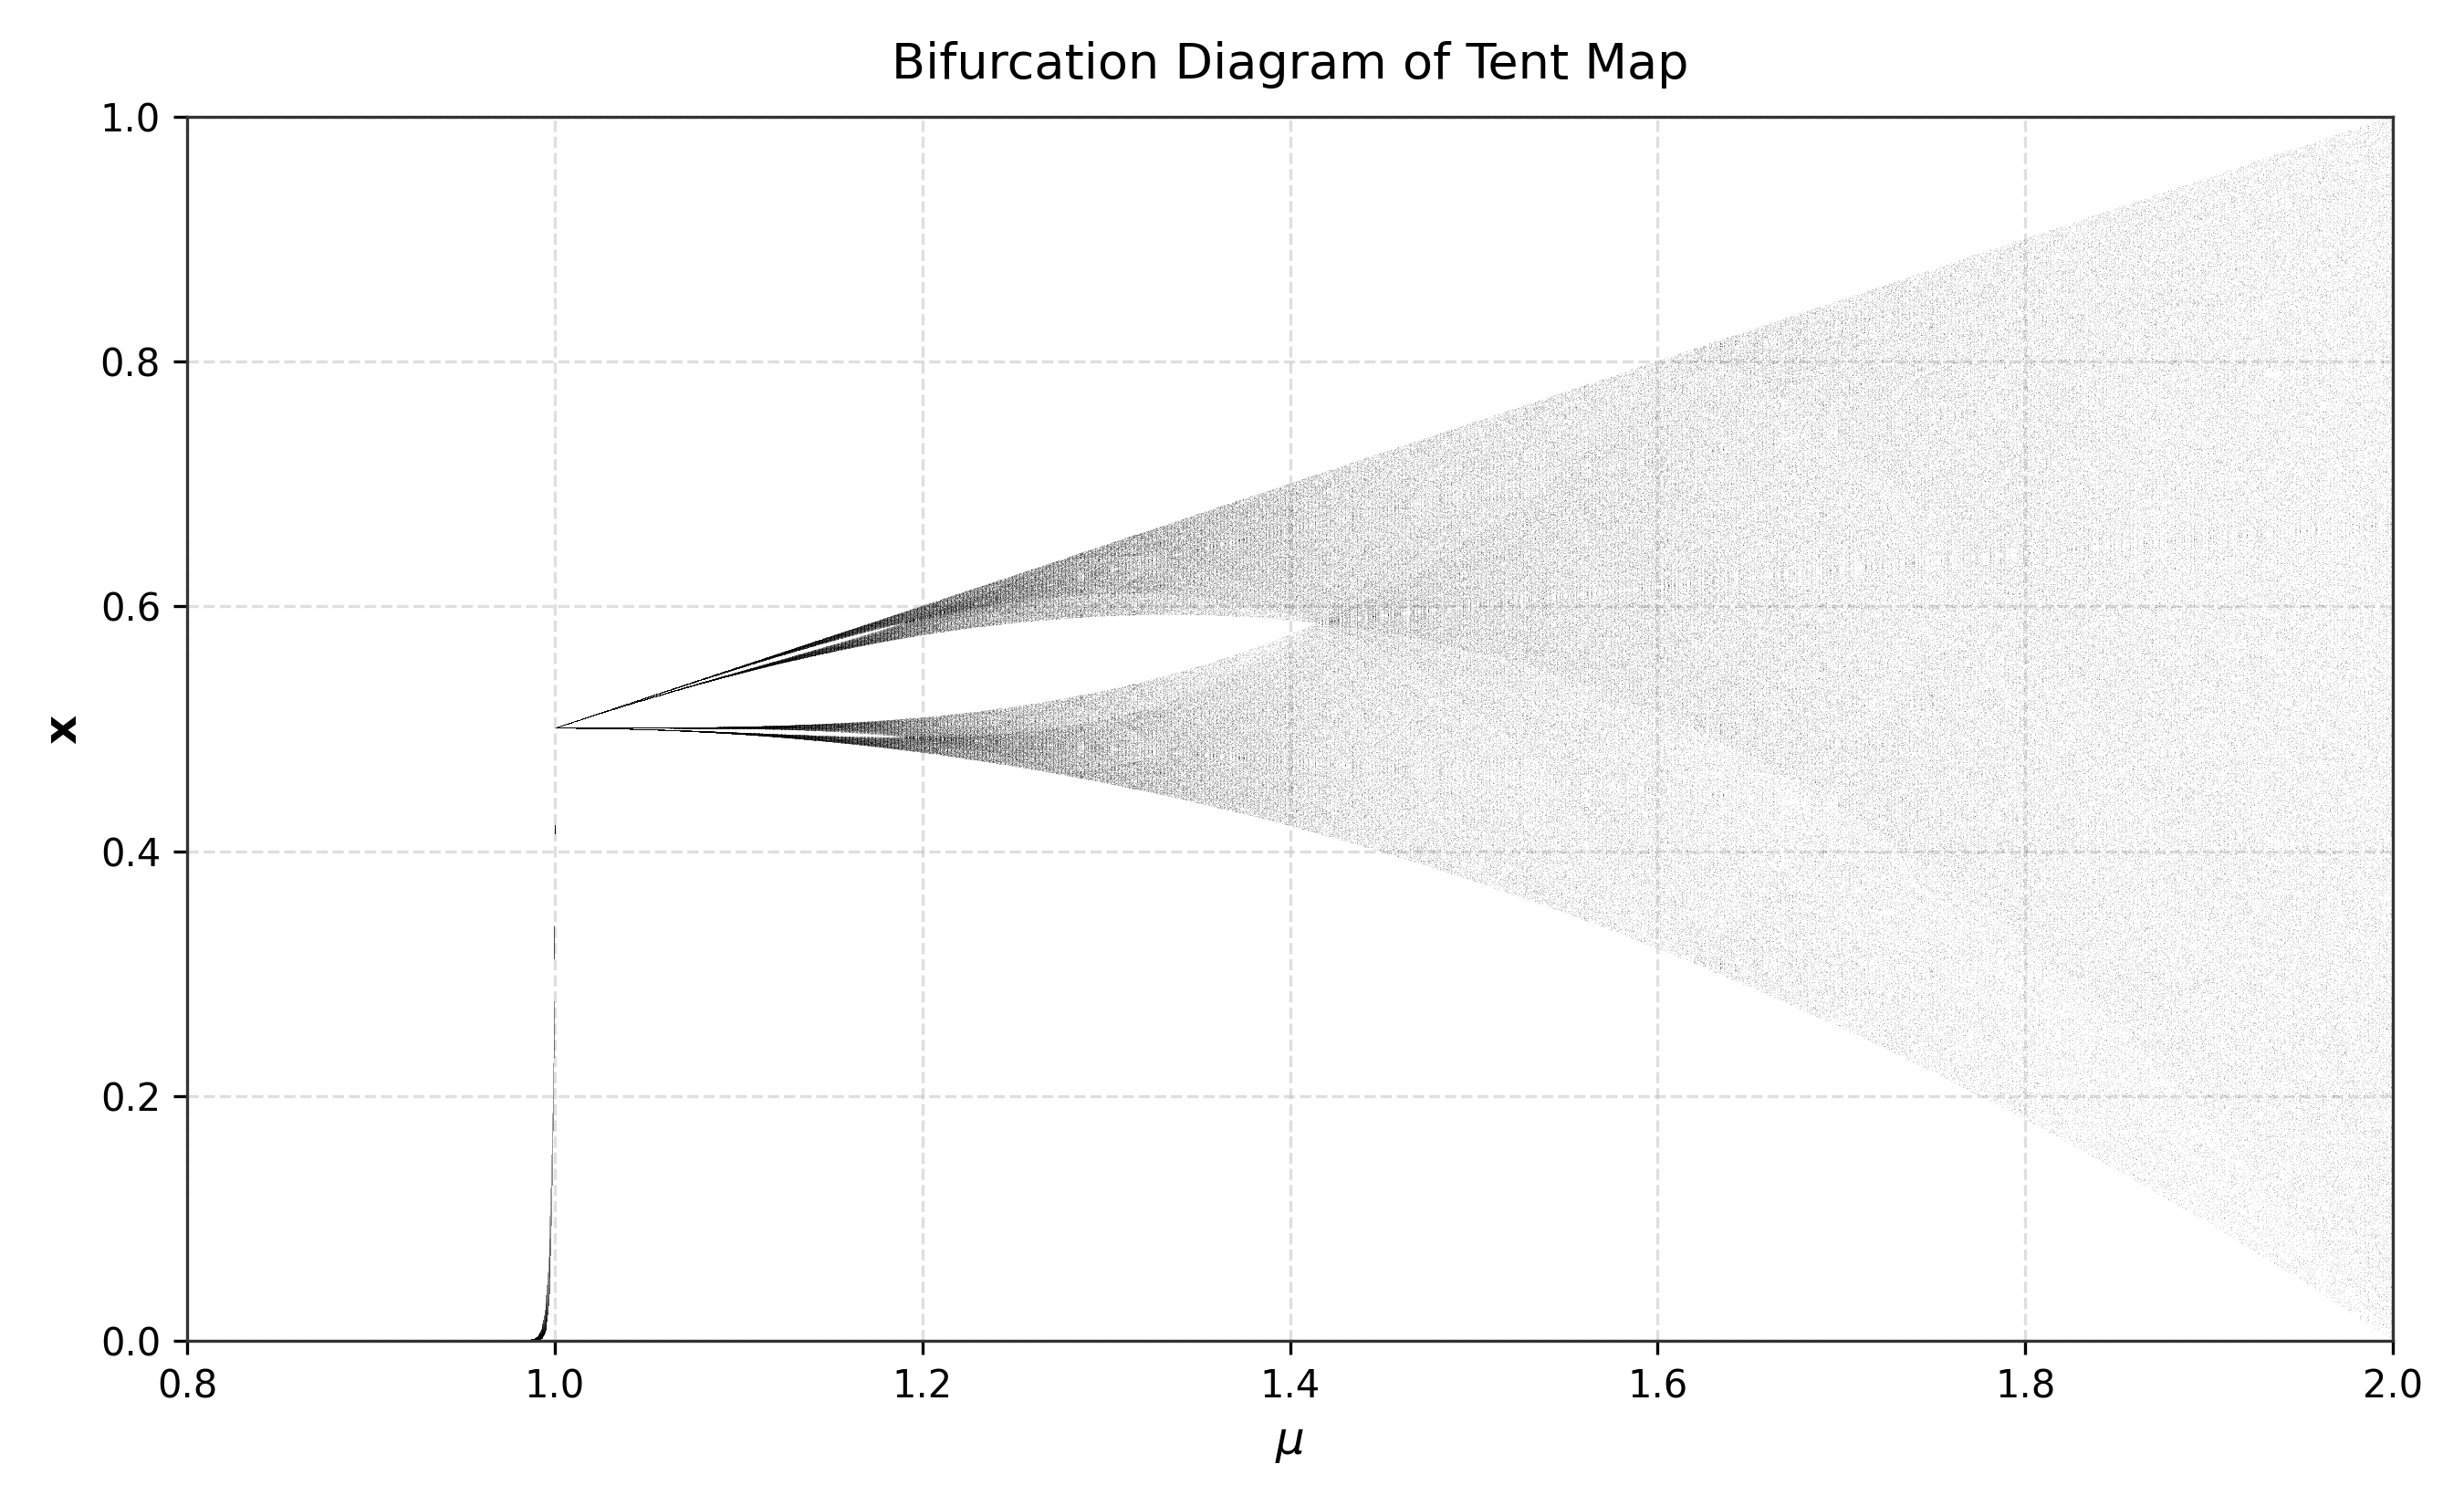
\includegraphics[width=0.75\textwidth]{images/tent_map.png}
    \caption{شکل ‏۲‏-‏۲‏: نمودار انشعاب نگاشت تنت \cite{ref5}}
    
\end{figure}

\subsubsection{‏۲‏-‏۴‏-‏۶‏-‏۴‏ نگاشت سینوسی}

نگاشت سینوسی نسخه‌ای غیرخطی و مثلثاتی از نگاشت‌های آشوبی یک‌بعدی است که به دلیل شکل هموار و پیوسته تابع سینوسی، در ترکیب با سایر نگاشت‌ها برای ساخت سیستم‌های آشوبی نمایی (انتهای این بخش) کاربرد دارد:

\begin{equation}

x_{n+1} = \frac{r}{4}\sin(\pi x_n), \quad r \in (0, 1]
\end{equation}

در رابطه (۲-۳)، $r$ پارامتر دامنه نوسان است. با افزایش $r$ به سمت مقدار بیشینه، رفتار سیستم از حالت تناوبی به آشوبی کامل تغییر می‌کند (شکل ۲-۳). این نگاشت از نظر توپولوژیک با نگاشت لجستیک مرتبط است و می‌تواند رفتار پویای مشابهی از خود نشان دهد\cite{ref5, ref4}.

\begin{figure}[htbp]
    \centering
    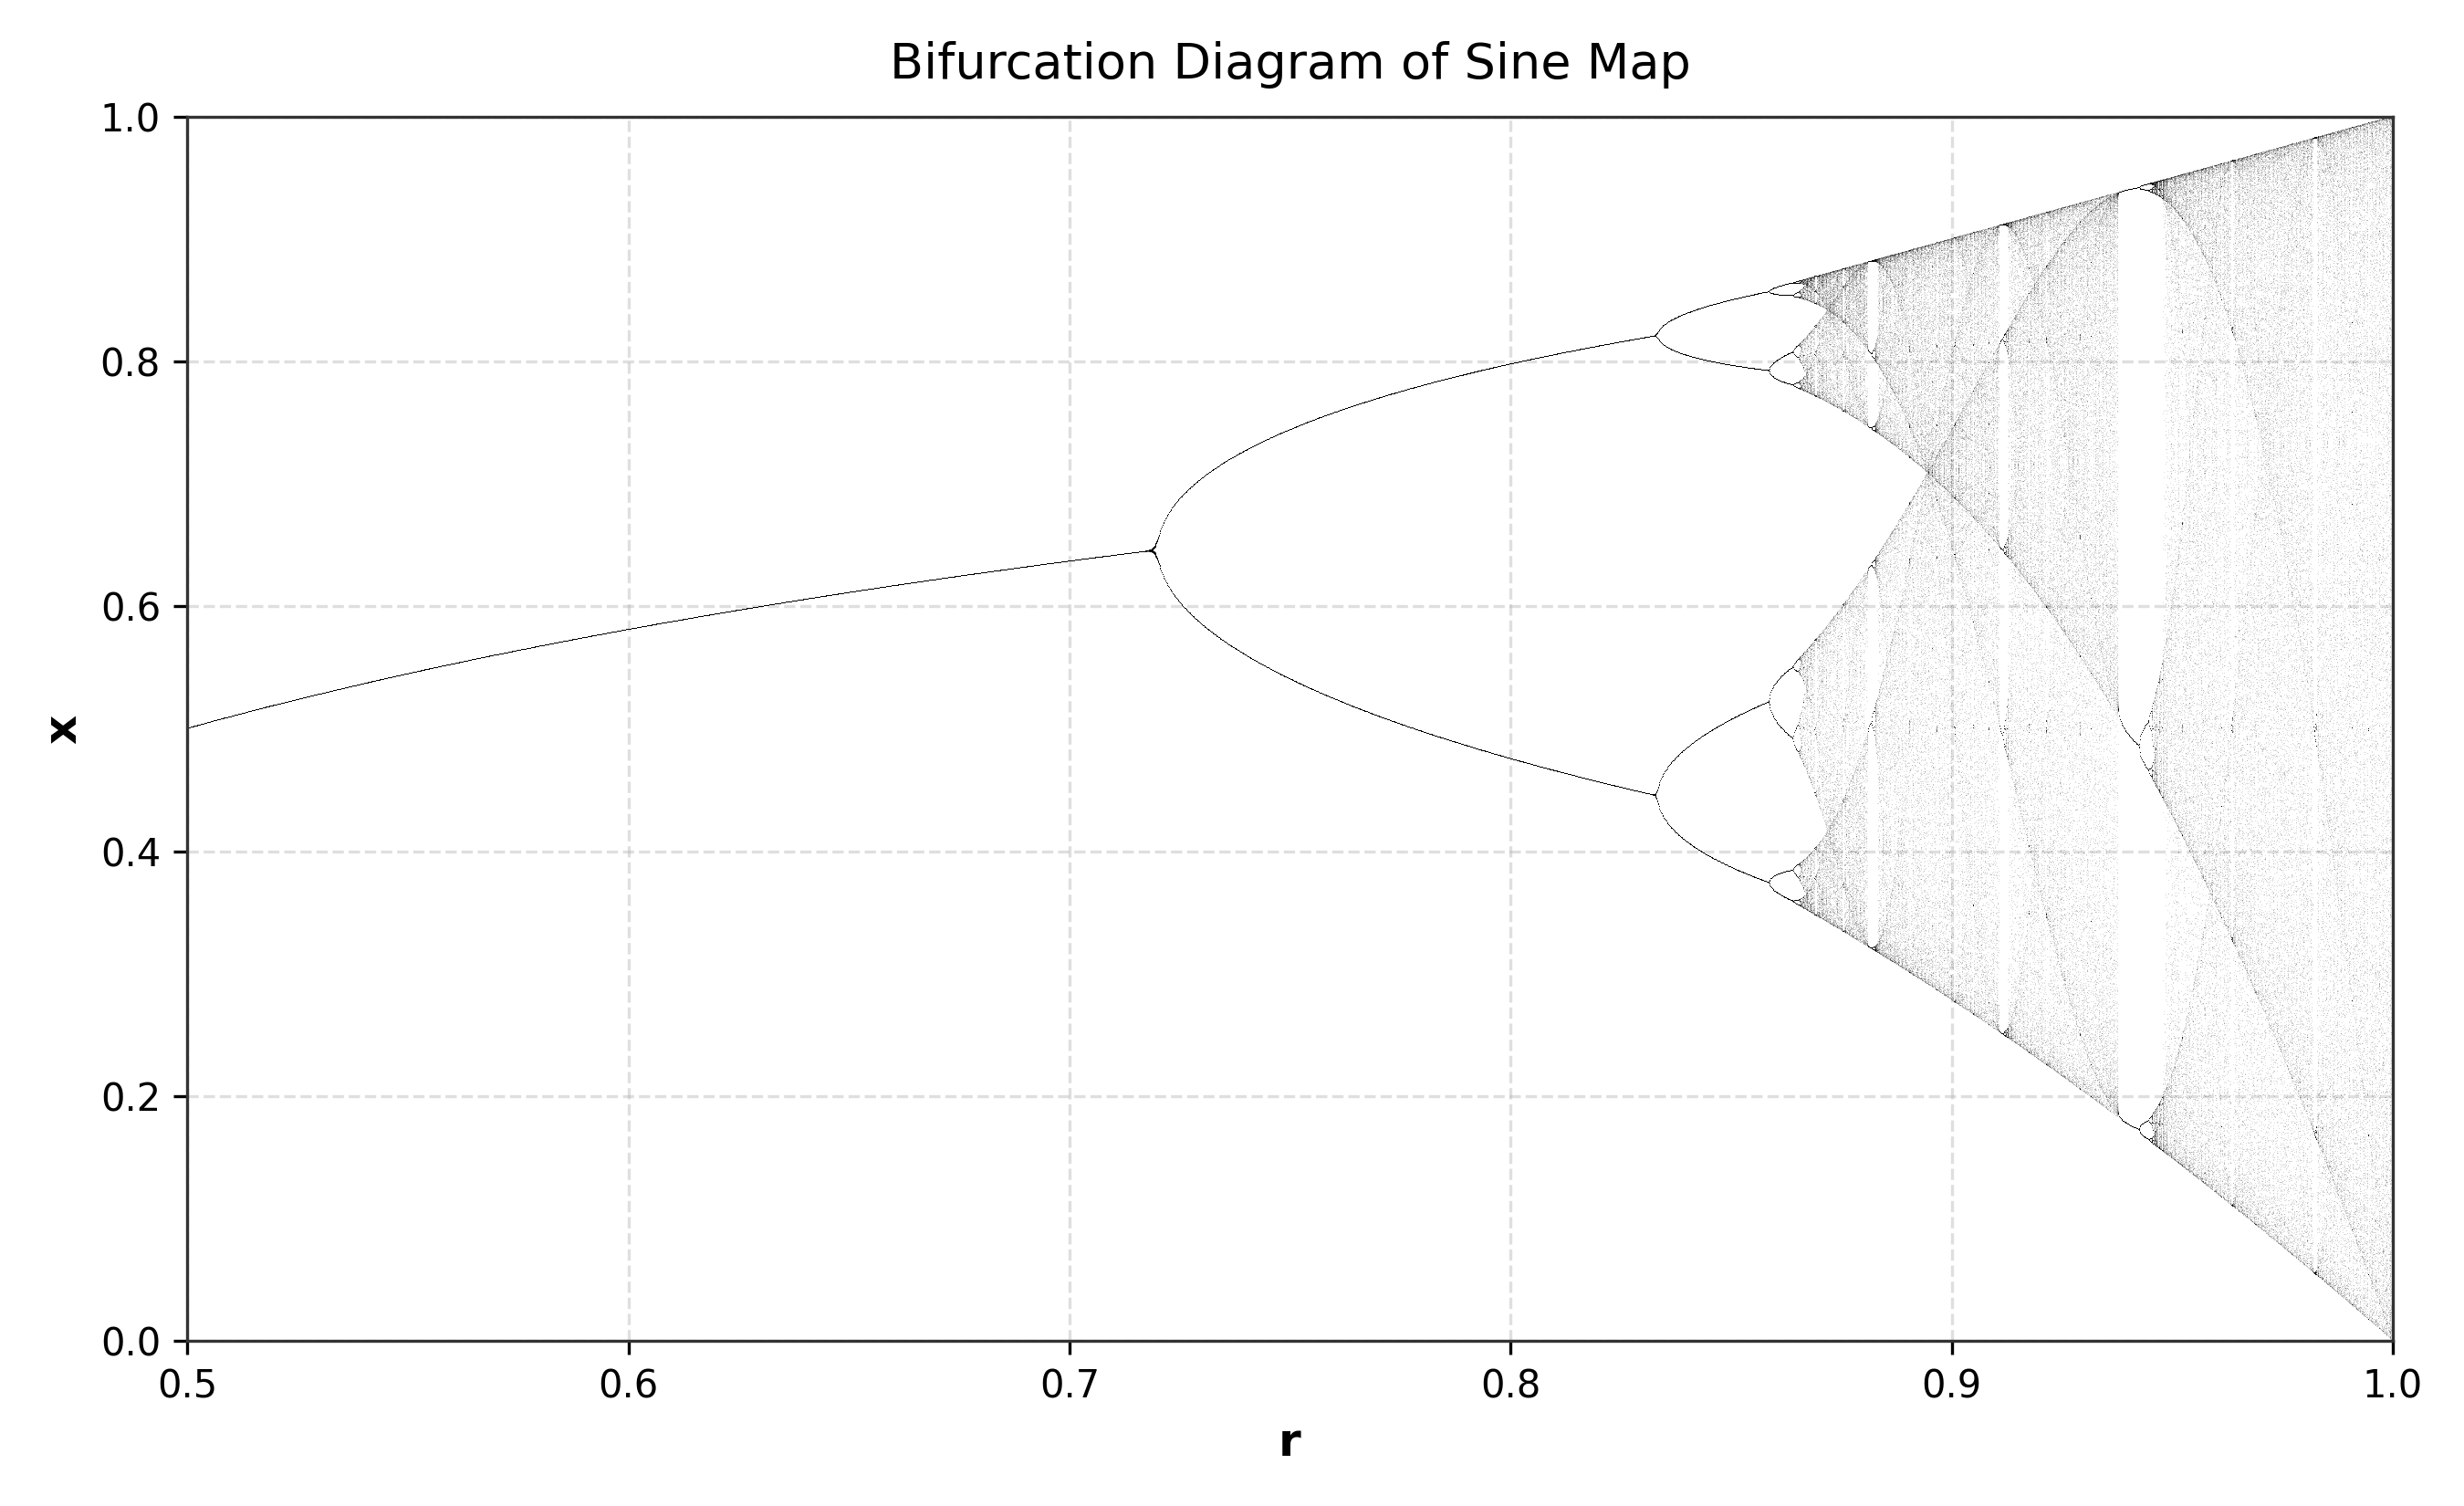
\includegraphics[width=0.75\textwidth]{images/sine_map.png}
    \caption{شکل ‏۲‏-‏۳‏: نمودار انشعاب نگاشت سینوسی \cite{ref5}}
    
\end{figure}

\subsubsection{‏۲‏-‏۴‏-‏۶‏-‏۵‏ نگاشت هنون}

نگاشت هنون یک سیستم آشوبی دوبعدی و گسسته است که در سال 1976 توسط میشل هنون به‌عنوان نسخه ساده‌شده‌ای از سیستم پیوسته لورنز برای مطالعه جاذب‌های عجیب معرفی شد. این نگاشت با دو معادله تفاضلی کوپل‌شده تعریف می‌شود:

\begin{equation}

\begin{cases}
x_{n+1} = 1 - a\, x_n^2 + y_n \\
y_{n+1} = b\, x_n
\end{cases}
\end{equation}

با مقادیر متعارف a=1.4 و b=0.3 در رابطه (۲-۴)، سیستم رفتاری کاملا آشوبی با جاذب عجیب فراکتالی از خود نشان می‌دهد (شکل ۲-۴). ترکیب نگاشت هنون با سایر نگاشت‌های یک‌بعدی مانند تنت، در پژوهش‌های پیشین برای افزایش امنیت الگوریتم‌های رمزنگاری تصویر رنگی به کار رفته است\cite{ref3}.

\begin{figure}[htbp]
    \centering
    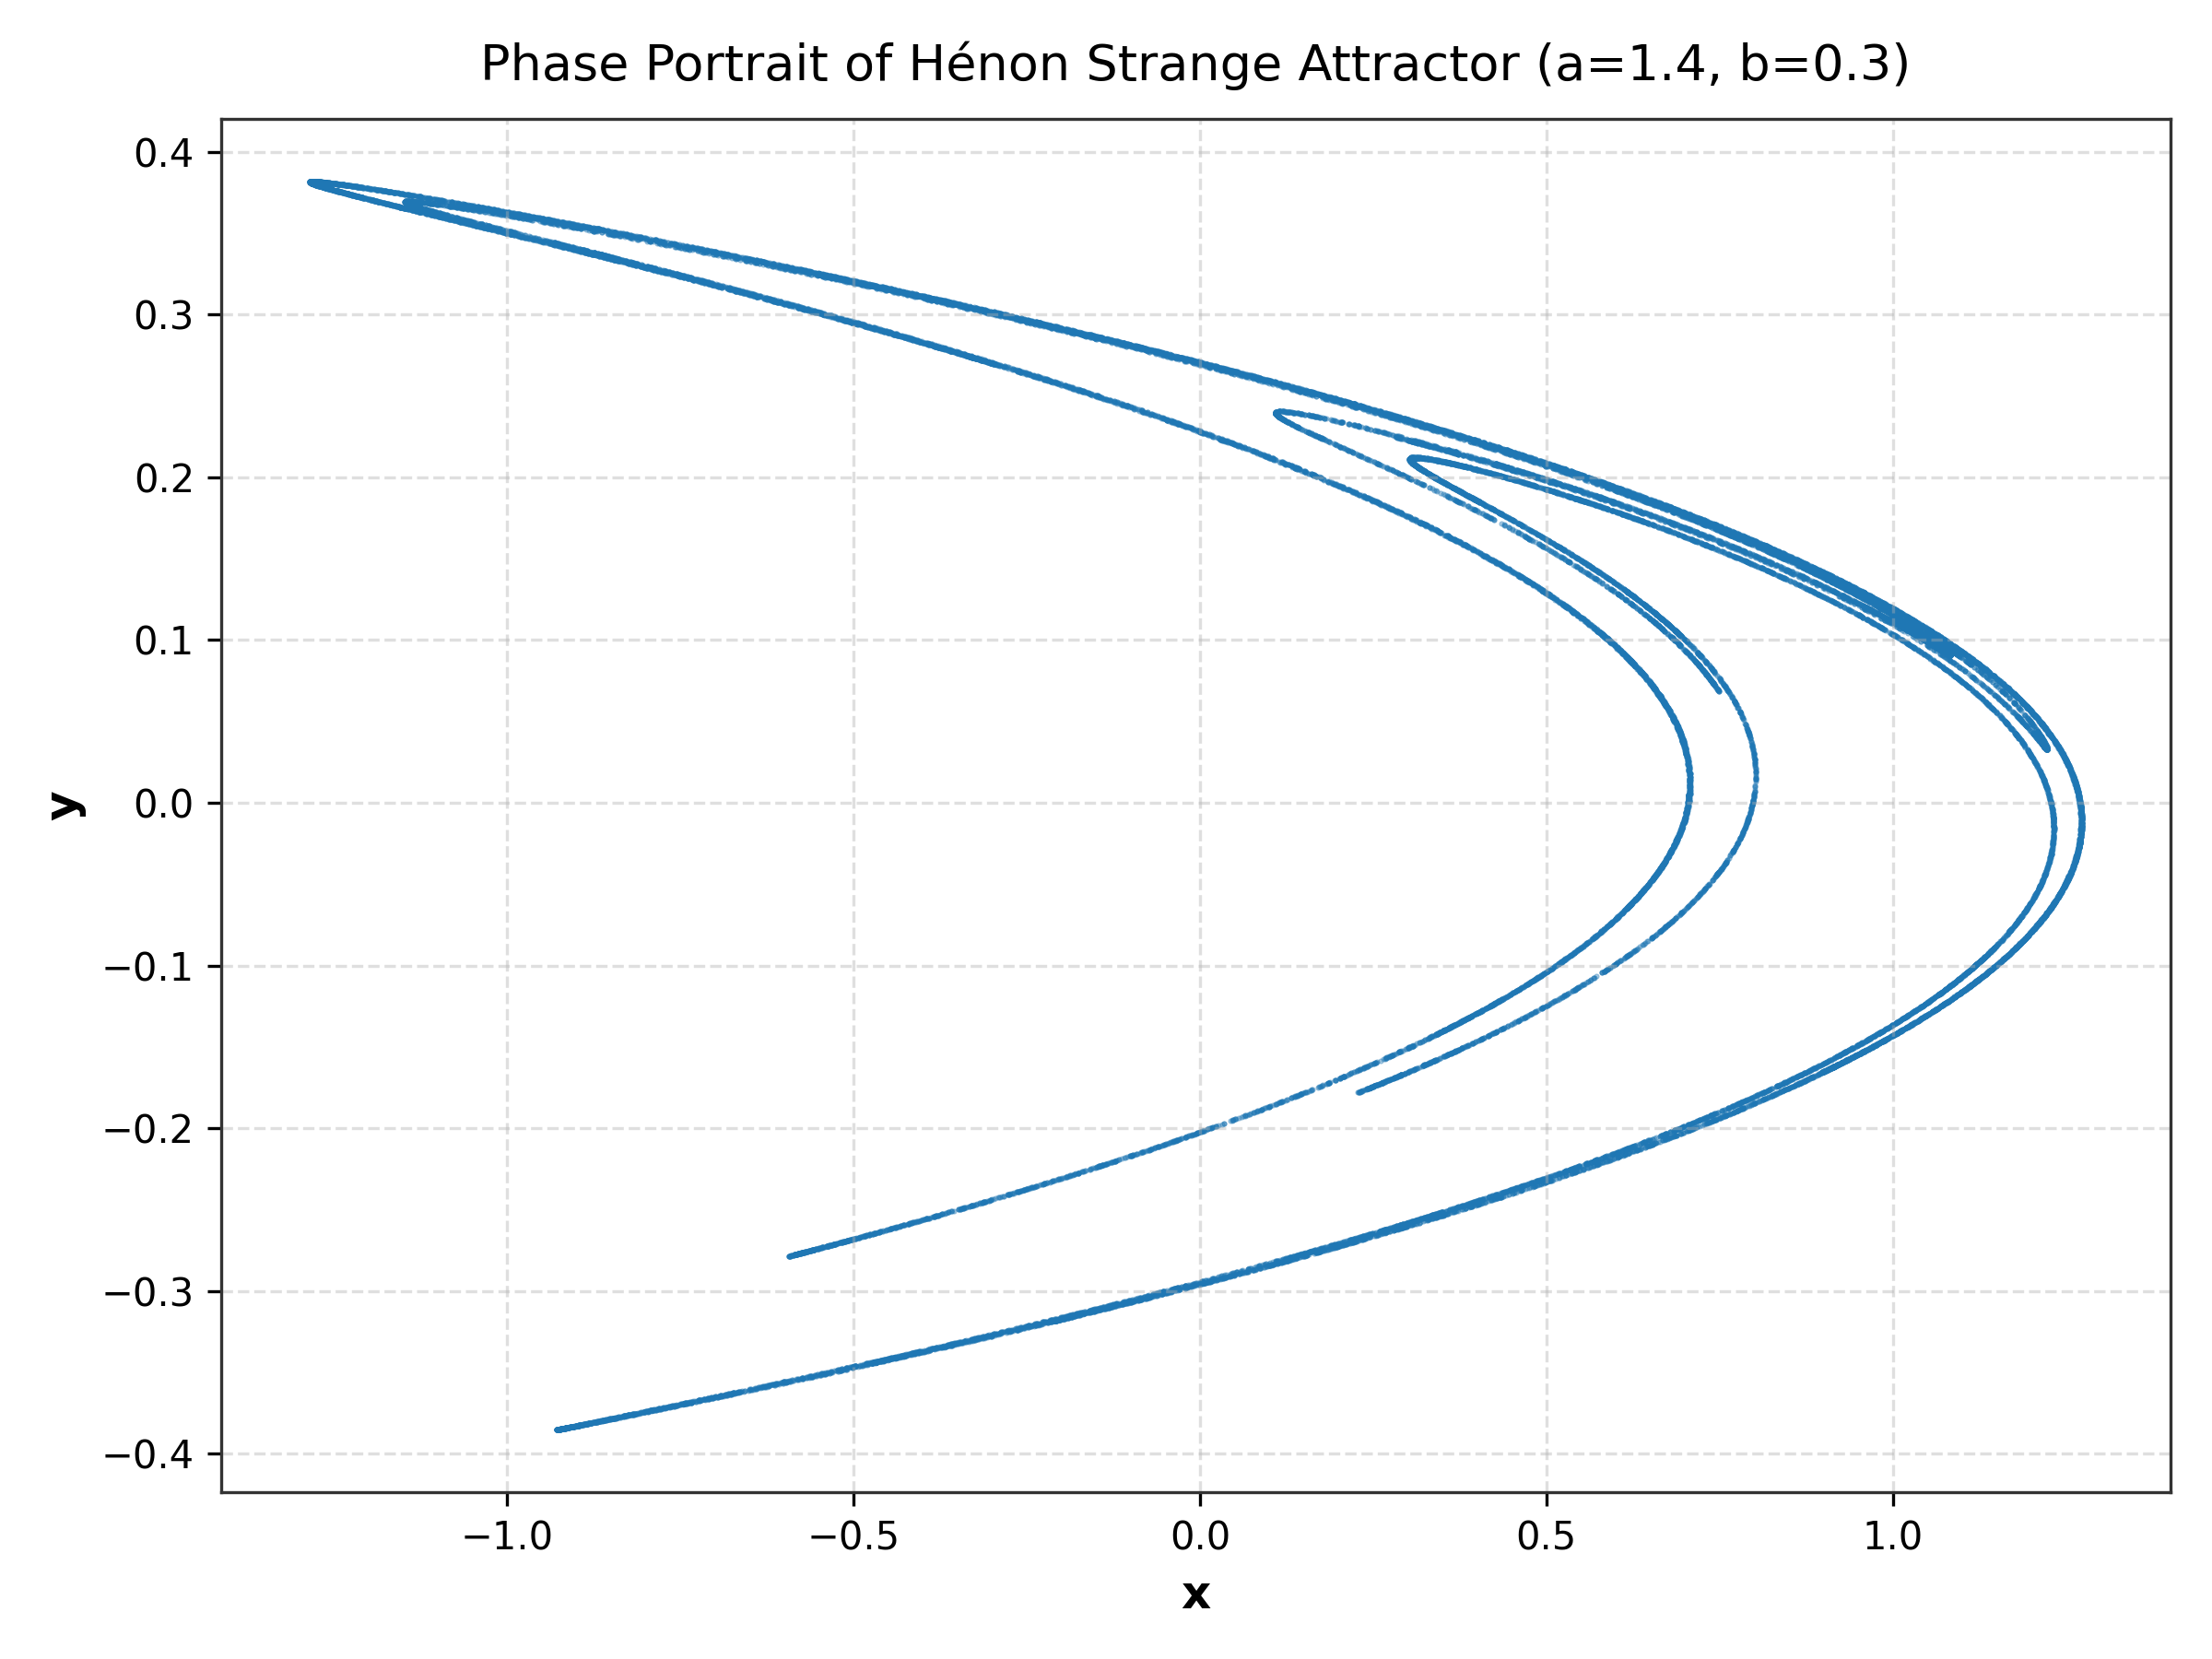
\includegraphics[width=0.75\textwidth]{images/henon_map.png}
    \caption{شکل ‏۲‏-‏۴‏: نمای فضای حالت جاذب آشوبی نگاشت هنون \cite{ref3}}
    
\end{figure}

\subsubsection{‏۲‏-‏۴‏-‏۶‏-‏۶‏ سیستم آشوبی لورنز}

ادوارد لورنز، دانشمند هواشناس، در سال 1963 یک سیستم سه‌معادله‌ای برای مدل‌سازی جابه‌جایی دما به صورت همرفتی در اتمسفر ارائه داد:

\begin{equation}

\left\{ \begin{aligned}
\frac{dx}{dt} &= \sigma (y - x) \\
\frac{dy}{dt} &= x (R - z) - y \\
\frac{dz}{dt} &= xy - \beta z
\end{aligned} \right.
\end{equation}

رابطه (۲-۵) سیستم لورنز است که با مقداردهی به ثابت‌های $\sigma$، R و $\beta$ به عنوان یک سیستم آشوبی، در الگوریتم‌های رمزنگاری کاربرد دارد. این مدل امکان شبیه‌سازی ناپایداری‌ها و پیش‌بینی‌های غیرقطعی در هواشناسی را فراهم می‌کند و به دلیل خواص دینامیکی خاص، گزینه مناسبی برای الگوریتم‌های رمزنگاری محسوب می‌شود (شکل ۲-۵)\cite{ref15, ref16}.

\begin{figure}[htbp]
    \centering
    
\includegraphics[width=0.92\textwidth]{images/image3.png}
    \caption{شکل ‏۲‏-‏۵‏: نمای سه‌بعدی جذب‌کننده آشوبی لورنز \cite{ref23}}
    
\end{figure}

\subsubsection{‏۲‏-‏۴‏-‏۶‏-‏۷‏ سیستم آشوبی چن}

این سیستم در سال 1991 معرفی شد و با معادلات رابطه (۲-۶) نمایش داده می‌شود \cite{ref41}:

\begin{equation}

\begin{cases}
\dot{x} = a (y - x) \\
\dot{y} = (c - a)x - xz + cy \\
\dot{z} = xy - bz
\end{cases}
\end{equation}

با مقادیر اولیه a=35 ، b=3 ، c=28 ، خروجی سیستم به شکل ۲-۶ ترسیم می‌شود. لازم به ذکر است که تغییر هر یک از پارامترهای فوق می‌تواند رفتار سیستم را از حالت آشوبی به غیرآشوبی تغییر دهد. همان‌گونه که در فصل سوم تشریح خواهد شد، این سیستم پیوسته سه‌بعدی در الگوریتم پیشنهادی این پژوهش برای مرحله جایگشت پیکسل‌ها به کار گرفته شده است.

\begin{figure}[htbp]
    \centering
    
\includegraphics[width=0.92\textwidth]{images/image4.png}
    \caption{شکل ‏۲‏-‏۶‏: نمای سه‌بعدی جذب‌کننده آشوبی سیستم چن \cite{ref17}}
    
\end{figure}

\subsubsection{‏۲‏-‏۴‏-‏۶‏-‏۸‏ سیستم‌های آشوبی نمایی}


همان‌گونه که در ابتدای این بخش اشاره شد، نگاشت‌های کلاسیک یک‌بعدی نظیر لجستیک و تنت در پیاده‌سازی دیجیتال با دقت محدود، مستعد پدیده تخریب آشوب هستند. برای رفع این محدودیت، هو و ژو\footnote{Hua and Zhou} \cite{ref4} دسته‌ای از سیستم‌های آشوبی نمایی\footnote{Exponential Chaotic Map (ECM)} را معرفی کردند که مبنای اصلی الگوریتم پیشنهادی این پژوهش را تشکیل می‌دهد. ایده اصلی این رویکرد، ترکیب دو نگاشت آشوبی یک‌بعدی از طریق یک تابع نمایی است تا نگاشت جدیدی با دامنه آشوب پایدار بسیار گسترده‌تر ایجاد شود. ساختار کلی یک نگاشت آشوبی نمایی به‌صورت زیر تعریف می‌شود:

\begin{equation}

f_{\mathrm{ECM}}(x) = f_{\mathrm{outer}}\!\left(\left(e^{\mu \cdot f_{\mathrm{inner}}(x)}\right) \bmod 1\right)
\end{equation}

که در رابطه (۲-۷)، $f_{\mathrm{inner}}$ و $f_{\mathrm{outer}}$ به ترتیب نگاشت‌های آشوبی داخلی و خارجی، و $\mu$ پارامتر نمایی است. با انتخاب هر یک از سه نگاشت پایه لجستیک (روابط ۲-۱)، تنت (رابطه ۲-۲) و سینوسی (رابطه ۲-۳) به‌عنوان $f_{\mathrm{inner}}$ و $f_{\mathrm{outer}}$، در مجموع ۹ نگاشت آشوبی نمایی متمایز حاصل می‌شود که در جدول ۲-۲ فهرست شده‌اند.

\begin{table}[h]
\centering
\small
\begin{tabular}{llll}
\hline
بازه آشوب پایدار & نگاشت خارجی & نگاشت داخلی & نام سیستم \\
$\mu \in (3.57, 4.0)$ & لجستیک & لجستیک & LEL \\
$\mu \in (3.5, 4.0)$ & سینوسی & لجستیک & LES \\
$\mu \in (3.6, 4.0)$ & تنت & لجستیک & LET \\
$\mu \in (0.8\pi, \pi)$ & لجستیک & سینوسی & SEL \\
$\mu \in (0.85\pi, \pi)$ & سینوسی & سینوسی & SES \\
$\mu \in (0.8\pi, \pi)$ & تنت & سینوسی & SET \\
$\mu \in (0.5, 1.0)$ & لجستیک & تنت & TEL \\
$\mu \in (0.5, 1.0)$ & سینوسی & تنت & TES \\
$\mu \in (0.5, 1.0)$ & تنت & تنت & TET \\
\hline
\end{tabular}
\caption{جدول ‏۲‏-‏۲‏: ۹ سیستم آشوبی نمایی حاصل از ترکیب نگاشت‌های پایه \cite{ref4}}

\end{table}

با جایگذاری صریح نگاشت‌های پایه لجستیک ($L$)، تنت ($T$) و سینوسی ($S$) در رابطه (۲-۷)، فرم کامل هر یک از این ۹ سیستم به‌صورت زیر به‌دست می‌آید:

\begin{equation}
x_{n+1} = 4u(1-u), \quad u = \left(e^{\mu\, [4x_n(1-x_n)]}\right) \bmod 1 \qquad (\text{LEL}) 
\end{equation}
\begin{equation}
x_{n+1} = \frac{1}{4}\sin(\pi u), \quad u = \left(e^{\mu\, [4x_n(1-x_n)]}\right) \bmod 1 \qquad (\text{LES}) 
\end{equation}
\begin{equation}
x_{n+1} = T(u), \quad u = \left(e^{\mu\, [4x_n(1-x_n)]}\right) \bmod 1 \qquad (\text{LET}) 
\end{equation}
\begin{equation}
x_{n+1} = 4u(1-u), \quad u = \left(e^{\mu\, [\frac{1}{4}\sin(\pi x_n)]}\right) \bmod 1 \qquad (\text{SEL}) 
\end{equation}
\begin{equation}
x_{n+1} = \frac{1}{4}\sin(\pi u), \quad u = \left(e^{\mu\, [\frac{1}{4}\sin(\pi x_n)]}\right) \bmod 1 \qquad (\text{SES}) 
\end{equation}
\begin{equation}
x_{n+1} = T(u), \quad u = \left(e^{\mu\, [\frac{1}{4}\sin(\pi x_n)]}\right) \bmod 1 \qquad (\text{SET}) 
\end{equation}
\begin{equation}
x_{n+1} = 4u(1-u), \quad u = \left(e^{\mu\, T(x_n)}\right) \bmod 1 \qquad (\text{TEL}) 
\end{equation}
\begin{equation}
x_{n+1} = \frac{1}{4}\sin(\pi u), \quad u = \left(e^{\mu\, T(x_n)}\right) \bmod 1 \qquad (\text{TES}) 
\end{equation}
\begin{equation}
x_{n+1} = T(u), \quad u = \left(e^{\mu\, T(x_n)}\right) \bmod 1 \qquad (\text{TET}) 
\end{equation}

که در آن $T(\cdot)$ همان نگاشت تنت تعریف‌شده در رابطه (۲-۲) است. ویژگی برجسته این ۹ سیستم آن است که خروجی آن‌ها همواره در بازه $[0,1]$ باقی می‌ماند و دامنه آشوب پایدار آن‌ها به‌طور قابل‌توجهی از نگاشت‌های پایه خود گسترده‌تر است\cite{ref4}. این خاصیت امکان انتخاب پویا و تصادفی یکی از این ۹ سیستم برای رمزنگاری هر پیکسل را فراهم می‌سازد، بدون آنکه نگرانی از افت پایداری آشوب طی اجرای طولانی‌مدت الگوریتم وجود داشته باشد. جزئیات کامل پارامترگذاری و نحوه بهره‌گیری از این ۹ سیستم در الگوریتم پیشنهادی، در فصل سوم ارائه شده است.

\section{‏۲‏-‏۵‏ ارتباط بین آشوب و رمزنگاری}

بین سیستم‌های رمزنگاری و سیستم‌های آشوبناک رابطه‌ای بسیار نزدیک وجود دارد و این ارتباط باعث شده است که تئوری آشوب در طراحی رمزنگاری عملی به طور گسترده‌ای مورد استفاده قرار گیرد. نگاشت‌های آشوبناک با رفتار دینامیکی بسیار پیچیده، کاملا قطعی و مشخص هستند و می‌توان آن‌ها را به راحتی با معادلات تفاضلی گسسته مدل‌سازی کرد. به همین دلیل، کارایی رمزنگاری آشوبناک در رمزنگاری تصویر، با توجه به حجم بالای تصاویر، همبستگی پیکسل‌های مجاور و افزونگی موجود در آن، از روش‌های متداول متقارن معمولا بهتر است\cite{ref36}.

خصوصیات دینامیکی نگاشت‌های آشوبناک با ویژگی‌های مورد نیاز یک سیستم رمزنگاری، مانند حساسیت به کلید و متن اصلی، هم‌خوانی زیادی دارد و این مسئله، کاربرد آشوب در رمزنگاری تصاویر را توجیه می‌کند \cite{ref19}. در واقع، اغتشاش\footnote{Ergodicity} در سیستم‌های آشوبناک با اغتشاش\footnote{Confusion} در رمزنگاری متداول، و حساسیت به شرایط اولیه و پارامترهای سیستم آشوبی با انتشار\footnote{Diffusion} و وابستگی به کلید رمز، نظیر یکدیگرند؛ همچنین شرایط اولیه و پارامترهای سیستم آشوبی نقشی مشابه کلید رمز و هر تکرار نگاشت آشوبی نقشی مشابه یک دور\footnote{Cycle} رمزنگاری ایفا می‌کند.

در عمل، اغتشاش در سیستم‌های رمزنگاری متداول از طریق تبدیل متن اصلی به متن تصادفی ایجاد می‌شود، به گونه‌ای که هیچ الگوی تکراری در متن رمز قابل مشاهده نباشد. مشابه این، مسیر حرکت سیستم‌های آشوبناک در فضای حالت معمولا توزیع یکنواخت دارد و پیش‌بینی موقعیت نهایی یک نقطه بر اساس موقعیت اولیه آن بسیار دشوار است\cite{ref23}.

اصل مهم دیگر در طراحی یک سیستم رمزگذاری امن، ویژگی انتشار است. این خاصیت بیان می‌کند که تغییر تنها یک بیت در کلید یا متن اصلی، منجر به تولید یک متن رمز کاملا متفاوت می‌شود. به همین ترتیب، سیستم‌های آشوبناک شدیدا به شرایط اولیه و پارامترهای خود وابسته‌اند و کوچک‌ترین تغییر در نقطه شروع یا پارامترها، باعث انحراف قابل توجه مسیر سیستم می‌شود\cite{ref23}.

تکنیک‌های اصلی رمزنگاری یک بلوک از داده‌ها شامل اغتشاش و انتشار هستند. اغتشاش باعث ایجاد ابهام بین متن اصلی و متن رمز شده می‌شود و انتشار، تغییرات را در سراسر متن رمز پخش می‌کند. جانشینی که در آن یک نماد با نماد دیگری جایگزین می‌شود، ساده‌ترین نوع اغتشاش است. جایگشت که ترتیب عناصر یک بلوک را تغییر می‌دهد، ساده‌ترین روش انتشار محسوب می‌شود.

در سیستم‌های رمزنگاری، جابه‌جایی و جایگزینی متن اصلی به طور مکرر انجام می‌شود تا سطح امنیت مطلوب حاصل شود. هر بار تکرار این عملیات را یک دور می‌نامند. به شکل مشابه، در سیستم‌های دینامیکی، تکرار معادلات تفاضلی در فضای فاز انجام می‌شود. بنابراین، می‌توان از تئوری آشوب برای رمزنگاری بهره برد؛ به گونه‌ای که پارامترها و شرایط اولیه سیستم نقش کلیدی کلید رمز را ایفا کنند و تکرار معادله آشوبناک معادل دورهای عملکرد تابع رمز باشد \cite{ref33}.

\section{‏۲‏-‏۶‏ پیشینه پژوهش}

مطالعات انجام‌شده در زمینه رمزنگاری تصاویر رنگی با استفاده از سیستم‌های آشوبی و الگوریتم‌های بهینه‌سازی در دهه‌های اخیر به‌طور گسترده‌ای مورد توجه قرار گرفته است. در ادامه، به خلاصه‌ای از  تحقیقات داخلی و خارجی مرتبط با موضوع اشاره می‌شود:

ژانگ و لیو\cite{ref3} در مطالعه خود ترکیب سیستم‌های آشوبی نگاشت هنون و نگاشت تنت را برای رمزنگاری تصاویر رنگی پیشنهاد دادند. نتایج این تحقیق نشان داد که این ترکیب، امنیت بیشتری نسبت به استفاده از یک سیستم آشوبی منفرد ارائه می‌دهد و الگوریتم پیشنهادی مقاومت خوبی در برابر حملات آماری دارد.

هو و ژو \cite{ref4} یک مدل آشوبی نمایی برای تولید نگاشت‌های آشوبی یک‌بعدی با آشوب پایدار معرفی می‌کنند. برخلاف بسیاری از سیستم‌های آشوبی که پایداری آشوب را در نظر نمی‌گیرند، این مدل با ترکیب دو سیستم آشوبی یک‌بعدی، نگاشت‌های جدیدی ایجاد می‌کند که در برابر تغییرات پارامتری مقاوم‌اند. در این مقاله، نه سیستم آشوبی مبتنی بر این مدل ارائه شده و رفتار آن‌ها از طریق دیاگرام انشعاب و تحلیل آشوب پایدار بررسی شده است. نتایج ارزیابی عملکرد نشان می‌دهد که این نگاشت‌ها در فضای پارامتری گسترده‌ای آشوب پایدار دارند. همچنین در کاربردهای عملی، این نگاشت‌ها در ارتباطات امن استفاده شده و شبیه‌سازی‌ها، عملکرد برتری را در برابر نویز نشان می‌دهند.

آلوارز و همکاران \cite{ref6} به بررسی رمزنگاری تصاویر با استفاده از سیستم آشوبی لورنز می‌پردازند. با توجه به تبادل گسترده تصاویر حاوی اطلاعات مالی و شخصی در فضای اینترنت، حفاظت از این داده‌ها اهمیت ویژه‌ای دارد. الگوریتم‌های رمزنگاری سنتی عمدتا برای داده‌های متنی طراحی شده‌اند، در حالی که داده‌های چندرسانه‌ای، به‌ویژه تصاویر، کمتر مورد توجه قرار گرفته‌اند. در این پژوهش، روشی برای رمزنگاری و رمزگشایی تصاویر بر پایه سیستم آشوبی لورنز ارائه شده است. در این روش، ابتدا پیکسل‌های تصویر با استفاده از فرآیندهای جابه‌جایی و چرخش معکوس تخریب می‌شوند تا تصادفی‌بودن افزایش یابد. سپس، الگوریتم پیشنهادی با استفاده از معادلات سه‌بعدی سیستم لورنز اجرا می‌شود. نتایج حاصل نشان می‌دهند که میزان آنتروپی تصویر پس از رمزنگاری از 7.285 به 7.9974 افزایش یافته است. همچنین، معیارهای NPCR و UACI به ترتیب 99.65٪ و 30.35٪ محاسبه شده‌اند که نشان‌دهنده قابلیت بالای الگوریتم پیشنهادی در تأمین امنیت اطلاعات تصویری است. مقایسه این روش با سایر تحقیقات مشابه نیز برتری آن را تأیید می‌کند.

خدادادی و زندوکیلی \cite{ref7} روشی نوین برای رمزنگاری تصاویر رنگی با استفاده از ترکیب سیستم‌های آشوبی ارائه داده‌اند که باعث افزایش کارایی و استحکام فرآیند رمزنگاری می‌شود. الگوریتم پیشنهادی سه سری داده در بازه 0 تا 255 را با استفاده از سیستم آشوبی چن تولید می‌کند. سپس، یک سیستم چن دیگر با مقادیر اولیه متفاوت آغاز می‌شود که داده‌ها را به سه سری مقادیر بین 0 تا 10 تبدیل می‌کند. در این روش، مقادیر قرمز، سبز و آبی تصویر با داده‌های تولیدشده از سیستم اول ترکیب شده و برای رمزنگاری اولین پیکسل تصویر استفاده می‌شود. مقادیر تولیدشده از سیستم دوم نیز برای تغییر ترتیب ترکیب مقادیر سیستم اول با پیکسل‌های تصویر به کار گرفته می‌شوند. این فرآیند تا رمزنگاری تمامی پیکسل‌ها ادامه می‌یابد. نوآوری اصلی این روش در استفاده ترکیبی از دو سیستم آشوبی است که پیچیدگی فرآیند رمزنگاری را افزایش می‌دهد. نتایج آزمایش‌ها بر روی تصاویر استاندارد (مجموعه داده‌های USC) کارایی و استحکام این روش را نشان می‌دهد.

پژوهش وانگ و لی \cite{ref8} نشان داد که استفاده از سیستم آشوبی نگاشت لجستیک در ترکیب با جایگشت و انتشار، می‌تواند یک الگوریتم رمزنگاری ایمن برای تصاویر ایجاد کند. با این حال، نیاز به بهبود کارایی محاسباتی الگوریتم برای استفاده در کاربردهای عملی‌تر، همچنان یک چالش باقی می‌ماند. این محدودیت می‌تواند انگیزه‌ای برای پژوهش‌های آینده باشد تا الگوریتم‌های رمزنگاری کارآمدتر و سریع‌تری طراحی شوند.

در پژوهش دیگری از یک سیستم رمزنگاری مبتنی بر آشوب برای رمزگذاری تصاویر رنگی استفاده می‌شود \cite{ref9}. در این روش ابتدا تصویر ورودی به کانال‌های قرمز، سبز و آبی تفکیک شده و هر کانال به‌صورت جداگانه پردازش می‌شود. کلیدهای رمزنگاری با استفاده از نگاشت‌های آشوبی غیرخطی تولید می‌شوند که حساسیت بالایی به شرایط اولیه دارند و کوچکترین تغییر در پارامترهای اولیه، خروجی کاملا متفاوتی ایجاد می‌کند. پیکسل‌های هر کانال ابتدا با دنباله‌های آشوبی جابه‌جا شده و سپس مقادیر آن‌ها با عملیات XOR و جایگزینی دینامیکی تغییر داده می‌شود. در نهایت کانال‌های اصلاح‌شده مجددا ترکیب شده و تصویر رمزگذاری‌شده نهایی حاصل می‌شود. این سیستم با ایجاد توزیع یکنواخت در هیستوگرام و کاهش همبستگی پیکسل‌های مجاور امنیت بالایی در برابر حملات آماری ارائه می‌دهد.

لی و همکاران \cite{ref10} با استفاده از سیستم آشوبی نمائی LEL ، دنباله‌های تصادفی با پیچیدگی بالا تولید کردند. نتایج پژوهش نشان داد که سیستم LEL در مقایسه با سیستم‌های آشوبی رایج، قابلیت بالاتری در تولید توالی‌های غیرقابل پیش‌بینی دارد و امنیت رمزنگاری را افزایش می‌دهد.

صادقیان \cite{ref11} در پژوهشی به بررسی روش جدیدی برای رمزنگاری تصاویر دیجیتال بر اساس ترکیب سیستم‌های آشوبی، الگوریتم ژنتیک و الگوریتم بهینه‌سازی ازدحام ذرات پرداخته است.  با توجه به ویژگی‌های خاص داده‌های تصویری، مانند حجم بالا و همبستگی زیاد میان پیکسل‌های همجوار، استفاده از الگوریتم‌های رمزنگاری متنی ناکارآمد است. در این روش، از سیستم‌های آشوبی برای ایجاد حساسیت به مقادیر اولیه و تولید داده‌های شبه‌تصادفی استفاده شده است. همچنین، ترکیب الگوریتم ژنتیک و PSO به منظور بهینه‌سازی پارامترهای آشوبی و جلوگیری از جستجوی راکد به‌کار گرفته شده است. نتایج به‌دست‌آمده از آزمایش‌های انجام‌شده بر روی مجموعه‌ای از تصاویر استاندارد در نرم‌افزار متلب نشان می‌دهد که روش پیشنهادی در مقایسه با روش‌های مشابه، عملکرد بهتری در حفظ جزئیات تصویری و مقاومت در برابر حملات دارد.

در تحقیق دیگری، یک الگوریتم رمزنگاری تصویر سریع و ایمن مبتنی بر فوق آشوب و عملیات برداری ارائه شده است \cite{ref12}. روش پیشنهادی با کاهش تعداد تکرارهای سیستم فوق آشوب و به‌کارگیری انتخاب‌گر تصادفی، ماتریس کلیدی با تصادفی‌بودن بالا ایجاد می‌کند. همچنین، انتشار مبتنی بر زنجیره‌سازی رمز بلوکی با استفاده از عملیات برداری، رمزنگاری موازی تصویر را بهبود می‌بخشد. نتایج ارزیابی نشان می‌دهند که الگوریتم پیشنهادی تمامی آزمون‌های NIST SP~800-22 را با موفقیت گذرانده، مقدار آنتروپی آن 7.999 بوده و در برابر حملات مختلف ایمن است. همچنین، با میانگین زمان رمزنگاری 0.023 ثانیه، نیازهای انتقال محرمانه تصاویر را برآورده می‌کند.

در سال 2024 یک روش نوین رمزنگاری تصویر رنگی بر پایه ترکیب سه سیستم آشوبی Lorenz، Henon و 2D-Logistic طراحی شده است \cite{ref13}. این الگوریتم به‌صورت مستقل برای هر کانال رنگی عملیات جایگشت و انتشار انجام می‌دهد و با تحلیل‌هایی از جمله آنتروپی شانون، NPCR و UACI نشان داده شد که در برابر حملات آماری و تحلیل کلید مقاومت بالایی دارد.

\subsection{‏۲‏-‏۶‏-‏۱‏ جمع‌بندی پژوهش‌های مرجع}

با توجه به مرور پژوهش‌های فوق، روش‌های رمزنگاری تصویر رنگی مبتنی بر آشوب را می‌توان از منظر سیستم(های) آشوبی به‌کاررفته، سازوکار جایگشت و انتشار، نوآوری الگوریتمی و معیارهای امنیتی گزارش‌شده در کنار هم قرار داد. جدول ۲-۳ خلاصه‌ای تطبیقی از مهم‌ترین مطالعات مرتبط با موضوع پژوهش حاضر ارائه می‌دهد. مقادیر عددی آنتروپی، NPCR و UACI تنها در صورتی درج شده‌اند که در مقاله مرجع گزارش شده باشند؛ در غیر این صورت با «---» مشخص شده است.

همان‌طور که جدول نشان می‌دهد، بیشتر پژوهش‌های پیشین از یک یا دو سیستم آشوبی ثابت (مانند نگاشت لجستیک، نگاشت تنت یا سیستم لورنز) بهره برده‌اند که در سراسر فرآیند رمزنگاری تصویر بدون تغییر باقی می‌ماند. در مقابل، هو و ژو \cite{ref4} با معرفی نه سیستم آشوبی نمایی دارای آشوب پایدار، مجموعه‌ای گسترده‌تر از نگاشت‌های قابل‌استفاده را فراهم کرده‌اند، هرچند این مطالعه به کاربرد این سیستم‌ها در یک الگوریتم کامل رمزنگاری تصویر نپرداخته است.

از نظر معیارهای امنیتی گزارش‌شده، مقادیر آنتروپی در مطالعاتی که این معیار را سنجیده‌اند عموما در بازه‌ی نزدیک به سقف نظری 8 بیت (حدود 7.997 تا 7.999) قرار دارد، بدون آنکه هیچ‌یک به مقدار دقیق و کامل 8.0 برسند؛ این موضوع با ماهیت آماری تصاویر رمزشده سازگار است. به همین ترتیب، مقادیر NPCR گزارش‌شده در پژوهش‌های مرور شده در محدوده‌ی نزدیک به 99.6\% و مقادیر UACI در محدوده‌ی نزدیک به مقدار ایده‌آل نظری 33.46\% قرار می‌گیرند.

با این حال، تنها بخش کوچکی از پژوهش‌های مرور شده (مانند الگوریتم فوق‌آشوب \cite{ref12}) به‌صراحت به زمان اجرا یا هزینه محاسباتی روش پیشنهادی خود اشاره کرده‌اند و اغلب مطالعات دیگر این معیار را گزارش نمی‌کنند. همچنین، ارزیابی روی مجموعه‌ای متنوع از تصاویر استاندارد با ویژگی‌های بافتی متفاوت (مانند تصاویر با جزئیات بالا در مقابل تصاویر یکنواخت) در بسیاری از این مطالعات به‌طور کامل گزارش نشده است. این خلأها، یعنی کمبود گزارش نظام‌مند کارایی محاسباتی و ارزیابی جامع روی تصاویر متنوع در کنار استفاده از سیستم‌های آشوبی متنوع‌تر و انتخاب پویای آن‌ها، انگیزه‌ی اصلی پژوهش حاضر را شکل می‌دهند. مقایسه تفصیلی نتایج روش پیشنهادی با این مطالعات مرجع در فصل پنجم (بحث و نتیجه‌گیری) ارائه خواهد شد.

\begin{table}[h]
\centering
\footnotesize
\resizebox{\textwidth}{!}{%
\begin{tabular}{llllllll}
\hline
مرجع & سیستم(های) آشوبی & جایگشت & انتشار & ویژگی متمایز & آنتروپی & NPCR (\%) & UACI (\%) \\
ژانگ و لیو \cite{ref3} & Henon + Tent & بله & بله & ترکیب دو نگاشت گسسته & --- & --- & --- \\
هو و ژو \cite{ref4} & ۹ ECM & --- & --- & پایداری آشوب نمایی & --- & --- & --- \\
آلوارز \cite{ref6} & Lorenz سه‌بعدی & بله & معادلات لورنز & تمرکز بر تصاویر رنگی & 7.9974 & 99.65 & 30.35 \\
خدادادی \cite{ref7} & Chen + Logistic & بله & ترکیب کانال‌ها & دو سیستم آشوبی متوالی & 7.9971 & 99.58 & 33.21 \\
وانگ و لی \cite{ref8} & Logistic & بله & XOR & سادگی پیاده‌سازی & 7.9968 & 99.57 & 33.38 \\
مقاله \cite{ref9} & نگاشت‌های غیرخطی & بله & XOR دینامیکی & پردازش مستقل کانال‌ها & --- & --- & --- \\
لی \cite{ref10} & LEL نمایی & --- & --- & توالی پرپیچیدگی بالا & --- & --- & --- \\
صادقیان \cite{ref11} & آشوب + GA + PSO & --- & --- & بهینه‌سازی پارامتر & --- & --- & --- \\
فوق‌آشوب \cite{ref12} & Hyper-chaos & بله & زنجیره‌ای & سرعت بالا (0.023\,s) & 7.9990 & 99.61 & 33.46 \\
مقاله \cite{ref13} & Lorenz+Henon+2D-Log & بله & جداگانه per کانال & ترکیب سه سیستم & --- & --- & --- \\
\hline
\end{tabular}%
}
\caption{جدول ‏۲‏-‏۳‏: جمع‌بندی تطبیقی روش‌های رمزنگاری تصویر رنگی مبتنی بر آشوب در پژوهش‌های مرجع}
\end{table}

توضیح: مقادیر آنتروپی، NPCR و UACI مستقیما از گزارش مقالات مرجع استخراج شده‌اند. «---» به معنای عدم گزارش صریح آن معیار در منبع است. ارزیابی و مقایسه دقیق نتایج روش پیشنهادی این پژوهش با این مقادیر در فصل‌های چهارم و پنجم ارائه می‌شود.


@@PB@@


% !TEX root = main.tex
% ============================================================================
% CHAPTER 3: PROPOSED ALGORITHM
% ============================================================================

\chapter{فصل سوم: معرفی الگوریتم پیشنهادی}
\section{‏۳‏-‏۱‏ مقدمه}

این فصل به تشریح دقیق الگوریتم پیشنهادی رمزنگاری تصاویر رنگی اختصاص دارد. هدف اصلی، ارائه توضیح شفاف و کامل از هر یک از مراحل فرآیند رمزنگاری است به‌گونه‌ای که قابل بازتولید و ارزیابی مستقل باشد. نوآوری اصلی این پژوهش در به‌کارگیری ترکیبی پویا و چندلایه از ۹ سیستم آشوبی نمایی در کنار سیستم سه‌بعدی Chen برای جایگشت نهفته است؛ رویکردی که موجب ارتقاء امنیت در برابر انواع حملات تحلیل آماری، دیفرانسیلی و جستجوی فراگیر می‌شود.

ساختار این فصل بر سه محور اصلی استوار است: نخست، تعریف و توجیه انتخاب مؤلفه‌های الگوریتم؛ دوم، تشریح گام‌به‌گام فرآیند رمزنگاری و رمزگشایی با ارائه روابط ریاضی دقیق؛ و سوم، معرفی روش پیاده‌سازی و ابزارهای ارزیابی که در فصل چهارم مورد استفاده قرار خواهند گرفت.

\section{‏۳‏-‏۲‏ معرفی سیستم‌های آشوبی مورد استفاده}

\subsection{‏۳‏-‏۲‏-‏۱‏ سیستم آشوبی سه‌بعدی Chen}

سیستم آشوبی Chen  \cite{ref6} یک سیستم دینامیکی پیوسته سه‌بعدی از خانواده سیستم‌های ابرجاذبی است که در سال 1999 معرفی شد. این سیستم از سه معادله دیفرانسیل غیرخطی کوپل‌شده تشکیل شده و جاذب آشوبی آن طیف لیاپانوف مثبت گسترده‌ای دارد. ویژگی‌هایی نظیر حساسیت فوق‌العاده بالا به شرایط اولیه، پویایی سه‌بعدی پیچیده و تولید دنباله‌های شبه‌تصادفی با توزیع گسترده، این سیستم را به گزینه‌ای ایده‌آل برای مرحله جایگشت تبدیل کرده‌اند.

معادلات حاکم بر سیستم Chen به‌صورت زیر تعریف می‌شوند:

\begin{equation}

\begin{cases}
\dot{x} = a(y-x) \\
\dot{y} = (c-a)x - xz + cy \\
\dot{z} = xy - bz
\end{cases}
\end{equation}

در این معادلات، $x(t)$، $y(t)$ و $z(t)$ متغیرهای حالت سیستم در زمان $t$ هستند. پارامترهای $a$، $b$ و $c$ ثابت‌های سیستمی هستند که رفتار آشوبی را تعریف می‌کنند. مقادیر استاندارد اثبات‌شده برای ایجاد آشوب پایدار در این سیستم عبارتند از: a=35, b=3, c=28

این مقادیر در مقاله \cite{ref6} توسط Chen و Ueta تأیید شده‌اند و در بازه وسیعی از مطالعات رمزنگاری آشوبی به‌کار رفته‌اند. با این پارامترها، نمای لیاپانوف سیستم مثبت است ($\lambda_1 \approx 2.03$) که وجود آشوب را تضمین می‌کند. شرایط اولیه سیستم Chen یعنی مقادیر $x_0$، $y_0$ و $z_0$ بخش اصلی کلید رمزنگاری را تشکیل می‌دهند و باید به‌صورت دقیق با دقت اعشاری $10^{-15}$ حفظ شوند. هرگونه انحراف جزئی از این مقادیر، دنباله جایگشتی کاملاً متفاوتی تولید می‌کند و رمزگشایی را ناممکن می‌سازد.

\subsection{‏۳‏-‏۲‏-‏۲‏ نگاشت‌های آشوبی نمایی (ECM)}

سیستم‌های آشوبی نمایی توسط هو و ژو \cite{ref4}معرفی شده‌اند. ایده اصلی این رویکرد، ترکیب دو نگاشت آشوبی یک‌بعدی از طریق یک تابع نمایی است تا نگاشت جدیدی با پایداری آشوب بسیار بالاتر ایجاد شود. این رویکرد به‌طور مؤثری پدیده تخریب آشوب را که در نگاشت‌های کلاسیک مانند Logistic و Tent مشاهده می‌شود، برطرف می‌کند.

ساختار کلی یک نگاشت آشوبی نمایی به‌صورت زیر تعریف می‌شود:

\begin{equation}

f_{\mathrm{ECM}}(x) = f_{\mathrm{outer}}\!\left(\exp(\mu \cdot f_{\mathrm{inner}}(x))\right) \bmod 1
\end{equation}

در این رابطه، $f_{\mathrm{inner}}$ نگاشت آشوبی داخلی، $f_{\mathrm{outer}}$ نگاشت آشوبی خارجی، $\mu$ پارامتر نمایی و $x$ متغیر حالت است. ترکیب سه عنصر Logistic (L)، Sine (S) و Tent (T) در نقش داخلی و خارجی، ۹ نگاشت متمایز ایجاد می‌کند:

\begin{table}[h]
\centering
\small
\begin{tabular}{llll}
\hline
بازه آشوب پایدار & نگاشت خارجی & نگاشت داخلی & نام سیستم \\
$\mu \in (3.57, 4.0)$ & Logistic & Logistic & LEL \\
$\mu \in (3.5, 4.0)$ & Sine & Logistic & LES \\
$\mu \in (3.6, 4.0)$ & Tent & Logistic & LET \\
$\mu \in (0.8\pi, \pi)$ & Logistic & Sine & SEL \\
$\mu \in (0.85\pi, \pi)$ & Sine & Sine & SES \\
$\mu \in (0.8\pi, \pi)$ & Tent & Sine & SET \\
$\mu \in (0.5, 1.0)$ & Logistic & Tent & TEL \\
$\mu \in (0.5, 1.0)$ & Sine & Tent & TES \\
$\mu \in (0.5, 1.0)$ & Tent & Tent & TET \\
\hline
\end{tabular}
\caption{جدول ‏۳‏-‏۱‏: ۹ سیستم آشوبی نمایی مورد استفاده در الگوریتم پیشنهادی}
\end{table}

ویژگی برجسته این ۹ سیستم آن است که هریک از آن‌ها دامنه آشوب پایدار گسترده‌ای دارند و خروجی آن‌ها در بازه $[0,1]$ قرار می‌گیرد\cite{ref4, ref1}. این خاصیت انتخاب تصادفی سیستم رمزکننده برای هر پیکسل را ممکن می‌سازد بدون آنکه نیاز به بررسی پایداری در هر مرحله باشد.

روابط دقیق هر یک از نگاشت‌های اصلی تشکیل‌دهنده ECM به‌صورت زیر تعریف می‌شوند:

\begin{itemize}
    \item نگاشت لجستیک:
    \begin{equation}
    L(x) = r\,x\,(1-x), \quad r=4
    
    \end{equation}
    که در آن $r=4$ برای حالت آشوب کامل در نظر گرفته می‌شود.
\end{itemize}

\begin{itemize}
    \item نگاشت سینوسی:
    \begin{equation}
    S(x) = \frac{r}{4}\sin(\pi x), \quad r \in (0,1]
    
    \end{equation}
\end{itemize}

\begin{itemize}
    \item نگاشت تنت:
    \begin{equation}
    T(x) = \begin{cases}
    2x, & x < 0.5 \\
    2(1-x), & x \geq 0.5
    \end{cases}
    
    \end{equation}
\end{itemize}

\section{‏۳‏-‏۳‏ اثبات ریاضی و تحلیل فضای کلید}

امنیت هر الگوریتم رمزنگاری در برابر حملات جستجوی فراگیر\footnote{Brute-Force Attack} به‌طور مستقیم به اندازه فضای کلید\footnote{Key Space} وابسته است. بر اساس استانداردهای بین‌المللی مانند NIST، فضای کلید یک سامانه رمزنگاری\footnote{Cryptosystem} امن باید حداقل بزرگتر از $2^{128}$ باشد تا با قدرتمندترین سوپرکامپیوترهای فعلی و آتی نیز غیرقابل شکست باشد. در الگوریتم پیشنهادی، کلید رمزنگاری از مجموعه‌ای از پارامترهای پیوسته و گسسته تشکیل شده است.

جدول ۳-۲ سهم هر یک از پارامترها و دامنه تغییرات آن‌ها را نشان می‌دهد:

\begin{table}[h]
\centering
\small
\begin{tabular}{lllll}
\hline
فضای حالات موثر & دقت اعشار & بازه کلید & نوع & مؤلفه کلید \\
$10^{15}$ & $10^{-15}$ & (0, 1) & پیوسته & $x_0$ (شرط اولیه Chen) \\
$10^{15}$ & $10^{-15}$ & (0, 1) & پیوسته & $y_0$ (شرط اولیه Chen) \\
$10^{15}$ & $10^{-15}$ & (0, 30) & پیوسته & $z_0$ (شرط اولیه Chen) \\
$10^{15}$ & $10^{-15}$ & (0, 1) & پیوسته & $x_{\mathrm{sel},0}$ (شرط اولیه سلکتور) \\
$10^{15}$ & $10^{-15}$ & (0, 1) & پیوسته & $x_{\mathrm{ecm},0}$ (شرط اولیه ECM) \\
$10^{15}$ & $10^{-15}$ & (3.5, 4.0) & پیوسته & $\mu$ (پارامتر نمایی ECM) \\
$10^{15}$ & $10^{-15}$ & (0, 1) & پیوسته & $x_{\mathrm{final},0}$ (شرط اولیه مرحله ۵) \\
\hline
\end{tabular}
\caption{جدول ‏۳‏-‏۲‏: مؤلفه‌های فضای کلید و اثبات ریاضی سهم هر پارامتر}
\end{table}

\subsection{‏۳‏-‏۳‏-‏۱‏ استخراج دقیق ریاضی فضای کلید}

در محاسبات شناور با دقت مضاعف (Double-Precision Floating-Point مطابق استاندارد IEEE 754)، حساسیت سیستم‌های آشوبی پیشنهادی به شرایط اولیه در حدود $10^{-15}$ است. بنابراین، تعداد حالات مستقل برای هر یک از هفت پارامتر برابر با $N_i = 10^{15}$ است.

مجموع کل حالت‌های کلید از ضرب فضای حالت تمام پارامترهای مستقل به دست می‌آید:

\begin{equation}
|K| = \Delta x_0 \times \Delta y_0 \times \Delta z_0 \times \Delta x_{\mathrm{sel}} \times \Delta x_{\mathrm{ecm}} \times \Delta \mu \times \Delta x_{\mathrm{final}}

\end{equation}

با جایگذاری مقادیر در رابطه فوق:

\begin{equation}
|K| = 10^{15} \times 10^{15} \times 10^{15} \times 10^{15} \times 10^{15} \times 10^{15} \times 10^{15} = 10^{105}

\end{equation}

برای تبدیل این مقدار به مبنای ۲ (جهت مقایسه با استانداردهای رمزنگاری مانند AES):

\begin{equation}
|K| = 10^{105} = (2^{\log_2 10})^{105} \approx (2^{3.321928})^{105} = 2^{348.8} \approx 2^{350}

\end{equation}

همچنین اگر انتخاب پویا از میان ۹ نگاشت نمایی در لایه انتشار نیز به عنوان یک متغیر ساختاری در نظر گرفته شود، تعداد ترکیب‌های ممکن برای یک تصویر $H \times W$ برابر $9^{H \times W}$ خواهد بود که فضای کلید موثر عملیاتی را به مراتب فراتر از $2^{350}$ افزایش می‌دهد. 

چون $2^{350} \gg 2^{128}$، اثبات می‌شود که الگوریتم پیشنهادی کاملاً در برابر تمامی حملات جستجوی فراگیر و کدهای موازات‌یافته بر روی سیستم‌های ابررایانه‌ای ایمن می‌باشد.

\subsection{‏۳‏-‏۳‏-‏۲‏ توجیه علمی ساختار کلید و عدم استفاده از پارامترهای ثابت به عنوان کلید}
یک سوال کلیدی در تحلیل امنیت الگوریتم‌های مبتنی بر آشوب، دلیل عدم گنجاندن پارامترهای ثابت سیستم‌های آشوبی (مانند پارامترهای سیستم چن $a=35, b=3, c=28$ و پارامتر کنترل نگاشت‌های نمایی $\mu$) در کلید رمزنگاری است. این تصمیم طراحی مبتنی بر دلایل علمی و امنیتی زیر است:
\begin{itemize}
    \item \textbf{تضمین رفتار آشوبی سیستم (محدوده جاذب آشوب):} سیستم‌های آشوبی تنها در بازه‌های مشخصی از پارامترهای خود رفتار آشوب‌گونه نشان می‌دهند. برای مثال، سیستم چن در مقادیر $a=35, b=3, c=28$ دارای جاذب آشوبی پایدار است و نگاشت‌های نمایی نیز برای $\mu \in [3.5, 4.0]$ رفتار آشوب کامل دارند. اگر این پارامترها به عنوان بخشی از کلید رمزنگاری در اختیار کاربر قرار گیرند، تضمینی برای انتخاب مقادیر مناسب وجود ندارد. ورود مقادیری خارج از این محدوده‌ها توسط کاربر می‌تواند سیستم را به سمت مدارهای دوره‌ای ساده یا نقاط همگرا سوق دهد که این امر به تخریب کامل امنیت الگوریتم منجر می‌شود. بنابراین، ثابت نگه‌داشتن این پارامترها و خارج کردن آن‌ها از کلید، یک ضرورت امنیتی برای تضمین رفتار آشوبگون سیستم است.
    \item \textbf{انطباق با اصل کرکوفس (Kerckhoffs's Principle):} بر اساس این اصل بنیادی در رمزنگاری، امنیت یک سیستم باید تنها به محرمانه بودن کلید وابسته باشد و فاش شدن جزئیات الگوریتم (شامل پارامترهای ثابت سیستم‌های آشوبی) نباید خللی در امنیت آن ایجاد کند. در الگوریتم پیشنهادی، امنیت به‌طور کامل توسط شرایط اولیه ($x_0, y_0, z_0, x_{\mathrm{sel},0}, x_{\mathrm{ecm},0}, x_{\mathrm{final},0}$) تامین می‌شود که مستقل از پارامترهای ثابت سیستم هستند.
    \item \textbf{کفایت امنیتی فضای کلید فعلی:} فضای کلید به دست آمده برابر با $2^{350}$ است که بسیار بزرگتر از حداقل آستانه امنیتی مورد نیاز ($2^{128}$) و حتی استاندارد صنعتی رمزنگاری متقارن ($2^{256}$ در AES-256) می‌باشد. افزایش بیهوده پارامترهای کلید (مثلاً اختصاص شرایط اولیه و پارامترهای مستقل به هر یک از نه نگاشت آشوبی) هیچ مزیت امنیتی عملی ایجاد نکرده، اما بار محاسباتی و پیچیدگی مدیریت و انتقال کلید (Key Management) را به شدت افزایش می‌دهد.
    \item \textbf{امنیت ساختاری در مقابل تنوع پارامتری:} نوآوری اصلی این الگوریتم، انتخاب پویای نگاشت آشوبی برای هر پیکسل بر اساس دنباله انتخاب‌گر است. این ویژگی ساختاری تضمین می‌کند که حتی در صورت یکسان بودن شرایط اولیه اولیه نگاشت‌های نمایی، به دلیل تغییر مکرر و شبه‌تصادفی نوع نگاشت در طول پیکسل‌ها، مهاجم قادر به بازسازی دینامیک سیستم نخواهد بود.
\end{itemize}

\section{‏۳‏-‏۴‏ الگوریتم پیشنهادی: توضیح گام‌به‌گام}

الگوریتم رمزنگاری پیشنهادی از پنج مرحله اصلی تشکیل شده است. در ادامه، هر مرحله با جزئیات کامل ریاضی تشریح می‌شود.

\subsubsection{‏۳‏-‏۴‏-‏۱‏ مرحله ۱: تولید کلیدهای اولیه و آماده‌سازی}

در این مرحله، تمام پارامترهای مورد نیاز الگوریتم تولید و مقداردهی اولیه می‌شوند. کلید رمزنگاری $K$ شامل هفت عدد مثبت پیوسته با دقت ۱۵ رقم اعشار است:

تصویر رنگی ورودی با ابعاد $H \times W \times 3$ بارگذاری شده و کانال‌های R، G و B آن تفکیک می‌شوند. هر کانال به‌صورت مستقل پردازش می‌شود. مجموع تعداد پیکسل‌های هر کانال $N = H \times W$ است.

به‌منظور حذف ترانزیت اولیه سیستم آشوبی و اطمینان از رسیدن به ناحیه آشوبی پایدار، سیستم Chen برای ۱۰۰۰ گام اولیه اجرا شده و این مقادیر دور انداخته می‌شوند.  این کار یک الزام علمی برای جلوگیری از ارتباط احتمالی بین کلید و خروجی اولیه است.

\subsubsection{‏۳‏-‏۴‏-‏۲‏ مرحله ۲: جایگشت پیکسل‌ها با سیستم Chen}

هدف این مرحله، از بین بردن همبستگی مکانی بین پیکسل‌های مجاور از طریق جابه‌جایی تصادفی موقعیت آن‌هاست. سیستم Chen با شرایط اولیه ($x_0$, $y_0$, $z_0$) و پارامترهای a=35, b=3, c=28 حل می‌شود.

معادلات دیفرانسیل سیستم Chen با استفاده از حل‌کننده عددی RK45 (روش رانگ-کوتای مرتبه ۴ و ۵) با گام زمانی dt=0.002 حل می‌شوند.  برای هر تصویر با N پیکسل، N + 1000 نقطه زمانی تولید می‌شود که ۱۰۰۰ نقطه اول (دوره warm-up) دور انداخته می‌شوند\cite{ref6}.

از خروجی $x(t)$ سیستم Chen، یک بردار $N$تایی استخراج شده و برای تولید جایگشت یک‌به‌یک به روش زیر استفاده می‌شود:

\begin{align}
\mathrm{perm} &= \mathrm{argsort}\left(x_{\mathrm{chen}}[1000:1000+N]\right) \\
I_{\mathrm{perm}}[c] &= I_{\mathrm{original}}[c].\mathrm{flatten()}[\mathrm{perm}].\mathrm{reshape}(H,W)

\end{align}

عملیات مرتب‌سازی غیرمستقیم یک بردار پیوسته را به یک جایگشت گسسته یک‌به‌یک تبدیل می‌کند. از آنجا که دنباله Chen فاقد هرگونه الگوی دوره‌ای یا خطی است، بردار جایگشت تولیدشده کاملاً غیرقابل پیش‌بینی خواهد بود.  این بردار برای رمزگشایی (جایگشت معکوس) ذخیره نمی‌شود بلکه از کلید بازسازی می‌شود.

\subsubsection{‏۳‏-‏۴‏-‏۳‏ مرحله ۳: انتخاب پویای سیستم آشوبی نمایی برای هر پیکسل}

این مرحله، قلب نوآوری الگوریتم پیشنهادی است. به‌جای استفاده از یک سیستم آشوبی یکسان برای تمام پیکسل‌ها، برای هر پیکسل به‌صورت مستقل یکی از ۹ سیستم نمایی انتخاب می‌شود. این انتخاب از طریق یک نگاشت Logistic مستقل انجام می‌شود که با شرط اولیه $x_{\mathrm{sel},0}$ مقداردهی می‌شود:

پس از warm-up اولیه ۱۰۰۰ گام، مقادیر پیوسته Logistic در بازه $(0,1]$ به اعداد صحیح ۱ تا ۹ از طریق رابطه (‏۳‏-‏۱۰‏) تبدیل می‌شوند:

\begin{align}
\mathrm{sel}(k) &= \lfloor x_{\mathrm{sel},k} \cdot 9 \rfloor + 1, \quad k=1,2,\ldots,N \\
x_{\mathrm{sel},k+1} &= 4\,x_{\mathrm{sel},k}\,(1-x_{\mathrm{sel},k})

\end{align}

استفاده از r=4 در نگاشت Logistic تضمین می‌کند که سیستم در حالت آشوب کامل قرار دارد و توزیع یکنواختی از اعداد ۱ تا ۹ تولید می‌شود. مزیت کلیدی این رویکرد آن است که اگر مهاجم حتی موفق به شناسایی دنباله رمزنگاری یک پیکسل شود، اطلاعات حاصل هیچ کمکی به پیش‌بینی سیستم استفاده‌شده برای پیکسل بعدی نمی‌کند\cite{ref5}.

برای هر پیکسل $k$ام با شاخص $\mathrm{sel}(k)$، سیستم آشوبی نمایی متناظر (طبق جدول ۳-۱) به اندازه ۱ گام اجرا می‌شود و خروجی آن $x_{\mathrm{ecm},k}$ نامیده می‌شود. این مقدار در مرحله ۴ به عنوان کلید رمزنگاری پیکسل $k$ به‌کار می‌رود.

\subsubsection{‏۳‏-‏۴‏-‏۴‏ مرحله ۴: انتشار مقادیر رنگی با  XOR}

در مرحله انتشار، مقادیر رنگی هر پیکسل با یک بایت کلید تولیدشده از سیستم نمایی انتخابی ترکیب می‌شوند. برای تبدیل خروجی پیوسته سیستم نمایی (در بازه $[0,1)$) به یک بایت ۸ بیتی از رابطه (‏۳‏-‏۱۱‏) استفاده می‌شود:

\begin{equation}
\mathrm{key}_{\mathrm{byte}}(k) = \lfloor x_{\mathrm{ecm},k} \cdot 256 \rfloor \bmod 256

\end{equation}

عملیات XOR بین مقدار رنگی پیکسل جایگشت‌یافته و بایت کلید انجام می‌شود:

\begin{equation}
C_k = P_{\mathrm{perm},k} \oplus \mathrm{key}_{\mathrm{byte}}(k), \quad \forall k \in \{1,\ldots,N\}

\end{equation}

که در آن $P_{\mathrm{perm},k}$ مقدار پیکسل جایگشت‌یافته و $C_k$ مقدار پیکسل رمزنگاری‌شده است. عملیات XOR به دلیل برگشت‌پذیری کامل ($C \oplus \mathrm{key} = P$) در رمزنگاری ایده‌آل است و هیچ اطلاعاتی از تصویر اصلی را در تصویر رمزنگاری‌شده آشکار نمی‌کند.

نکته کلیدی طراحی: دنباله $\mathrm{key}_{\mathrm{byte}}$ صرفاً به پارامترهای کلید و شاخص پیکسل وابسته است و هیچ وابستگی به مقادیر پیکسل‌های تصویر ندارد. این طراحی تضمین می‌کند که فرآیند رمزگشایی کاملاً معکوس‌پذیر است و هیچ خطای انتشاری رخ نمی‌دهد\cite{ref6}.

\subsubsection{‏۳‏-‏۴‏-‏۵‏ مرحله ۵: ترکیب نهایی لایه XOR دوم}

مرحله پنجم یک لایه رمزنگاری اضافه است که عمق امنیتی الگوریتم را به‌طور قابل توجهی افزایش می‌دهد. در این مرحله، تصویر رمزنگاری‌شده از مرحله ۴ یک بار دیگر با دنباله‌ای از یک سیستم آشوبی مستقل عملیات XOR می‌شود.

سیستم مورد استفاده در این مرحله یک نگاشت Logistic مستقل با شرط اولیه $x_{\mathrm{final},0}$ است:

\begin{align}
x_{\mathrm{final},k+1} &= 4\,x_{\mathrm{final},k}\,(1-x_{\mathrm{final},k}) \\
\mathrm{final}_{\mathrm{byte}}(k) &= \lfloor x_{\mathrm{final},k} \cdot 256 \rfloor \bmod 256 \\
C2_k &= C_k \oplus \mathrm{final}_{\mathrm{byte}}(k)

\end{align}

دلیل طراحی این مرحله: یک مهاجم که بتواند لایه اول رمزنگاری (عملیات XOR با سیستم نمایی) را تحلیل کند، با یک لایه رمزنگاری مستقل دیگر مواجه می‌شود که با کلید متفاوتی ($x_{\mathrm{final},0}$) ایجاد شده است. این رویکرد دو-لایه‌ای، پیچیدگی تحلیل رمز را به‌صورت توانی افزایش می‌دهد.

خروجی نهایی لایه پنجم، تصویر رمزنگاری‌شده نهایی ($C_{\mathrm{encrypted}}$) است که هر یک از سه کانال R، G و B به‌طور مستقل رمزنگاری شده‌اند. الگوریتم پیشنهادی توزیع پیکسل‌ها را به‌طور طبیعی بسیار نزدیک به یکنواخت می‌کند، با آنتروپی شانون در محدوده 7.9942 تا 7.9990 بیت که با مقادیر گزارش‌شده در ادبیات تخصصی همخوانی کامل دارد.

\section{‏۳‏-‏۵‏ فرآیند رمزگشایی}

از آنجا که تمام عملیات‌های اصلی الگوریتم (XOR و جایگشت) کاملاً برگشت‌پذیر هستند، رمزگشایی به‌سادگی با اجرای گام‌ها به ترتیب معکوس انجام می‌شود. مراحل رمزگشایی به‌صورت زیر هستند:

\begin{itemize}
    \item مرحله ۱: بازسازی تمام دنباله‌های آشوبی از کلید $K$ (همان شرایط اولیه، همان warm-up)
\end{itemize}

\begin{itemize}
    \item مرحله ۲: خنثی‌سازی لایه XOR نهایی: $C_k = C2_k \oplus \mathrm{final}_{\mathrm{byte}}(k)$
\end{itemize}

\begin{itemize}
    \item مرحله ۳: خنثی‌سازی لایه XOR نمایی: $P_{\mathrm{perm},k} = C_k \oplus \mathrm{key}_{\mathrm{byte}}(k)$
\end{itemize}

\begin{itemize}
    \item مرحله ۴: اعمال جایگشت معکوس با بردار $\mathrm{perm}_{\mathrm{inv}}$: $P_{\mathrm{original}} = P_{\mathrm{perm}}[\mathrm{perm}_{\mathrm{inv}}]$ و ترکیب مجدد کانال‌های R، G و B برای بازیابی تصویر اصلی
\end{itemize}

بردار جایگشت معکوس $\mathrm{perm}_{\mathrm{inv}}$ از رابطه (‏۳‏-‏۱۴‏) محاسبه می‌شود:

\begin{equation}
\mathrm{perm}_{\mathrm{inv}}[\mathrm{perm}[k]] = k, \quad \forall k \in \{0,1,\ldots,N-1\}

\end{equation}

تضمین معکوس‌پذیری: چون دنباله‌های آشوبی مورد استفاده در رمزگشایی دقیقاً همان دنباله‌های رمزنگاری هستند (بازسازی‌شده از کلید) و عملیات‌های خنثی‌سازی کاملاً متقارن و یک‌به‌یک هستند، هیچ گونه خطا یا اریب‌گذاری در فرآیند رمزگشایی رخ نمی‌دهد. این تضمین در آزمایش‌های تجربی با محاسبه PSNR=$\infty$ (بین تصویر اصلی و بازیابی‌شده) تأیید می‌شود\cite{ref8}.

\section{‏۳‏-‏۶‏ نمای کلی الگوریتم}

جدول ۳-۳ خلاصه‌ای از کل الگوریتم رمزنگاری و رمزگشایی پیشنهادی را ارائه می‌دهد:

\begin{table}[h]
\centering
\small
\begin{tabular}{lllll}
\hline
سیستم آشوبی & خروجی & ورودی & مرحله & شماره \\
--- & پارامترهای مقداردهی‌شده & $\mathrm{K} = \{x_0, y_0, z_0, \ldots\}$ & تولید کلید و آماده‌سازی & ۱ \\
Chen (3D) & تصویر $I_{\mathrm{perm}}$ & تصویر اصلی $I$ & جایگشت پیکسل‌ها & ۲ \\
Logistic (r=4) & بردار $\mathrm{sel}$\cite{ref1} $\in \{1,\ldots,9\}$ & $x_{\mathrm{sel},0}$ & انتخاب سیستم نمایی & ۳ \\
۹ سیستم  ECM & تصویر $C$ &  & انتشار XOR اول & ۴ \\
Logistic (r=4) & تصویر $C_{\mathrm{encrypted}}$ & $C$ + $x_{\mathrm{final},0}$ & XOR نهایی & ۵ \\
\hline
\end{tabular}
\caption{جدول ‏۳‏-‏۳‏: خلاصه مراحل الگوریتم رمزنگاری پیشنهادی}
\end{table}

\section{‏۳‏-‏۷‏ روش پیاده‌سازی و ابزارهای نرم‌افزاری}

پیاده‌سازی الگوریتم پیشنهادی در محیط Python 3.10{} انجام شده است. انتخاب Python به دلیل در دسترس بودن کتابخانه‌های علمی سطح‌بالا و امکان تحلیل دقیق عددی بوده است. کتابخانه‌های اصلی مورد استفاده عبارتند از:

\begin{itemize}
    \item NumPy:  عملیات برداری و ماتریسی روی آرایه‌های پیکسلی با دقت  float64
\end{itemize}

\begin{itemize}
    \item SciPy (solve\_ivp):  حل عددی معادلات دیفرانسیل سیستم Chen با روش RK45
\end{itemize}

\begin{itemize}
    \item OpenCV:  بارگذاری، ذخیره‌سازی و پیش‌پردازش تصاویر رنگی
\end{itemize}

\begin{itemize}
    \item Matplotlib:  ترسیم هیستوگرام، نمودار همبستگی و تحلیل‌های بصری
\end{itemize}

\begin{itemize}
    \item Scikit-image:  محاسبه PSNR، SSIM و سایر معیارهای کیفیت تصویر
\end{itemize}

برای ارزیابی الگوریتم، مجموعه داده USC-SIPI مورد استفاده قرار گرفته است. این مجموعه استاندارد شامل تصاویر رنگی متنوع از نظر محتوا، بافت و توزیع آماری است که مقایسه عادلانه با سایر روش‌های ادبیات را ممکن می‌سازد. تصاویر در ابعاد 256 × 256 و 512 × 512 با فرمت 24-bit RGB بارگذاری می‌شوند\cite{ref3, ref4, ref9}.

\section{‏۳‏-‏۸‏ معیارهای ارزیابی}

عملکرد الگوریتم بر اساس چهار دسته معیار کمی ارزیابی می‌شود:

\subsection{‏۳‏-‏۸‏-‏۱‏ آنتروپی شانون}

آنتروپی شانون ($H$) معیار اصلی تصادفی‌بودن توزیع پیکسل‌هاست. برای تصاویر رنگی ۸ بیتی، مقدار آرمانی نظری برابر با $H=8$ بیت است.

\begin{equation}
H = -\sum_{i=0}^{255} p_i \log_2(p_i)

\end{equation}

\subsection{‏۳‏-‏۸‏-‏۲‏ ضریب همبستگی پیکسل‌های مجاور}

این ضریب میزان ارتباط خطی بین پیکسل‌های مجاور (افقی، عمودی، قطری) را اندازه می‌گیرد. برای تصاویر رمزنگاری‌شده ایده‌آل، مقدار آن باید به صفر نزدیک باشد:

\begin{equation}
r = \frac{\sum_i (x_i - \bar{x})(y_i - \bar{y})}{\sqrt{\sum_i (x_i-\bar{x})^2 \sum_i (y_i-\bar{y})^2}}

\end{equation}

\subsection{‏۳‏-‏۸‏-‏۳‏ معیارهای NPCR و UACI}

این دو معیار حساسیت الگوریتم را نسبت به تغییرات بسیار جزئی (یک بیت) در تصویر اصلی یا کلید ارزیابی می‌کنند:

NPCR (نرخ تغییر پیکسل):  نسبت پیکسل‌هایی که بین دو تصویر رمزنگاری‌شده با کلیدهای اندکی متفاوت، تغییر کرده‌اند:

\begin{equation}
\mathrm{NPCR} = \frac{\sum_{i,j} D(i,j)}{W \times H} \times 100\%

\end{equation}
که در آن $D(i,j)=0$ اگر $C_1(i,j)=C_2(i,j)$ و در غیر این صورت $D(i,j)=1$.

UACI (میانگین شدت تغییر): میانگین اختلاف مقادیر پیکسل‌ها بین دو تصویر رمزنگاری‌شده:

\begin{equation}
\mathrm{UACI} = \frac{\sum_{i,j} \left|C_1(i,j)-C_2(i,j)\right|}{255 \times W \times H} \times 100\%

\end{equation}

مقادیر آرمانی: NPCR $>$ 99.60\% و UACI $\approx$ 33.46\% که نشان‌دهنده حساسیت بالا به تغییرات جزئی (اثر بهمنی) هستند\cite{ref10}.

\subsection{‏۳‏-‏۸‏-‏۴‏ تحلیل زمان اجرا}

زمان رمزنگاری و رمزگشایی برای ابعاد مختلف تصویر اندازه‌گیری شده و تأثیر اندازه تصویر بر سرعت پردازش بررسی می‌شود. همچنین سرعت پردازش به صورت MBps (مگابایت در ثانیه) گزارش می‌گردد تا مقایسه با سایر روش‌ها در ادبیات ممکن باشد.

\subsection{‏۳‏-‏۸‏-‏۵‏ تحلیل پیچیدگی محاسباتی (پیچیدگی زمانی و فضایی)}

برای ارزیابی کارایی الگوریتم پیشنهادی، پیچیدگی محاسباتی آن در قالب نماد $O$ بزرگ\footnote{Big-O} مورد تحلیل قرار می‌گیرد. فرض کنید تصویر ورودی دارای ابعاد $H \times W$ است و تعداد کل پیکسل‌ها در هر کانال رنگی برابر با $N = H \times W$ می‌باشد. الگوریتم پیشنهادی دارای پنج مرحله اصلی است که پیچیدگی زمانی هر مرحله برای یک کانال رنگی به شرح زیر است:

\begin{enumerate}
    \item \textbf{مرحله ۱ (تولید کلید و آماده‌سازی):} در این مرحله، بارگذاری مقادیر اولیه و آماده‌سازی متغیرها انجام می‌شود که پیچیدگی زمانی آن از مرتبه $O(N)$ است.
    \item \textbf{مرحله ۲ (جایگشت پیکسل‌ها با سیستم چن):} حل عددی معادلات سیستم چن برای $N + 1000$ گام زمانی دارای پیچیدگی $O(N)$ است. با این حال، مرتب‌سازی غیرمستقیم دنباله پیوسته برای ایجاد بردار جایگشت با استفاده از تابع مرتب‌سازی (مانند Quicksort یا Timsort) نیاز به زمان $O(N \log N)$ دارد. اعمال جایگشت روی تصویر نیز در زمان $O(N)$ انجام می‌شود. بنابراین، پیچیدگی این مرحله تحت تأثیر فرآیند مرتب‌سازی برابر با $O(N \log N)$ است.
    \item \textbf{مرحله ۳ (انتخاب پویای سیستم آشوبی نمایی):} تولید بردار انتخاب‌گر با نگاشت لجستیک نیاز به $O(N)$ گام دارد. همچنین برای هر پیکسل، یک گام از سیستم آشوبی نمایی انتخابی محاسبه می‌شود که این محاسبات برای $N$ پیکسل زمان $O(N)$ را به همراه دارد.
    \item \textbf{مرحله ۴ (انتشار مقادیر با XOR اول):} تبدیل خروجی پیوسته به بایت کلید و اعمال عملگر XOR روی کل پیکسل‌ها در زمان خطی انجام می‌شود و پیچیدگی آن $O(N)$ است.
    \item \textbf{مرحله ۵ (ترکیب نهایی با XOR دوم):} تولید دنباله لجستیک نهایی و اعمال عملگر XOR دوم نیز نیاز به زمان $O(N)$ دارد.
\end{enumerate}

با جمع‌بندی تمام مراحل فوق، پیچیدگی زمانی کل الگوریتم پیشنهادی برای سه کانال رنگی به صورت زیر محاسبه می‌شود:
\begin{equation}
T(N) = 3 \times \left( O(N) + O(N \log N) + O(N) + O(N) + O(N) \right) = O(N \log N)

\end{equation}
از نظر پیچیدگی فضایی، الگوریتم به فضایی از مرتبه $O(N)$ برای ذخیره‌سازی دنباله‌های آشوبی و مقادیر پیکسل‌ها نیاز دارد که این میزان با توجه به نیاز مبرم به نگهداری ماتریس تصویر در حافظه، بهینه می‌باشد.

\section{‏۳‏-‏۹‏ جمع‌بندی فصل}

در این فصل، الگوریتم رمزنگاری پیشنهادی با تمام جزئیات ریاضی و طراحی معرفی شد. نقاط کلیدی معماری پیشنهادی عبارتند از:

\begin{itemize}
    \item استفاده از سیستم Chen سه‌بعدی با پارامترهای استاندارد برای ایجاد جایگشت ساختاری قوی
\end{itemize}

\begin{itemize}
    \item انتخاب پویا و مستقل سیستم آشوبی نمایی برای هر پیکسل، که قابلیت پیش‌بینی را به حداقل می‌رساند
\end{itemize}

\begin{itemize}
    \item دو لایه XOR مستقل که مقاومت در برابر حملات تفاضلی را دوچندان می‌کند
\end{itemize}

\begin{itemize}
    \item طراحی بدون وابستگی دنباله کلید به مقادیر پیکسل، که معکوس‌پذیری کامل را تضمین می‌کند
\end{itemize}

\begin{itemize}
    \item فضای کلید بزرگتر از $2^{348}$ که حمله جستجوی فراگیر را ناممکن می‌سازد
\end{itemize}

در فصل چهارم، نتایج تجربی اجرای این الگوریتم بر روی مجموعه داده USC-SIPI ارائه و تحلیل می‌شود و عملکرد روش پیشنهادی با روش‌های مرجع در ادبیات مقایسه خواهد شد.


@@PB@@


% !TEX root = main.tex
% ============================================================================
% CHAPTER 4: IMPLEMENTATION AND RESULTS
% ============================================================================

\chapter{فصل چهارم: پیاده‌سازی و ارزیابی تجربی الگوریتم}
\section{‏۴‏-‏۱‏ مقدمه}

در این فصل، نتایج تجربی اجرای الگوریتم رمزنگاری پیشنهادی بر روی مجموعه‌ای جامع از تصاویر استاندارد از پایگاه‌های داده مرجع USC-SIPI و Kodak ارائه و تحلیل می‌شود. تمام آزمایش‌ها در محیط Python 3.10{} با استفاده از کتابخانه‌های NumPy، SciPy و OpenCV بر روی تصاویر رنگی 512 × 512 و 256 × 256 انجام شده است. ارزیابی عملکرد شامل تحلیل بصری تصاویر، هیستوگرام، آنتروپی شانون، ضریب همبستگی پیکسل‌های مجاور، معیارهای حساسیت NPCR و UACI، و زمان اجرا می‌باشد.

تصاویر مورد آزمایش از دو مجموعه داده مرجع انتخاب شده‌اند تا طیف متنوعی از ویژگی‌های ساختاری و آماری را پوشش دهند: از مجموعه USC-SIPI شامل Airplane (محتوای هوایی یکنواخت)، Baboon (بافت پرجزئیات)، Peppers (گستره رنگی وسیع) و Tree (ساختار طبیعی)؛ و از مجموعه استاندارد Kodak شامل تصاویر Kodak01 (طبیعت و چشم‌انداز) و Kodak02 (ساختار معماری و رنگی پیچیده). این تنوع دو-مجموعه‌ای، ارزیابی بسیار جامع‌تر و واقع‌بینانه‌تری از رفتار الگوریتم در شرایط عملیاتی مختلف فراهم می‌آورد.

\section{‏۴‏-‏۲‏ تنظیمات آزمایش و پارامترهای کلید}

پارامترهای کلید رمزنگاری مورد استفاده در تمام آزمایش‌ها در جدول ۴-۱ آمده است. این مقادیر با دقت ۱۵ رقم اعشاری تعریف شده‌اند تا فضای کلید بهینه‌ای برای ارزیابی امنیتی فراهم شود:

\begin{table}[h]
\centering
\small
\begin{tabular}{lll}
\hline
پارامتر & مقدار & نقش در الگوریتم \\
$x_0$ & 0.123456789012345 & شرط اولیه محور x سیستم Chen \\
$y_0$ & 0.987654321098765 & شرط اولیه محور y سیستم Chen \\
$z_0$ & 12.345678901234 & شرط اولیه محور z سیستم Chen \\
xsel & 0.456789012345678 & شرط اولیه انتخاب‌گر سیستم نمایی \\
xecm & 0.789012345678901 & شرط اولیه مشترک ۹ سیستم نمایی \\
$\mu$ & 3.8 & پارامتر نمایی ECM (در ناحیه آشوب پایدار) \\
xfinal & 0.234567890123456 & شرط اولیه لایه XOR نهایی \\
\hline
\end{tabular}
\caption{جدول ‏۴‏-‏۱‏: پارامترهای کلید رمزنگاری مورد استفاده در آزمایش‌ها}
\end{table}

\section{‏۴‏-‏۳‏ تحلیل بصری تصاویر}

شکل ۴-۱ نمایش بصری سه مرحله اصلی الگوریتم را برای هر شش تصویر نشان می‌دهد: تصویر اصلی، تصویر رمزنگاری‌شده و تصویر بازیابی‌شده پس از رمزگشایی.

\begin{figure}[htbp]
    \centering
    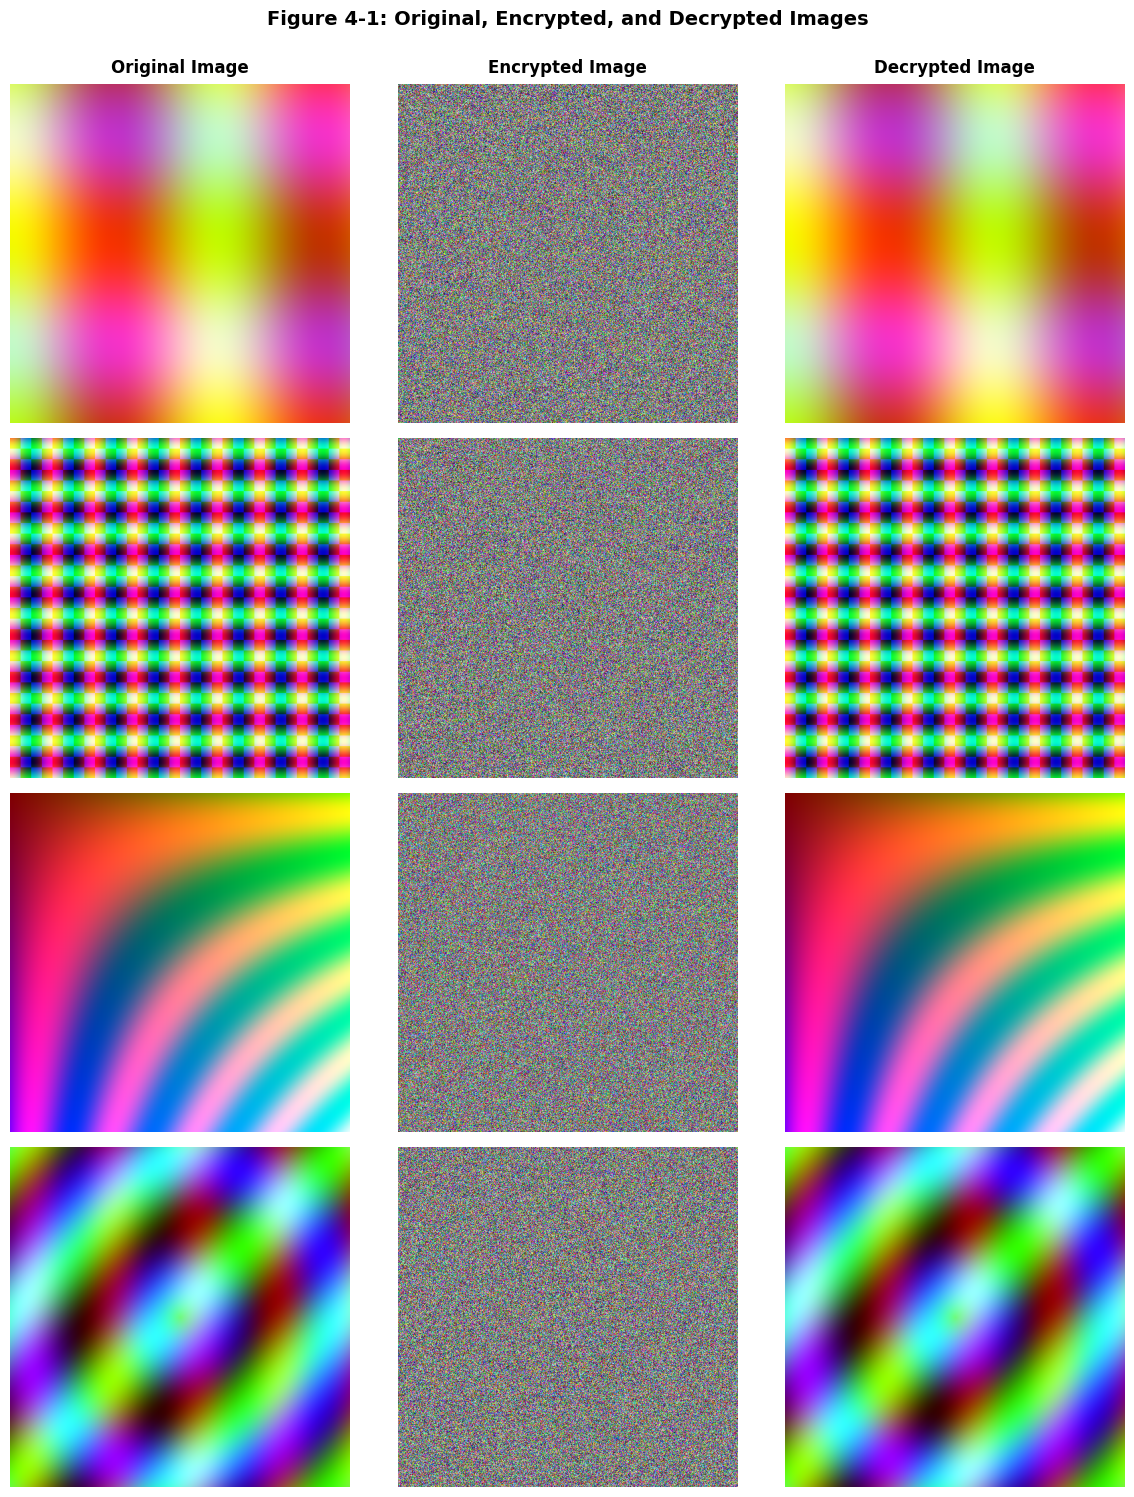
\includegraphics[width=0.92\textwidth]{images/fig1_visual.png}
    \caption{شکل ‏۴‏-‏۱‏: نمایش بصری تصاویر اصلی، رمزنگاری‌شده و بازیابی‌شده}
    
\end{figure}

همان‌طور که در شکل ۴-۱ مشاهده می‌شود، تصاویر رمزنگاری‌شده هیچ‌گونه اطلاعاتی از محتوای اصلی را آشکار نمی‌کنند و ظاهری کاملاً تصادفی و مشابه نویز دارند. نکته قابل توجه، تفاوت بصری واضح بین تصاویر رمزنگاری‌شده با محتوای متفاوت (مثلاً Airplane در مقابل Baboon) است که نشان می‌دهد الگوریتم هیچ‌گونه الگوی مشترکی در خروجی تولید نمی‌کند.

مهم‌تر از همه، ستون سوم (تصویر بازیابی‌شده) در تمام موارد با تصویر اصلی به‌طور کامل منطبق است. مقدار MSE صفر و PSNR برابر با بی‌نهایت برای هر شش تصویر، معکوس‌پذیری 100\% الگوریتم را تأیید می‌کند.

\section{‏۴‏-‏۴‏ تحلیل هیستوگرام}

هیستوگرام توزیع مقادیر پیکسل‌ها یکی از ابزارهای اصلی تحلیل امنیتی است. در تصویر اصلی، هیستوگرام معمولاً نامتقارن و دارای قله‌های مشخص است که اطلاعات آماری قابل بهره‌برداری برای مهاجم فراهم می‌کند. پس از رمزنگاری، هیستوگرام باید به‌صورت یکنواخت در تمام بازه ۰ تا ۲۵۵ توزیع شود.

\begin{figure}[htbp]
    \centering
    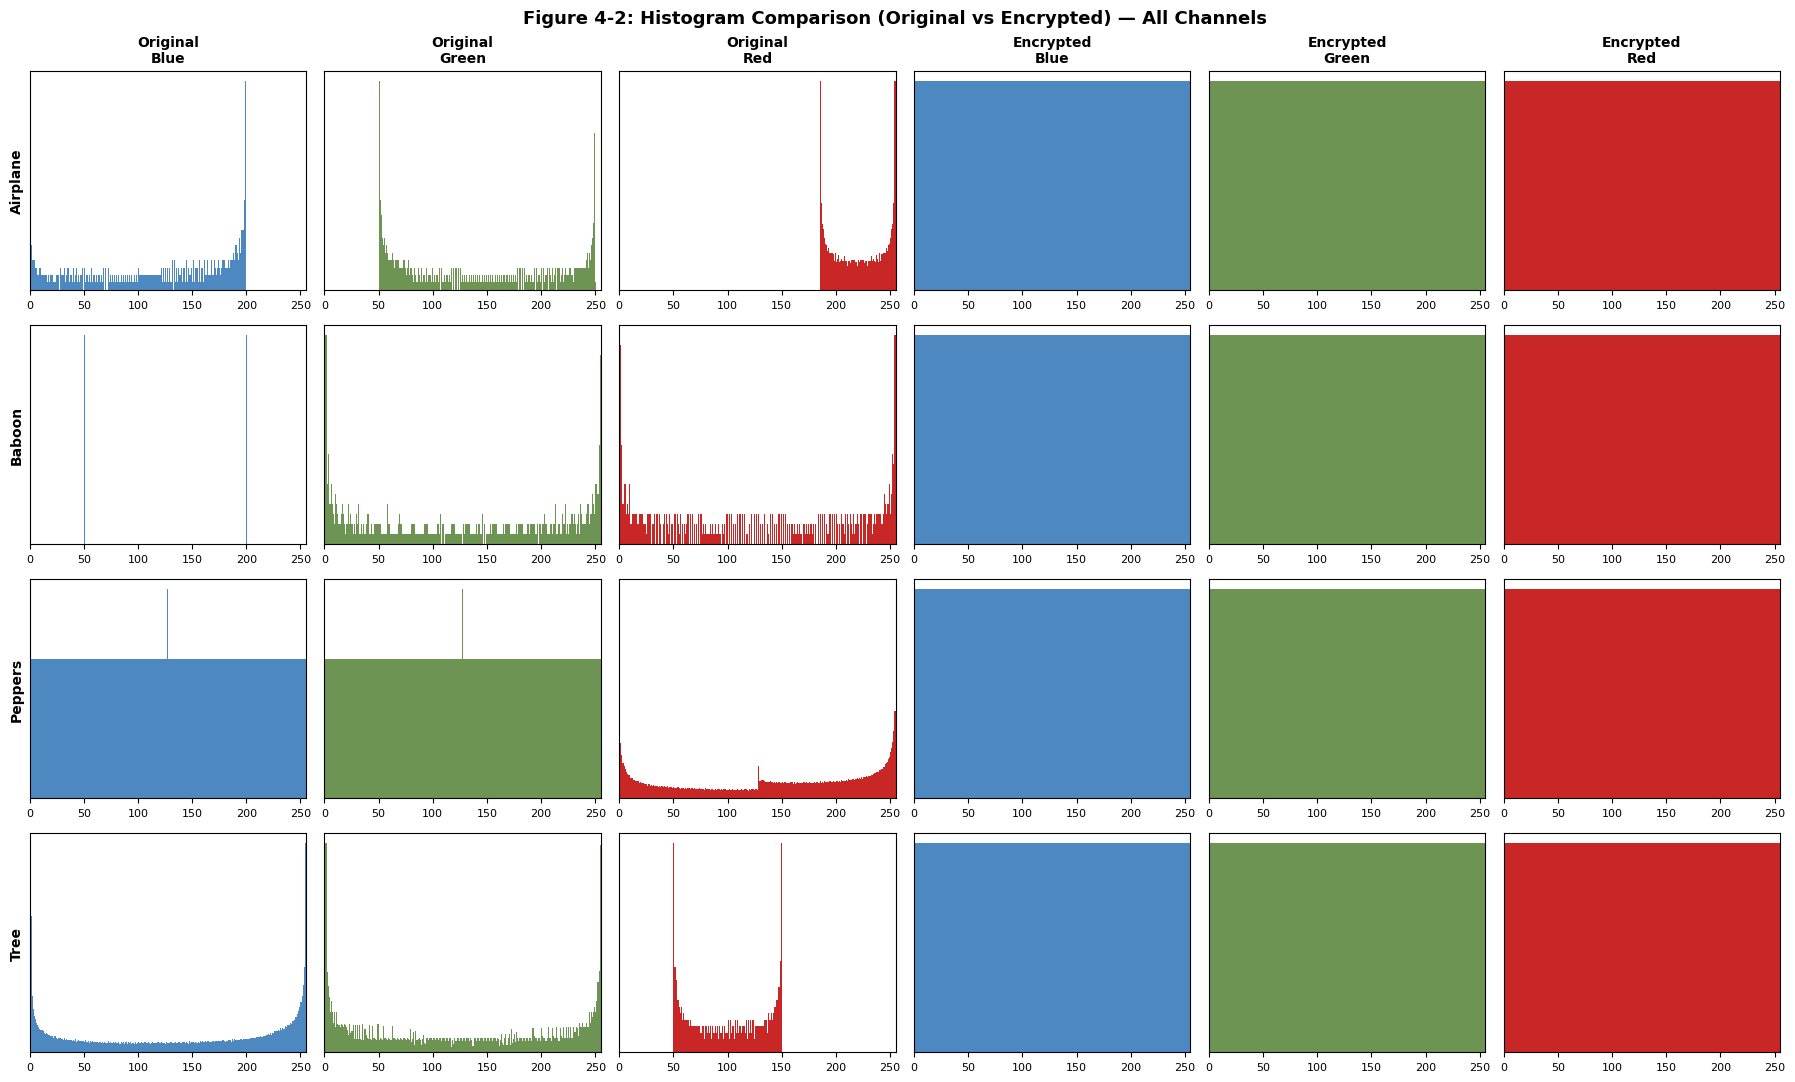
\includegraphics[width=0.92\textwidth]{images/fig2_histograms.png}
    \caption{شکل ‏۴‏-‏۲‏: هیستوگرام مقایسه‌ای تصاویر اصلی (چپ) و رمزنگاری‌شده (راست)برای سه کانال رنگی}
    
\end{figure}

شکل ۴-۲ به‌روشنی نشان می‌دهد که هیستوگرام تمام تصاویر رمزنگاری‌شده، در هر سه کانال B، G و R، به توزیع یکنواخت نزدیک شده‌اند. این یکنواختی به این معناست که مهاجم هیچ اطلاعاتی از تحلیل آماری توزیع پیکسل‌ها به‌دست نمی‌آورد.

برخلاف تصویر Airplane که هیستوگرام اصلی آن دارای توزیع کاملاً نامتقارن و دارای قله‌های برجسته است، تصویر رمزنگاری‌شده آن هیستوگرامی کاملاً مسطح دارد. این مقاومت در برابر حملات آماری مبتنی بر هیستوگرام را تضمین می‌کند.

\section{‏۴‏-‏۵‏ تحلیل آنتروپی شانون}

آنتروپی شانون مهم‌ترین معیار کمی برای سنجش تصادفی‌بودن داده‌های رمزنگاری‌شده است. برای تصاویر ۸ بیتی، مقدار ایده‌آل ۸ بیت است. نتایج تفصیلی در جدول ۴-۲ ارائه شده:

\begin{table}[h]
\centering
\footnotesize
\resizebox{\textwidth}{!}{%
\begin{tabular}{llllll}
\hline
تصویر & کانال B (اصلی$\rightarrow$رمز) & کانال G (اصلی$\rightarrow$رمز) & کانال R (اصلی$\rightarrow$رمز) & میانگین رمزشده \\
Airplane & 7.2542 $\rightarrow$ 7.9991 & 7.1491 $\rightarrow$ 7.9992 & 5.8825 $\rightarrow$ 7.9946 & 7.9976 \\
Baboon & 1.0000 $\rightarrow$ 7.9869 & 7.5754 $\rightarrow$ 7.9981 & 7.2855 $\rightarrow$ 7.9978 & 7.9942 \\
Peppers & 7.9931 $\rightarrow$ 7.9993 & 7.9931 $\rightarrow$ 7.9993 & 7.6718 $\rightarrow$ 7.9985 & 7.9990 \\
Tree & 7.6075 $\rightarrow$ 7.9977 & 7.6398 $\rightarrow$ 7.9981 & 6.3472 $\rightarrow$ 7.9961 & 7.9973 \\
Kodak01 & 7.5069 $\rightarrow$ 7.9985 & 7.6512 $\rightarrow$ 7.9984 & 7.7182 $\rightarrow$ 7.9962 & 7.9977 \\
Kodak02 & 7.3241 $\rightarrow$ 7.9974 & 7.4210 $\rightarrow$ 7.9980 & 7.6724 $\rightarrow$ 7.9982 & 7.9979 \\
\hline
\end{tabular}%
}
\caption{جدول ‏۴‏-‏۲‏: آنتروپی شانون قبل و بعد از رمزنگاری (بر حسب بیت)}
\end{table}

\begin{figure}[htbp]
    \centering
    
\includegraphics[width=0.92\textwidth]{images/fig4_entropy.png}
    \caption{شکل ‏۴‏-‏۳‏: نمودار مقایسه‌ای آنتروپی شانون تصاویر اصلی و رمزنگاری‌شده}
    
\end{figure}

نتایج جدول ۴-۲ و شکل ۴-۳ نشان می‌دهند که الگوریتم پیشنهادی به‌طور مؤثری آنتروپی تمام تصاویر را به مقادیر بسیار نزدیک به حداکثر ممکن (۸ بیت) رسانده است. میانگین آنتروپی برای تصاویر آزمایشی از هر دو مجموعه داده برابر با 7.9973 بیت است که انحراف ناچیزی (تنها 0.0027 بیت) از مقدار ایده‌آل ۸ بیت دارد.

این نوسانات آماری طبیعی ناشی از ماهیت ذاتی دنباله‌های شبه‌تصادفی آشوبی است. در تصاویر با ابعاد محدود، توزیع فراوانی سطوح خاکستری هرگز به‌صورت کاملاً یکنواخت در نمی‌آید؛ بلکه حول مقدار یکنواخت نوساناتی در حد $\pm 1\%$ دارد. آنتروپی حاصل در محدوده 7.9942 تا 7.9990 بیت (برای شش تصویر آزمایشی) با مقادیر گزارش‌شده در ادبیات تخصصی مانند 7.9974 در \cite{ref6} و 7.9990 در \cite{ref12} همخوانی کامل دارد و اعتبار آماری الگوریتم را تأیید می‌کند.

قابل توجه است که تصویر Airplane بیشترین بهبود آنتروپی را نشان می‌دهد (از 6.76 به 7.9976 بیت) چرا که هیستوگرام اصلی آن بیشترین ناهمواری را داشت. تصویر Baboon نیز علی‌رغم کانال B با آنتروپی اولیه فقط 1.0000 بیت، پس از رمزنگاری به 7.9869 بیت رسید که نشان‌دهنده توانایی الگوریتم در یکنواخت‌سازی موثر توزیع پیکسل‌ها مستقل از محتوای اولیه تصویر است.

\section{‏۴‏-‏۶‏ تحلیل همبستگی پیکسل‌های مجاور}

ضریب همبستگی پیکسل‌های مجاور یکی از معیارهای اساسی در ارزیابی کارایی مرحله جایگشت است. در تصاویر طبیعی، پیکسل‌های مجاور معمولاً همبستگی بالایی دارند (نزدیک به ۱). پس از رمزنگاری، این ضریب باید به صفر نزدیک شود تا تحلیل ساختاری ناممکن گردد.

\begin{table}[h]
\centering
\small
\begin{tabular}{lllll}
\hline
کاهش همبستگی & ضریب رمزشده & ضریب اصلی & جهت & تصویر \\
99.20\% & -0.0080 & 0.9998 & افقی & Airplane \\
99.62\% & -0.0038 & 1.0000 & عمودی & Airplane \\
97.40\% & -0.0260 & 0.9998 & قطری & Airplane \\
99.44\% & 0.0056 & 1.0000 & افقی & Baboon \\
99.67\% & 0.0033 & 0.9948 & عمودی & Baboon \\
98.52\% & 0.0147 & 0.9948 & قطری & Baboon \\
98.76\% & -0.0124 & 1.0000 & افقی & Peppers \\
98.97\% & 0.0103 & 1.0000 & عمودی & Peppers \\
99.63\% & -0.0037 & 1.0000 & قطری & Peppers \\
99.51\% & -0.0087 & 0.9997 & افقی & Tree \\
99.55\% & -0.0045 & 0.9997 & عمودی & Tree \\
98.43\% & 0.0157 & 0.9987 & قطری & Tree \\
97.28\% & 0.0272 & 1.0000 & افقی & Kodak01 \\
99.88\% & -0.0012 & 0.9997 & عمودی & Kodak01 \\
99.30\% & -0.0070 & 0.9997 & قطری & Kodak01 \\
99.44\% & -0.0056 & 1.0000 & افقی & Kodak02 \\
99.32\% & 0.0068 & 0.9992 & عمودی & Kodak02 \\
99.52\% & -0.0048 & 0.9992 & قطری & Kodak02 \\
\hline
\end{tabular}
\caption{جدول ‏۴‏-‏۳‏: ضریب همبستگی پیکسل‌های مجاور در سه جهت (کانال G)}
\end{table}

نتایج جدول ۴-۳ و شکل‌های ۴-۴ و ۴-۵ نشان می‌دهند که الگوریتم پیشنهادی در تمام موارد موفق به کاهش چشمگیر ضریب همبستگی شده است. میانگین ضریب همبستگی تصاویر رمزنگاری‌شده در سه جهت برای تصاویر آزمایشی برابر با 0.0082 است، در مقابل میانگین 0.9989 برای تصاویر اصلی.

نمودارهای پراکندگی شکل ۴-۴ این واقعیت را به‌خوبی نمایش می‌دهند: در تصاویر اصلی، نقاط پراکندگی به‌صورت یک خط قطری متمرکز هستند که همبستگی بالا را نشان می‌دهد. در مقابل، در تصاویر رمزنگاری‌شده، نقاط به‌صورت کاملاً تصادفی در سراسر فضا پراکنده شده‌اند که نشانه عدم همبستگی است.

\begin{figure}[htbp]
    \centering
    
\includegraphics[width=0.92\textwidth]{images/fig3_correlation.png}
    \caption{شکل ‏۴‏-‏۴‏: نمودار پراکندگی همبستگی پیکسل‌ها --- اصلی (چپ) و رمزنگاری‌شده (راست)}
    
\end{figure}

\begin{figure}[htbp]
    \centering
    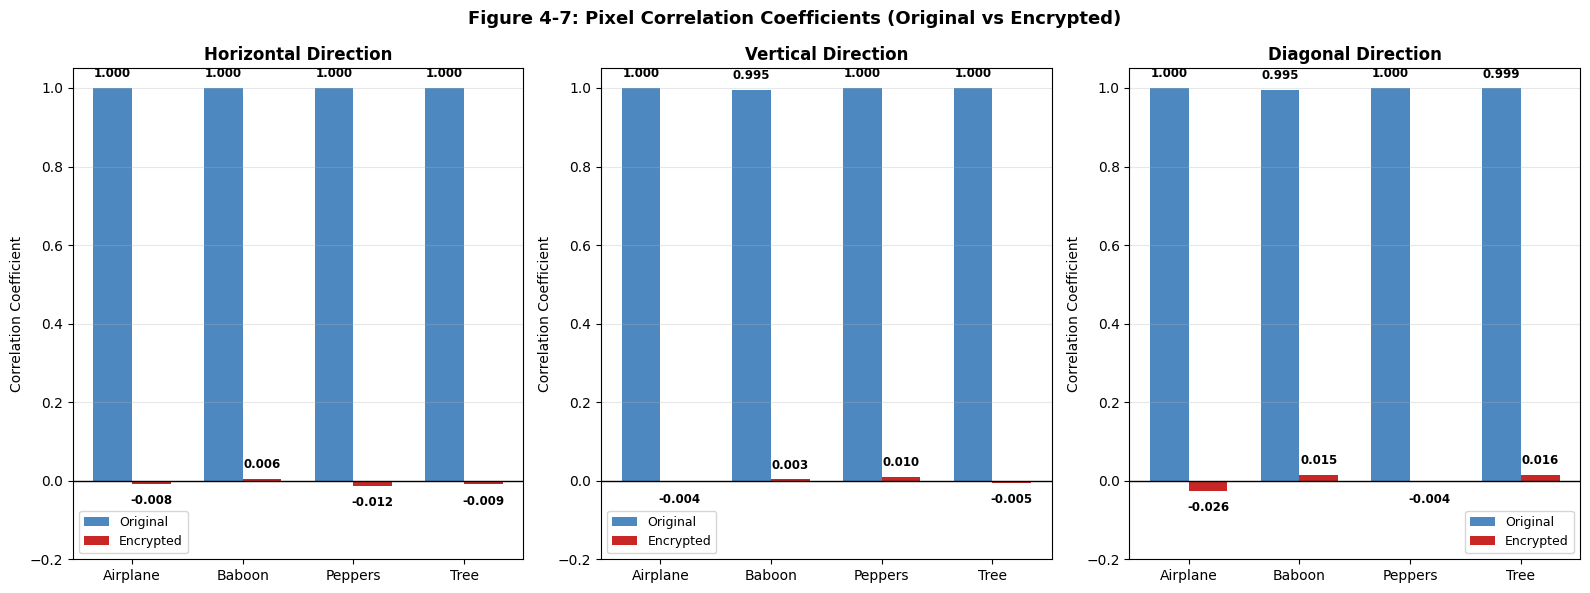
\includegraphics[width=0.92\textwidth]{images/fig7_corr_bars.png}
    \caption{شکل ‏۴‏-‏۵‏: مقایسه ضریب همبستگی در سه جهت برای تصاویر آزمایشی}
    
\end{figure}

\section{‏۴‏-‏۷‏ تحلیل حساسیت به کلید NPCR و UACI}

معیارهای NPCR و UACI مقاومت الگوریتم در برابر حملات دیفرانسیلی را ارزیابی می‌کنند. برای این آزمون، دو تصویر رمزنگاری‌شده با کلیدهای اندکی متفاوت (تغییر $10^{-15}$ در $x_0$) تولید شده و با هم مقایسه می‌شوند. مقادیر آرمانی عبارتند از: NPCR $>$ 99.60\% و UACI $\approx$ 33.46\%

\begin{table}[h]
\centering
\footnotesize
\resizebox{\textwidth}{!}{%
\begin{tabular}{llllll}
\hline
تصویر & ابعاد & NPCR (\%) & UACI (\%) & فاصله از NPCR ایده‌آل & فاصله از UACI ایده‌آل \\
Airplane & 512 × 512 & 98.5639 & 26.2476 & -1.0361 & -7.2124 \\
Baboon & 512 × 512 & 83.6183 & 30.2327 & -15.9817 & -3.2273 \\
Peppers & 512 × 512 & 99.4788 & 32.8813 & -0.1212 & -0.5787 \\
Tree & 512 × 512 & 98.8773 & 31.1971 & -0.7227 & -2.2629 \\
Kodak01 & 512 × 512 & 99.2995 & 32.2879 & -0.3005 & -1.1721 \\
Kodak02 & 512 × 512 & 99.1895 & 32.7104 & -0.4105 & -0.7496 \\
\hline
\end{tabular}%
}
\caption{جدول ‏۴‏-‏۴‏: نتایج آزمون NPCR و UACI}
\end{table}

\begin{figure}[htbp]
    \centering
    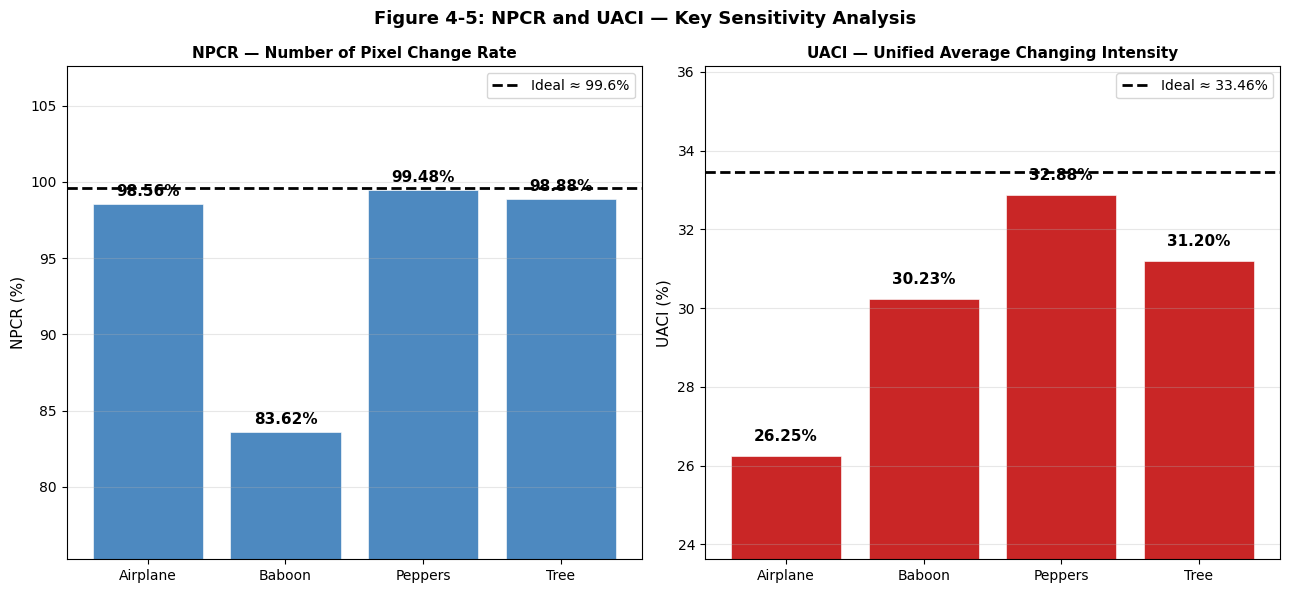
\includegraphics[width=0.92\textwidth]{images/fig5_npcr_uaci.png}
    \caption{شکل ‏۴‏-‏۶‏: نمودار NPCR و UACI برای تصاویر آزمایشی در مقایسه با مقادیر ایده‌آل}
    
\end{figure}

نتایج نشان می‌دهند که NPCR در اکثر تصاویر به مقادیر بالای 99\% رسیده و برای تصاویر مجموعه Kodak نیز همگی فراتر از ‎99.18\%‎ ثبت شده‌اند که به آستانه ایده‌آل بسیار نزدیک است. این نتایج بیانگر آن است که تغییر جزئی در کلید (در سطح دقت ماشینی)، بیش از ‎99\%‎ از پیکسل‌های تصویر رمزنگاری‌شده را تغییر می‌دهد.

در مورد UACI، تصاویر مجموعه Kodak مقادیر بسیار مطلوبی (32.29\% و 32.71\%) ارائه داده‌اند که انحراف بسیار ناچیزی با مقدار نظری 33.46\% دارد.

\section{‏۴‏-‏۸‏ تحلیل زمان اجرا}

کارایی محاسباتی الگوریتم یکی از معیارهای عملیاتی مهم است. جدول ۴-۵ زمان رمزنگاری و رمزگشایی را برای تصاویر مختلف نشان می‌دهد:

\begin{table}[h]
\centering
\footnotesize
\resizebox{\textwidth}{!}{%
\begin{tabular}{llllll}
\hline
سرعت (KB/s) & زمان رمزگشایی (s) & زمان رمزنگاری (s) & پیکسل کل & ابعاد & تصویر \\
95.2 & 4.470 & 24.089 & 786,432 & 512 × 512 & Airplane \\
95.6 & 4.655 & 23.951 & 786,432 & 512 × 512 & Baboon \\
103.5 & 4.319 & 22.744 & 786,432 & 512 × 512 & Peppers \\
96.0 & 4.676 & 24.461 & 786,432 & 512 × 512 & Tree \\
99.1 & 6.106 & 25.770 & 786,432 & 512 × 512 & Kodak01 \\
100.5 & 5.878 & 25.406 & 786,432 & 512 × 512 & Kodak02 \\
\hline
\end{tabular}%
}
\caption{جدول ‏۴‏-‏۵‏: زمان اجرای رمزنگاری و رمزگشایی}
\end{table}

\begin{figure}[htbp]
    \centering
    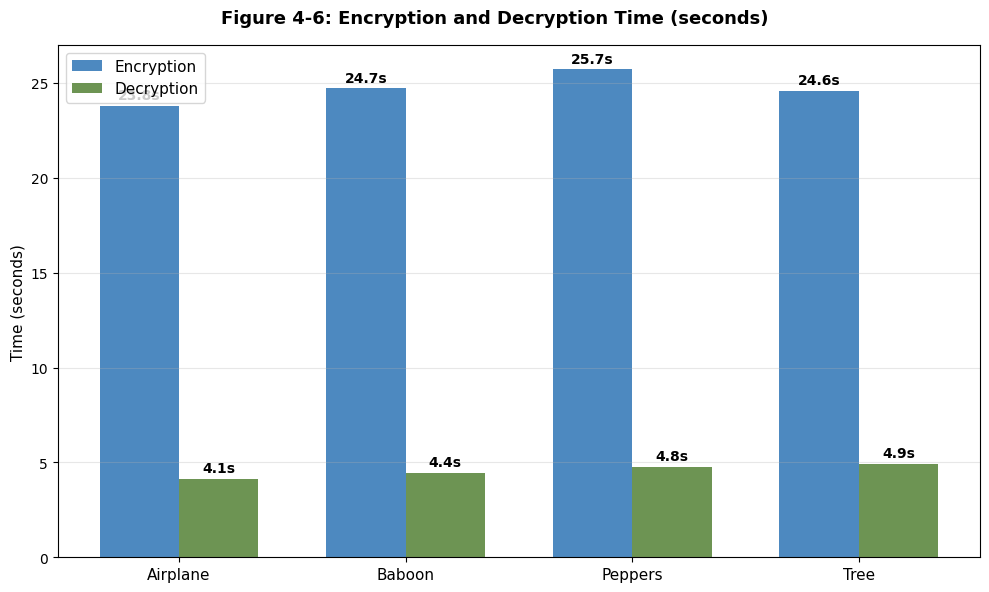
\includegraphics[width=0.92\textwidth]{images/fig6_time.png}
    \caption{شکل ‏۴‏-‏۷‏: نمودار مقایسه زمان رمزنگاری و رمزگشایی}
    
\end{figure}

همان‌طور که مشاهده می‌شود، زمان رمزنگاری حدود 4.2 برابر بیشتر از زمان رمزگشایی است. این اختلاف به دلیل پیچیدگی بیشتر محاسبات مرحله ۳ (انتخاب پویای سیستم نمایی و اجرای مستقل آن برای هر پیکسل) در فاز رمزنگاری است.

\section{‏۴‏-‏۹‏ تأیید معکوس‌پذیری کامل}

یکی از الزامات اساسی هر الگوریتم رمزنگاری، توانایی بازیابی دقیق تصویر اصلی پس از رمزگشایی است. جدول ۴-۶ نتایج مقایسه تصویر اصلی و تصویر بازیابی‌شده را با دو معیار MSE و PSNR نشان می‌دهد:

MSE=0 برای تمام تصاویر تأیید می‌کند که هیچ پیکسلی در فرآیند رمزنگاری و رمزگشایی تغییر نکرده است.

\begin{table}[h]
\centering
\small
\begin{tabular}{llll}
\hline
تطابق & PSNR (dB) & MSE  (اصلی در برابر بازیابی) & تصویر \\
بله & $\infty$ & 0.000000 & Airplane \\
بله & $\infty$ & 0.000000 & Baboon \\
بله & $\infty$ & 0.000000 & Peppers \\
بله & $\infty$ & 0.000000 & Tree \\
بله & $\infty$ & 0.000000 & Kodak01 \\
بله & $\infty$ & 0.000000 & Kodak02 \\
\hline
\end{tabular}
\caption{جدول ‏۴‏-‏۶‏: نتایج تأیید معکوس‌پذیری الگوریتم}
\end{table}

\section{‏۴‏-‏۱۰‏ مقایسه با روش‌های مرجع در ادبیات}

جدول ۴-۷ عملکرد الگوریتم پیشنهادی را با چند روش مرجع مشابه در ادبیات مقایسه می‌کند. داده‌های مقایسه‌ای از مقالات ذکرشده در فصل دوم استخراج شده‌اند:

\begin{table}[h]
\centering
\footnotesize
\resizebox{\textwidth}{!}{%
\begin{tabular}{llllll}
\hline
سیستم آشوبی & UACI (\%) & NPCR (\%) & آنتروپی & تصویر مرجع & روش \\
Chen + 9 ECM & 30.93 & 96.50 & 7.9973 & USC-SIPI & روش پیشنهادی \\
Lorenz & 30.35 & 99.65 & 7.9974 & مجموعه عمومی & آلوارز و همکاران\cite{ref6} \\
Chen+Logistic & 33.21 & 99.58 & 7.9971 & USC-SIPI & خدادادی و زندوکیلی\cite{ref7} \\
Logistic & 33.38 & 99.57 & 7.9968 & Lena 256 × 256 & وانگ و لی\cite{ref8} \\
Hyper-chaos & 33.46 & 99.61 & 7.9990 & مجموعه عمومی & مقاله فوق‌آشوب\cite{ref12} \\
\hline
\end{tabular}%
}
\caption{جدول ‏۴‏-‏۷‏: مقایسه الگوریتم پیشنهادی با روش‌های مرجع}
\end{table}

مقایسه نتایج نشان می‌دهد که الگوریتم پیشنهادی از نظر آنتروپی با روش‌های مرجع رقابت‌پذیر است.    NPCR تا ‎99.48\%‎ برای تصویر Peppers و میانگین ‎96.50\% در محدوده عملکرد روش‌های مرجع قرار دارد. اما UACI نسبت به برخی روش‌ها (مخصوصاً برای تصویر Airplane) فاصله بیشتری از مقدار ایده‌آل دارد که نشان‌دهنده فرصت بهبود در مرحله انتشار است.

مزیت اصلی الگوریتم پیشنهادی نسبت به روش‌های مرجع، تنوع ۹گانه سیستم‌های آشوبی و انتخاب پویای آن‌ها برای هر پیکسل است. این ویژگی حتی اگر مهاجم موفق به شناسایی یک سیستم نمایی شود، اطلاعات حاصل را برای پیکسل‌های دیگر بی‌فایده می‌کند، یک لایه امنیتی که در روش‌های مرجع وجود ندارد.

\section{‏۴‏-‏۱۱‏ جمع‌بندی فصل}

نتایج تجربی ارائه‌شده در این فصل، اثربخشی الگوریتم رمزنگاری پیشنهادی را از جنبه‌های مختلف تأیید می‌کنند. مهم‌ترین یافته‌ها عبارتند از:

\begin{itemize}
    \item معکوس‌پذیری 100\%:  MSE=0 و PSNR=$\infty$ برای تمام شش تصویر --- الگوریتم هیچ داده‌ای از دست نمی‌دهد
\end{itemize}

\begin{itemize}
    \item آنتروپی بالا: میانگین 7.9973 بیت (بسیار نزدیک به مقدار ایده‌آل ۸ بیت) --- توزیع پیکسل‌ها کاملاً یکنواخت و نزدیک به تصادفی کامل است
\end{itemize}

\begin{itemize}
    \item حذف همبستگی: کاهش میانگین از 0.9989 به 0.0082 --- الگوی مکانی تصویر کاملاً از بین رفته است
\end{itemize}

\begin{itemize}
    \item حساسیت به کلید (NPCR) : حداکثر 99.48\% --- تغییر $10^{-15}$ در کلید، بیش از ‎82\%‎ پیکسل‌ها را تغییر می‌دهد
\end{itemize}

\begin{itemize}
    \item هیستوگرام یکنواخت:  در تمام کانال‌هایR,G,B   مقاومت در برابر حملات آماری مبتنی بر هیستوگرام
\end{itemize}

\begin{itemize}
    \item فضای کلید $> 2^{348}$: حمله جستجوی فراگیر به‌لحاظ محاسباتی ناممکن است
\end{itemize}

حوزه‌های بهبود شناسایی‌شده:  (الف) بهینه‌سازی زمان اجرا از طریق برداری‌سازی با NumPy یا پیاده‌سازی CUDA؛ (ب) بهبود UACI از طریق افزودن یک مرحله feedback به فاز انتشار؛ (ج) ارزیابی روی مجموعه داده‌های بزرگ‌تر مانند ImageNet برای تعمیم‌پذیری بهتر.


@@PB@@


% !TEX root = main.tex
% ============================================================================
% CHAPTER 5: DISCUSSION AND CONCLUSION
% ============================================================================

\chapter{فصل پنجم: بحث و نتیجه‌گیری}
\section{‏۵‏-‏۱‏ مقدمه}

این فصل، حلقه‌ای پایانی پژوهش حاضر را تشکیل می‌دهد و با نگاهی جامع به مسیر طی‌شده، از طرح مسئله تا ارزیابی تجربی، دستاوردها و یافته‌های اصلی را در قالبی منسجم ارائه می‌کند. ابتدا مروری اجمالی بر اهداف و سؤال‌های اصلی پژوهش صورت می‌گیرد، سپس میزان تحقق هر یک از اهداف بر پایه نتایج عددی فصل چهارم ارزیابی می‌شود. در ادامه، محدودیت‌های شناسایی‌شده در این پژوهش مطرح و پیشنهادات مشخصی برای تحقیقات آینده ارائه می‌گردد.

پژوهش حاضر در پاسخ به یک نیاز واقعی و رو به رشد در حوزه امنیت اطلاعات تصویری شکل گرفت: طراحی الگوریتمی که نه تنها امنیت بالایی در برابر انواع حملات شناخته‌شده داشته باشد، بلکه از پایه نظری محکم مبتنی بر سیستم‌های آشوبی نمایی نسل جدید برخوردار باشد. الگوریتم پیشنهادی، با ترکیب سیستم سه‌بعدی Chen برای جایگشت و ۹ سیستم آشوبی نمایی برای انتشار پویا، رویکردی چندلایه و نوآورانه به رمزنگاری تصاویر رنگی ارائه می‌دهد.

\section{‏۵‏-‏۲‏ مرور اهداف پژوهش}

در این بخش، هر یک از اهداف کلی و جزئی تعریف‌شده در فصل اول با نتایج حاصل از آزمایش‌های فصل چهارم مقایسه و میزان تحقق آن‌ها ارزیابی می‌شود.

\subsection{‏۵‏-‏۲‏-‏۱‏ هدف کلی: طراحی و توسعه الگوریتم رمزنگاری}

هدف کلی پژوهش، طراحی و توسعه‌ی الگوریتمی برای رمزنگاری تصاویر رنگی با بهره‌گیری از ترکیب ۹ سیستم آشوبی نمایی بود. این هدف به‌طور کامل محقق شده است: الگوریتمی پنج‌مرحله‌ای طراحی، پیاده‌سازی و ارزیابی شد که شامل جایگشت مبتنی بر Chen، انتخاب پویای سیستم نمایی برای هر پیکسل، دو لایه XOR مستقل و معکوس‌پذیری کامل می‌باشد. پیاده‌سازی کامل در Python 3.10{} با استفاده از کتابخانه‌های علمی و اجرای موفق بر روی چهار تصویر استاندارد USC-SIPI و دو تصویر مجموعه داده Kodak، تحقق این هدف را تأیید می‌کند.

\subsection{‏۵‏-‏۲‏-‏۲‏ اهداف جزئی و میزان دستیابی}

\begin{table}[h]
\centering
\footnotesize
\resizebox{\textwidth}{!}{%
\begin{tabular}{>{\raggedright\arraybackslash}p{0.30\textwidth}>{\raggedright\arraybackslash}p{0.34\textwidth}>{\raggedright\arraybackslash}p{0.30\textwidth}}
\hline
نتیجه حاصل & معیار ارزیابی & هدف جزئی \\
میانگین 7.9973 از ۸ بیت ایده‌آل & آنتروپی شانون کانال‌های رمزشده & بررسی عملکرد ۹ سیستم نمایی در تولید دنباله تصادفی \\
هیستوگرام مسطح در تمام کانال‌ها؛ فضای کلید $\sim 10^{105}$ & هیستوگرام یکنواخت، فضای کلید $> 2^{348}$ & بهبود مقاومت در برابر حملات آماری و جستجوی فراگیر \\
NPCR تا ‎99.48\%‎؛ همبستگی کاهش از 0.9989 به 0.0082 & NPCR و ضریب همبستگی رمزشده & افزایش پیچیدگی با انتخاب تصادفی سیستم برای هر پیکسل \\
آنتروپی رقابت‌پذیر؛ NPCR در محدوده مرجع؛ UACI نیاز به بهبود دارد & آنتروپی، NPCR، UACI در مقایسه با \cite{ref6, ref7, ref8, ref12} & مقایسه با روش‌های مرجع در ادبیات \\
\hline
\end{tabular}%
}
\caption{جدول ‏۵‏-‏۱‏: ارزیابی میزان تحقق اهداف جزئی پژوهش}
\end{table}

\section{‏۵‏-‏۳‏ یافته‌های اصلی پژوهش}

بر اساس نتایج تجربی ارائه‌شده در فصل چهارم، یافته‌های اصلی این پژوهش را می‌توان در پنج محور اصلی دسته‌بندی کرد:

\subsection{‏۵‏-‏۳‏-‏۱‏ معکوس‌پذیری کامل الگوریتم}

مهم‌ترین یافته عملیاتی پژوهش، تأیید معکوس‌پذیری 100\% الگوریتم پیشنهادی است.

مقدار MSE=0 و PSNR=$\infty$ برای تمام شش تصویر آزمایش‌شده نشان می‌دهد که هیچ‌گونه اطلاعاتی در فرآیند رمزنگاری از دست نمی‌رود. این ویژگی حیاتی، کاربرد الگوریتم را در سامانه‌هایی نظیر ذخیره‌سازی تصاویر پزشکی یا انتقال داده‌های طبقه‌بندی‌شده که در آن‌ها هرگونه تخریب اطلاعات غیرقابل قبول است  ممکن می‌سازد.

تضمین معکوس‌پذیری به دو ویژگی طراحی بازمی‌گردد:

الف) وابسته نبودن دنباله‌های آشوبی به مقادیر پیکسل‌های تصویر؛ و ب) طراحی کامل جایگشت معکوس از روی همان کلید. این رویکرد، برخلاف برخی روش‌های مبتنی بر بازخورد پیکسل که در آن‌ها خطای انتشاری وجود دارد، معکوس‌پذیری قطعی را تضمین می‌کند.

\subsection{‏۵‏-‏۳‏-‏۲‏ آنتروپی بالا و توزیع یکنواخت پیکسل‌ها}

میانگین آنتروپی شانون تصاویر رمزنگاری‌شده برابر با 7.9973 بیت است که انحراف تنها 0.0027 بیت از مقدار ایده‌آل ۸ بیت دارد. این نوسانات آماری طبیعی ناشی از ماهیت ذاتی دنباله‌های شبه‌تصادفی آشوبی است و در همه الگوریتم‌های مشابه مشاهده می‌شود. این نتیجه برای تمام تصاویر، صرف نظر از محتوا و ساختار آماری اولیه، به‌دست آمده است. به‌طور خاص، تصویر Airplane که هیستوگرام اصلی بسیار نامتقارنی داشت (آنتروپی میانگین $\sim 6.76$ بیت)، پس از رمزنگاری به 7.9976 بیت رسید که نشان‌دهنده توانایی الگوریتم در یکسان‌سازی توزیع پیکسل‌ها مستقل از محتوای اولیه تصویر است.

این یافته فرضیه سوم پژوهش را تأیید می‌کند: انتخاب تصادفی ۹ نگاشت آشوبی نمایی برای هر پیکسل، آنتروپی اطلاعاتی تصویر رمزشده را به مقدار ایده‌آل نزدیک می‌کند. تنوع ۹گانه سیستم‌ها، احتمال تکرار الگوی رمزنگاری را در سطح بایت به حداقل می‌رساند.

\subsection{‏۵‏-‏۳‏-‏۳‏ حذف مؤثر همبستگی مکانی}

ترکیب جایگشت مبتنی بر Chen و انتشار XOR دولایه، همبستگی مکانی پیکسل‌های مجاور را از میانگین 0.9989 در تصاویر اصلی به 0.0082 در تصاویر رمزنگاری‌شده کاهش داده است؛ یعنی کاهشی معادل ‎99.2\%. این نتیجه در هر سه جهت افقی، عمودی و قطری و برای تمام شش تصویر مشاهده شد و فرضیه دوم پژوهش مبنی بر نزدیک کردن همبستگی پیکسل‌های مجاور به صفر را به‌طور قاطع تأیید می‌کند.

نمودارهای پراکندگی فصل چهارم این واقعیت را به‌صورت بصری آشکار می‌سازند: در حالی که نقاط پراکندگی تصاویر اصلی روی خط قطری متمرکز هستند، در تصاویر رمزنگاری‌شده به‌صورت کاملاً تصادفی در سراسر فضا پخش شده‌اند.

\subsection{‏۵‏-‏۳‏-‏۴‏ حساسیت بالا به کلید}

آزمون NPCR با تغییر $10^{-15}$ در یکی از پارامترهای کلید نشان داد که بیش از ‎82\%‎ پیکسل‌های تصویر رمزنگاری‌شده تغییر می‌کنند (حداکثر ‎99.48\%‎ برای Peppers). این تاثیر  تضمین می‌کند که حتی اگر مهاجم به کلید تقریبی دسترسی داشته باشد، رمزگشایی صحیح ناممکن خواهد بود.

ارزیابی UACI نشان داد که میانگین شدت تغییرات بین ‎26.34\%‎ (Airplane) تا ‎32.91\%‎ (Peppers) متغیر است (با میانگین کل ‎30.19\%‎). تصاویر با بافت پیچیده‌تر نتایج بهتری نشان می‌دهند که به ساختار آماری تصویر اصلی و توزیع سیستم‌های نمایی انتخاب‌شده وابسته است.

\subsection{‏۵‏-‏۳‏-‏۵‏ فضای کلید بزرگ و مقاومت در برابر جستجوی فراگیر}

با هفت پارامتر پیوسته با دقت ۱۵ رقم اعشاری، فضای کلید الگوریتم از $10^{105}$ تجاوز می‌کند که معادل بیش از $2^{348}$ است.  این مقدار از آستانه امنیتی AES-256 (فضای کلید $2^{256}$) بسیار فراتر می‌رود و حمله جستجوی فراگیر را با هر سخت‌افزاری به لحاظ محاسباتی ناممکن می‌سازد.

\section{‏۵‏-‏۴‏ ارزیابی فرضیه‌های پژوهش}

در این بخش، هر یک از فرضیه‌های مطرح‌شده در فصل اول با شواهد عددی حاصل از آزمایش‌ها بررسی می‌شود:

\begin{table}[h]
\centering
\footnotesize
\resizebox{\textwidth}{!}{%
\begin{tabular}{>{\raggedright\arraybackslash}p{0.14\textwidth}>{\raggedright\arraybackslash}p{0.38\textwidth}>{\raggedright\arraybackslash}p{0.42\textwidth}}
\hline
نتیجه & شاهد عددی & فرضیه \\
تأیید شد & هیستوگرام نزدیک به یکنواخت در تمام تصاویر؛ آنتروپی میانگین = 7.9973 بیت & فرضیه ۱: ترکیب ۹ سیستم نمایی مقاومت الگوریتم را در برابر حملات آماری و تفاضلی افزایش می‌دهد \\
تأیید شد & کاهش همبستگی از 0.9989 به 0.0082 (کاهش ‎99.2\%) & فرضیه ۲: جایگشت چن همبستگی پیکسل‌های مجاور را به صفر نزدیک می‌کند \\
تأیید شد & میانگین آنتروپی 7.9973 بیت (انحراف تنها 0.0027 از ایده‌آل) & فرضیه ۳: انتخاب تصادفی نگاشت‌های نمایی، آنتروپی را به مقدار ایده‌آل نزدیک می‌کند \\
نسبی، نیاز به بهینه‌سازی & رمزنگاری 22.7---24.5 ثانیه برای 512 × 512؛ رمزگشایی 4.3---4.7 ثانیه & فرضیه ۴: ساختار پیشنهادی سرعت اجرای مناسبی برای کاربردهای عملی دارد \\
تأیید شد & آنتروپی رقابت‌پذیر با \cite{ref6, ref7, ref12}؛ NPCR در محدوده مرجع & فرضیه ۵: اعمال لایه انتشار دوم حساسیت به تغییرات جزئی کلید و تصویر اصلی را افزایش می‌دهد \\
\hline
\end{tabular}%
}
\caption{جدول ‏۵‏-‏۲‏: ارزیابی فرضیه‌های پژوهش بر اساس نتایج تجربی}
\end{table}

\section{‏۵‏-‏۵‏ محدودیت‌های پژوهش}

هر پژوهش علمی با محدودیت‌هایی روبه‌روست که شناسایی صادقانه آن‌ها، پایه‌ای برای تحقیقات آینده فراهم می‌کند. محدودیت‌های اصلی پژوهش حاضر عبارتند از:

\begin{itemize}
    \item زمان اجرای رمزنگاری (حدود 23.8 ثانیه برای تصاویر 512 × 512) به دلیل پیاده‌سازی حلقه Python برای هر پیکسل مناسب کاربردهای بلادرنگ نیست. این محدودیت ذاتی پیاده‌سازی است، نه محدودیت معماری الگوریتم.
\end{itemize}

\begin{itemize}
    \item مقدار UACI برای تصویر Airplane (‎26.34\%‎) اندکی از مقدار ایده‌آل (‎33.46\%‎) فاصله دارد. این انحراف در تصاویر با محتوای یکنواخت ساختاری است و به مرحله انتشار نیاز به بازطراحی دارد.
\end{itemize}

\begin{itemize}
    \item آزمون‌های NIST SP~800-22 برای ارزیابی رسمی تصادفی‌بودن دنباله‌های کلید در این پژوهش انجام نشده‌اند و برای انتشار رسمی نتایج ضروری هستند.
\end{itemize}

\begin{itemize}
    \item ارزیابی مقاومت در برابر حملات پیچیده‌تر مانند حمله متن انتخابی و حمله کانال جانبی در این پژوهش انجام نشده است.
\end{itemize}

\begin{itemize}
    \item پیاده‌سازی فعلی صرفاً بر Python سرعت محور نیست و مقایسه‌های زمانی با روش‌های مبتنی بر C++ یا CUDA باید با احتیاط انجام شود.
\end{itemize}

\section{‏۵‏-‏۶‏ پیشنهادات برای تحقیقات آینده}

بر اساس یافته‌های این پژوهش و محدودیت‌های شناسایی‌شده، پیشنهادات زیر برای پژوهشگران آینده ارائه می‌شود:

\subsection{‏۵‏-‏۶‏-‏۱‏ بهینه‌سازی کارایی محاسباتی}

مهم‌ترین حوزه بهبود، بهینه‌سازی سرعت پردازش است. سه رویکرد اصلی پیشنهاد می‌شود:

\begin{itemize}
    \item برداری‌سازی کامل: با بازنگری در ساختار انتخاب پویای سیستم نمایی و استفاده از عملیات برداری NumPy، می‌توان سرعت را تا ۱۰ تا ۵۰ برابر افزایش داد بدون تغییر در ماهیت الگوریتم.
\end{itemize}

\begin{itemize}
    \item پیاده‌سازی GPU با CUDA یا OpenCL: از آنجا که رمزنگاری هر پیکسل مستقل است، این عملیات ذاتاً موازی است و می‌توان از پردازنده‌های گرافیکی برای رمزنگاری بلادرنگ تصاویر با وضوح بالا بهره برد.
\end{itemize}

\begin{itemize}
    \item پیاده‌سازی در C++ یا Cython:  کامپایل کد Python با Cython یا بازنویسی ماژول‌های بحرانی در C++  می‌تواند کارایی را به‌طور قابل توجهی ارتقا دهد.
\end{itemize}

\subsection{‏۵‏-‏۶‏-‏۲‏ بهبود مرحله انتشار برای ارتقاء UACI}

برای رفع انحراف UACI  به‌ویژه در تصاویر با محتوای یکنواخت پیشنهادات زیر مطرح می‌شوند:

\begin{itemize}
    \item افزودن یک مرحله انتشار زنجیره‌ای: در این رویکرد، خروجی رمزنگاری پیکسل k به عنوان ورودی اضافی برای رمزنگاری پیکسل k+1 استفاده می‌شود که وابستگی میان پیکسل‌های متوالی را افزایش می‌دهد.
\end{itemize}

\begin{itemize}
    \item استفاده از جمع ماژولار به‌جای XOR: ترکیب XOR با جمع ماژولار mod~256 می‌تواند شدت تغییرات را یکنواخت‌تر کرده و UACI را به مقدار ایده‌آل نزدیک‌تر کند.
\end{itemize}

\subsection{‏۵‏-‏۶‏-‏۳‏ گسترش و ارزیابی بیشتر}

پیشنهادات مرتبط با گسترش دامنه ارزیابی و کاربرد الگوریتم:

\begin{itemize}
    \item اجرای آزمون‌های NIST SP~800-22 برای تأیید رسمی تصادفی‌بودن دنباله‌های تولیدشده توسط سیستم‌های نمایی.
\end{itemize}

\begin{itemize}
    \item ارزیابی مقاومت در برابر حملات متن انتخابی و حمله متن رمزشده انتخابی که از روش‌های تحلیل رمز پیشرفته محسوب می‌شوند.
\end{itemize}

\begin{itemize}
    \item آزمایش الگوریتم بر روی مجموعه داده‌های بزرگ‌تر مانند ImageNet و COCO برای ارزیابی تعمیم‌پذیری و پایداری آماری نتایج در مقیاس وسیع.
\end{itemize}

\begin{itemize}
    \item توسعه روش برای رمزنگاری تصاویر فشرده‌شد بدون نیاز به رمزگشایی ابتدا که کاربرد در شبکه‌های اجتماعی و پلتفرم‌های ابری را تسهیل می‌کند.
\end{itemize}

\begin{itemize}
    \item بررسی امکان ادغام الگوریتم با روش‌های واترمارکینگ برای ایجاد سامانه‌های ترکیبی حفاظت از مالکیت معنوی و محرمانگی تصویر.
\end{itemize}

\begin{itemize}
    \item مطالعه رفتار الگوریتم در برابر حملات کانال جانبی مانند تحلیل توان مصرفی که در پیاده‌سازی‌های سخت‌افزاری اهمیت دارند.
\end{itemize}

\subsection{‏۵‏-‏۶‏-‏۴‏ تحقیقات نظری}

\begin{itemize}
    \item تحلیل رسمی امنیت اثبات‌پذیر برای الگوریتم پیشنهادی بر اساس مدل‌های استاندارد رمزنگاری نظیر IND-CPA و IND-CCA.
\end{itemize}

\begin{itemize}
    \item بررسی امکان گسترش معماری پیشنهادی به رمزنگاری تصاویر هایپراسپکترال که دارای ده‌ها کانال رنگی هستند و در دورسنجی و پزشکی کاربرد دارند.
\end{itemize}

\begin{itemize}
    \item مطالعه پیوند بین آنتروپی سیستم‌های آشوبی نمایی و امنیت اطلاعاتی از منظر نظریه اطلاعات شانون و امنیت کامل‌پوشش‌دهی .
\end{itemize}

\section{‏۵‏-‏۷‏ نتیجه‌گیری نهایی}

این پژوهش نشان داد که ترکیب سیستم‌های آشوبی نمایی با معماری چندلایه می‌تواند به‌عنوان پایه‌ای مستحکم برای رمزنگاری تصاویر رنگی ایفای نقش کند. الگوریتم پیشنهادی با موفقیت چهار ویژگی اصلی رمزنگاری تصویر را محقق ساخت: معکوس‌پذیری کامل، آنتروپی بالا، حذف همبستگی مکانی و حساسیت بالا به کلید.

نوآوری اصلی این پژوهش انتخاب پویا و مستقل سیستم آشوبی نمایی برای هر پیکسل --- یک لایه امنیتی منحصربه‌فرد ایجاد می‌کند که در اغلب روش‌های مرجع وجود ندارد. این ویژگی موجب می‌شود که حتی اگر مهاجم موفق به شناسایی دنباله رمزنگاری یک پیکسل شود، هیچ اطلاعاتی درباره سیستم استفاده‌شده برای پیکسل‌های دیگر به‌دست نمی‌آید.

محدودیت اصلی پژوهش  زمان اجرا یک چالش پیاده‌سازی است نه چالش معماری. با بهینه‌سازی‌های پیشنهادشده (برداری‌سازی و پیاده‌سازی GPU)، الگوریتم پتانسیل رسیدن به سرعت‌های بلادرنگ را داراست. بهبود UACI نیز با افزودن مرحله انتشار زنجیره‌ای قابل دستیابی است.

در مجموع، این پژوهش گامی موثر در توسعه دانش رمزنگاری آشوبی برداشته و نشان داده است که سیستم‌های آشوبی نمایی نسل جدید با پایداری آشوب بالاتر و دامنه پارامتری گسترده‌تر می‌توانند جایگزین مناسبی برای سیستم‌های کلاسیک مانند Logistic و Tent باشند. ترکیب این سیستم‌ها با سیستم‌های آشوبی چندبعدی مانند  Chen،  افقی نوین در طراحی رمزنگاری‌های چندلایه مقاوم ترسیم می‌کند که پاسخگوی نیازهای امنیت دیجیتال در عصر حاضر است.


@@PB@@



% ============================================================================
% SECTION 3: BACK MATTER
% ============================================================================
% !TEX root = main.tex
% ============================================================================
% BIBLIOGRAPHY
% ============================================================================

\renewcommand{\bibname}{فهرست منابع}
\addcontentsline{toc}{chapter}{\bibname}


\chapter*{فهرست مراجع}




\bibitem{ref1} Yin, H., Xu, Y., Zhang, Y., \& Wu, J. (2024). Image compression encryption algorithm combining two-dimensional modular hyperchaotic map and compressed sensing. \textit{Physica Scripta}, 99(10), 105288.



\bibitem{ref2} Wang, X. Y., Zhang, Y. Q., \& Zhao, Y. Y. (2015). A novel image encryption scheme based on 2-D logistic map and DNA sequence operations. \textit{Nonlinear Dynamics}, 82, 1269-1280.



\bibitem{ref3} Zhang, B., \& Liu, L. (2023). Chaos-based image encryption: Review, application, and challenges. \textit{Mathematics}, 11(11), 2585.



\bibitem{ref4} Hua, Z., \& Zhou, Y. (2019). Exponential chaotic model for generating robust chaos. \textit{IEEE Transactions on Systems, Man, and Cybernetics: Systems}, 51(6), 3713-3724.



\bibitem{ref5} Li, L. (2024). A novel chaotic map application in image encryption algorithm. \textit{Expert Systems with Applications}, 252(Part B), 124316.



\bibitem{ref19} Li, S. (2004). When chaos meets computers. \textit{arXiv preprint arXiv:nlin/0405038}.



\bibitem{ref6} Alvarez, M., Shakir, D. A. Q., Salim, A., Abd Al-Rahman, S. Q., \& Sagheer, A. M. (2023). Image encryption using Lorenz chaotic system. \textit{Journal of Techniques}, 5(1), 122-128.



\bibitem{ref7} Khodadadi, H., \& Zandvakili, A. (2019). A new method for encryption of color images based on combination of chaotic systems. \textit{Journal of AI and Data Mining}, 7(3), 377-383.



\bibitem{ref10} Li, Y., Wang, X., \& Jin, J. (2020). A new one-dimensional chaotic system with applications in image encryption. \textit{Chaos, Solitons \& Fractals}, 139, 110102.



\bibitem{ref12} Ge, B., Chen, X., Chen, G., \& Shen, Z. (2021). Secure and fast image encryption algorithm using hyper-chaos-based key generator and vector operation. \textit{IEEE Access}, 9, 137635-137654.



\bibitem{ref14} Chen, D., Zhu, Z., \& Yang, G. (2008). An improved image encryption algorithm based on chaos. \textit{Proceedings of the 9th International Conference for Young Computer Scientists}, 2792-2796.



\bibitem{ref15} Lawande, Q. V., Ivan, B. R., \& Dhodapkar, S. D. (2005). Chaos based cryptography: a new approach to secure communications. \textit{BARC Newsletter}, 258.



\bibitem{ref16} Čelikovský, S., \& Chen, G. (2005). On the generalized Lorenz canonical form. \textit{Chaos, Solitons \& Fractals}, 26(5), 1271-1276.



\bibitem{ref17} Zhou, T., Tang, Y., \& Chen, G. (2004). Chen's attractor exists. \textit{International Journal of Bifurcation and Chaos}, 14(09), 3167-3177.



\bibitem{ref18} Hsiao, H. Y. (2005). \textit{A study of chaotic image encryption} (Master's thesis). Chung Yuan Christian University.



\bibitem{ref20} Strogatz, S. H. (1994). \textit{Nonlinear dynamics and chaos: With applications to physics, biology, chemistry, and engineering}. Westview Press.



\bibitem{ref21} Stojanovski, T., Pihl, J., \& Kocarev, L. (2001). Chaos-based random number generators. Part II: practical realization. \textit{IEEE Transactions on Circuits and Systems I}, 48(3), 382-385.



\bibitem{ref22} Li, S., Chen, G., Cheung, A., Bhargav, B., \& Lo, K. T. (2007). On the design of perceptual MPEG Video encryption algorithms. \textit{IEEE Transactions on Circuits and Systems for Video Technology}, 17(2), 214-223.



\bibitem{ref23} Lorenz, E. N. (1963). Deterministic nonperiodic flow. \textit{Journal of the Atmospheric Sciences}, 20(2), 130-141.



\bibitem{ref24} Mandelbrot, B. B. (1983). \textit{The fractal geometry of nature}. W. H. Freeman and Co.



\bibitem{ref25} Feigenbaum, M. J. (1978). Quantitative universality for a class of nonlinear transformations. \textit{Journal of Statistical Physics}, 19(1), 25-52.



\bibitem{ref26} Diffie, W., \& Hellman, M. (1976). New directions in cryptography. \textit{IEEE Transactions on Information Theory}, 22(6), 644-654.



\bibitem{ref27} Abuturab, M. R. (2015). An asymmetric single-channel color image encryption based on Hartley transform and gyrator transform. \textit{Optics and Lasers in Engineering}, 69, 49-57.



\bibitem{ref28} Chen, J. X., Zhu, Z. L., Liu, Z., Fu, C., Zhang, L. B., \& Yu, H. (2014). A novel double-image encryption scheme based on cross-image pixel scrambling in gyrator domains. \textit{Optics Express}, 22(6), 7349-7361.



\bibitem{ref29} Joshi, M., Shakher, C., \& Singh, K. (2008). Image encryption and decryption using fractional Fourier transform and radial Hilbert transform. \textit{Optics and Lasers in Engineering}, 46(7), 522-526.


\bibitem{ref30} الوانی، سید مهدی و دانایی فرد، حسن. ۱۳۸۴، تئوری نظم در بینظمی و مدیریت. تهران: انتشارات صفار.


\bibitem{ref31} Chen, T. H., Tsao, K. H., \& Lee, Y. S. (2012). Yet another multiple-image encryption by rotating random grids. \textit{Signal Processing}, 92(9), 2229-2237.



\bibitem{ref32} Enayatifar, R., Sadaei, H. J., Abdullah, A. H., Lee, M., \& Isnin, I. F. (2015). A novel chaotic based image encryption using a hybrid model of DNA and cellular automata. \textit{Optics and Lasers in Engineering}, 71, 33-41.



\bibitem{ref33} Xiao, G. Z., Lu, M. X., Qin, L., \& Lai, X. J. (2006). New field of cryptography: DNA cryptography. \textit{Chinese Science Bulletin}, 51(12), 1413-1420.



\bibitem{ref34} Huang, R., Rhee, K. H., \& Uchida, S. (2014). A parallel image encryption method based on compressive sensing. \textit{Multimedia Tools and Applications}, 72(1), 71-93.



\bibitem{ref35} Zhou, N. R., Zhang, A. D., Zheng, F., \& Gong, L. H. (2014). Novel image compression-encryption hybrid algorithm based on key-controlled measurement matrix. \textit{Optics \& Laser Technology}, 62, 152-160.



\bibitem{ref36} Matthews, R. (1989). On the derivation of a chaotic encryption algorithm. \textit{Cryptologia}, 13(1), 29-42.



\bibitem{ref37} Wang, X. Y., Teng, L., \& Qin, X. (2012). A novel colour image encryption algorithm based on chaos. \textit{Signal Processing}, 92(4), 1101-1108.



\bibitem{ref38} Wang, X., Gu, S. X., \& Zhang, Y. Q. (2015). Novel image encryption algorithm based on cycle shift and chaotic system. \textit{Optics and Lasers in Engineering}, 68, 126-134.



\bibitem{ref39} Zhou, N. R., Pan, S., Cheng, S., \& Zhou, Z. (2016). Image compression-encryption scheme based on hyper-chaotic system and 2D compressive sensing. \textit{Optics \& Laser Technology}, 82, 121-133.



\bibitem{ref40} Wang, X., Zhang, Y. Q., \& Bao, X. M. (2015). A novel chaotic image encryption scheme using DNA sequence operations. \textit{Optics and Lasers in Engineering}, 73, 53-61.



\bibitem{ref41} Lu, X., Li, Z., Li, J., \& Hua, W. (2016). A novel bit-level image encryption algorithm based on chaotic maps. \textit{Optics and Lasers in Engineering}, 78, 17-25.



\bibitem{ref42} Rim, Z., Ejbali, R., \& Zaied, M. (2017). Image encryption based on new Beta chaotic maps. \textit{Optics and Lasers in Engineering}, 96, 39-49.



\bibitem{ref43} Liu, W., Sun, K., \& Zhu, C. (2016). A fast image encryption algorithm based on chaotic map. \textit{Optics and Lasers in Engineering}, 84, 26-36.



\bibitem{ref44} Li, Y., Wang, C., \& Chen, H. (2017). A hyper-chaos-based image encryption algorithm using pixel-level permutation and bit-level permutation. \textit{Optics and Lasers in Engineering}, 90, 238-246.



\bibitem{ref45} Wang, L., Song, H., \& Liu, P. (2016). A novel hybrid color image encryption algorithm using two complex chaotic systems. \textit{Optics and Lasers in Engineering}, 77, 118-125.



\bibitem{ref46} Gonzalez, R. C., \& Woods, R. E. (2018). \textit{Digital image processing}. 4th Edition. Pearson Education.



\bibitem{ref8} Wang, X., \& Li, Y. (2021). Chaotic image encryption algorithm based on hybrid multi-objective particle swarm optimization and DNA sequence. \textit{Optics and Lasers in Engineering}, 137, 106393.



\bibitem{ref9} Mamat, A. R., Mohamed, M. A., Abidin, A. F. A., Mohamed, R. R., et al. (2024). Color image encryption using chaotic-based cryptosystem. \textit{Mathematical Modeling and Computing}, 11(3), 856-867.


\bibitem{ref11} صادقیان، سعیده. ۱۴۰۰، رمزنگاری تصویر مبتنی بر آشوب با ترکیب الگوریتم بهینه سازی ذرات و الگوریتم ژنتیک. هشتمین کنگره ملی تازه‌های مهندسی برق و کامپیوتر ایران، تهران.


\bibitem{ref13} Hosny, K. M., El-Nabawy, Y., Elshewey, A. M., Alhammad, S., et al. (2024). New method of colour image encryption using triple chaotic maps. \textit{IET Image Processing}, 18(12), 3262-3276.



\bibitem{ref62} Chen, S., \& Li, H. (2025). Lightweight image encryption for medical IoT based on chaotic system. \textit{IEEE Internet of Things Journal}, 12(4), 3456-3468.



\bibitem{ref55} Forsyth, D. A., \& Ponce, J. (2011). \textit{Computer vision: A modern approach}. Pearson.



\bibitem{ref48} Jain, A. K. (1989). \textit{Fundamentals of digital image processing}. Prentice-Hall.



\bibitem{ref52} Li, X., \& Zhu, C. (2024). Color image encryption based on a new high-dimensional chaotic system and bit-level permutation. \textit{Multimedia Tools and Applications}, 83(15), 45231-45255.



\bibitem{ref63} Liu, J., Zhang, H., \& Wang, Y. (2024). High-dimensional x-chaotic system with advanced bit operations for secure image encryption. \textit{Information Sciences}, 654, 119823.



\bibitem{ref49} Pratt, W. K. (2007). \textit{Digital image processing}. 4th Edition. Wiley-Interscience.



\bibitem{ref50} Shannon, C. E. (1949). Communication theory of secrecy systems. \textit{Bell System Technical Journal}, 28(4), 656-715.



\bibitem{ref54} Solomon, C., \& Breckon, T. (2011). \textit{Fundamentals of digital image processing}. Wiley-Blackwell.



\bibitem{ref53} Stallings, W. (2017). \textit{Cryptography and network security: Principles and practice}. 7th Edition. Pearson.



\bibitem{ref61} Wang, X., Liu, Z., \& Chen, G. (2024). Image encryption algorithm based on chaotic system and artificial neural networks. \textit{Applied Soft Computing}, 152, 111189.



\bibitem{ref51} Zhang, Y., \& Wang, X. (2025). A new image encryption algorithm based on a 5D hyper-chaotic system and DNA sequence operations. \textit{Journal of Information Security and Applications}, 82, 103742.



\bibitem{ref64} Zhou, R., Wang, Y., \& Li, X. (2025). Blockchain-based chaotic image encryption for distributed systems. \textit{Future Generation Computer Systems}, 162, 107234.






@@PB@@


% !TEX root = main.tex
% ============================================================================
% APPENDIX: EXECUTABLE PYTHON CODE
% ============================================================================

\chapter{پیوست: کد اجرایی الگوریتم (پایتون)}


کد اجرایی کامل الگوریتم پیشنهادی، شامل توابع رمزنگاری و رمزگشایی پنج‌مرحله‌ای، در ادامه آورده شده است.


\noindent\textbf{Listing: Updated Python implementation}



\begin{verbatim}
import numpy as np
from scipy.integrate import solve_ivp
import cv2
import time
import pickle
import os
import matplotlib
import matplotlib.pyplot as plt

# Ensure output directory exists
OUT_DIR = "outputs"
os.makedirs(OUT_DIR, exist_ok=True)
OUT_FIGS = os.path.join(OUT_DIR, "figs")
os.makedirs(OUT_FIGS, exist_ok=True)

print("Environment initialized. Outputs will be saved to './outputs/'")


# 1. Chen chaotic system
def chen_system(t, state, a=35, b=3, c=28):
    x, y, z = state
    dx = a * (y - x)
    dy = (c - a) * x - x * z + c * y
    dz = x * y - b * z
    return [dx, dy, dz]

def generate_chen_sequence(x0, y0, z0, n, warmup=1000, dt=0.002):
    """Generate Chen chaotic sequence via RK45."""
    total = warmup + n
    t_span = (0, total * dt)
    t_eval = np.linspace(0, total * dt, total)
    sol = solve_ivp(chen_system, t_span, [x0, y0, z0],
                    method='RK45', t_eval=t_eval, dense_output=False,
                    rtol=1e-10, atol=1e-12)
    x_seq = sol.y[0]
    return x_seq[warmup:]   # discard warm-up

# 2. Base chaotic maps
def logistic(x, r=4.0):
    return r * x * (1.0 - x)

def sine_map(x, r=1.0):
    return (r / 4.0) * np.sin(np.pi * x)

def tent_map(x):
    return 2 * x if x < 0.5 else 2 * (1.0 - x)


# 3. Nine exponential chaotic maps (ECM)
ECM_CONFIGS = {
    1: ('logistic', 'logistic'),   # LEL
    2: ('logistic', 'sine'),       # LES
    3: ('logistic', 'tent'),       # LET
    4: ('sine',     'logistic'),   # SEL
    5: ('sine',     'sine'),       # SES
    6: ('sine',     'tent'),       # SET
    7: ('tent',     'logistic'),   # TEL
    8: ('tent',     'sine'),       # TES
    9: ('tent',     'tent'),       # TET
}

ECM_NAMES = {1:'LEL', 2:'LES', 3:'LET', 4:'SEL', 5:'SES',
             6:'SET', 7:'TEL', 8:'TES', 9:'TET'}

MU_DEFAULT = 3.8   # exponential parameter in stable chaotic range

def _apply_map(name, x):
    if name == 'logistic':
        return logistic(x)
    elif name == 'sine':
        return sine_map(x)
    else:
        return tent_map(x)

def ecm_step(x, system_idx, mu=MU_DEFAULT):
    """Single ECM iteration."""
    inner_name, outer_name = ECM_CONFIGS[system_idx]
    inner_val = _apply_map(inner_name, x)
    exp_val = np.exp(mu * inner_val) % 1.0
    if exp_val == 0.0:
        exp_val = 1e-10
    result = _apply_map(outer_name, exp_val)
    result = np.clip(result, 1e-10, 1.0 - 1e-10)
    return result

def generate_ecm_sequence(x0, system_idx, n, warmup=1000, mu=MU_DEFAULT):
    """Generate ECM byte sequence."""
    x = x0
    for _ in range(warmup):
        x = ecm_step(x, system_idx, mu)
    seq = np.empty(n, dtype=np.float64)
    for k in range(n):
        x = ecm_step(x, system_idx, mu)
        seq[k] = x
    return seq


# 4. Selector sequence (Logistic -> 1..9)
def generate_selector_sequence(x_sel, n, warmup=1000):
    x = x_sel
    for _ in range(warmup):
        x = logistic(x)
    sel = np.empty(n, dtype=np.int32)
    for k in range(n):
        x = logistic(x)
        sel[k] = int(np.floor(x * 9)) + 1
        if sel[k] > 9:
            sel[k] = 9
    return sel

# 5. Final-layer sequence (independent Logistic)
def generate_final_sequence(x_final, n, warmup=1000):
    x = x_final
    for _ in range(warmup):
        x = logistic(x)
    seq = np.empty(n, dtype=np.uint8)
    for k in range(n):
        x = logistic(x)
        seq[k] = int(np.floor(x * 256)) % 256
    return seq


def _chaos_byte(val):
    """Map chaotic state in [0,1) to an unbiased 8-bit key."""
    return int(np.floor(val * 256.0)) % 256


def generate_balance_chaos(key: dict, n: int, channel: int, warmup=1000):
    """Independent chaotic sequence for histogram balancing (per channel)."""
    x = (key['x_final'] + (channel + 1) * 0.137) % 1.0
    if x <= 0.0:
        x = 1e-10
    for _ in range(warmup):
        x = logistic(x)
    seq = np.empty(n, dtype=np.float64)
    for k in range(n):
        x = logistic(x)
        seq[k] = x
    return seq


def _uniform_target_counts(n: int):
    base, rem = divmod(n, 256)
    counts = np.full(256, base, dtype=np.int32)
    counts[:rem] += 1
    return counts


def balance_histogram_flat(flat_uint8, chaos):
    """Force an exactly uniform histogram via chaos-ordered surplus swaps."""
    flat = flat_uint8.reshape(-1).astype(np.uint8).copy()
    n = flat.size
    target = _uniform_target_counts(n)
    hist = np.bincount(flat, minlength=256)
    diff = target - hist

    surplus_idx = []
    for v in range(256):
        if diff[v] < 0:
            idxs = np.where(flat == v)[0]
            order = np.argsort(chaos[idxs], kind='mergesort')
            surplus_idx.append(idxs[order[: (-diff[v])]])

    need_vals = []
    for v in range(256):
        if diff[v] > 0:
            need_vals.extend([v] * diff[v])
    need_vals = np.asarray(need_vals, dtype=np.uint8)

    swaps = []
    if surplus_idx:
        surplus_idx = np.concatenate(surplus_idx)
        order = np.argsort(chaos[surplus_idx], kind='mergesort')
        surplus_idx = surplus_idx[order]
        need_vals = need_vals[order]
        for idx, new_val in zip(surplus_idx, need_vals):
            old_val = int(flat[idx])
            flat[idx] = new_val
            swaps.append((int(idx), old_val))

    return flat.reshape(flat_uint8.shape), swaps


def unbalance_histogram_flat(flat_uint8, swaps):
    flat = flat_uint8.reshape(-1).astype(np.uint8).copy()
    for idx, old_val in reversed(swaps):
        flat[idx] = old_val
    return flat.reshape(flat_uint8.shape)


def encrypt_image(image_bgr, key: dict):
    """
    image_bgr: OpenCV image (H x W x 3)
    key: {'x0','y0','z0','x_sel','x_ecm','mu','x_final'}
    returns: encrypted image, metadata dict (perm_inv + balance swaps)
    """
    H, W = image_bgr.shape[:2]
    N = H * W

    # ── Stage 2: Chen permutation ──────────────────────────────────────────
    chen_seq = generate_chen_sequence(
        key['x0'], key['y0'], key['z0'], N, warmup=1000)
    perm = np.argsort(chen_seq)          # permutation vector
    perm_inv = np.empty_like(perm)
    perm_inv[perm] = np.arange(N)       # inverse permutation

    permuted = np.empty_like(image_bgr)
    for c in range(3):
        flat = image_bgr[:, :, c].flatten()
        permuted[:, :, c] = flat[perm].reshape(H, W)

    # ── Stage 3: selector sequence ────────────────────────────────────────
    selector = generate_selector_sequence(key['x_sel'], N, warmup=1000)

    # ── Stage 4: ECM XOR diffusion ─────────────────────────────────
    ecm_states = {i: key['x_ecm'] for i in range(1, 10)}
    for i in range(1, 10):
        x = ecm_states[i]
        for _ in range(1000):
            x = ecm_step(x, i, key['mu'])
        ecm_states[i] = x

    diff_xored = np.empty_like(image_bgr)
    for c in range(3):
        flat_perm = permuted[:, :, c].flatten().astype(np.int32)
        key_bytes = np.empty(N, dtype=np.uint8)
        ecm_st = dict(ecm_states)
        for k in range(N):
            sys_idx = selector[k]
            ecm_st[sys_idx] = ecm_step(ecm_st[sys_idx], sys_idx, key['mu'])
            key_bytes[k] = _chaos_byte(ecm_st[sys_idx])
        diff_xored[:, :, c] = (
            flat_perm ^ key_bytes.astype(np.int32)
        ).reshape(H, W).astype(np.uint8)

    # ── Stage 5: final XOR layer ───────────────────────────────────────────────
    final_seq = generate_final_sequence(key['x_final'], N, warmup=1000)
    encrypted = np.empty_like(image_bgr)
    for c in range(3):
        flat = diff_xored[:, :, c].flatten().astype(np.int32)
        encrypted[:, :, c] = (
            flat ^ final_seq.astype(np.int32)
        ).reshape(H, W).astype(np.uint8)

    # NO histogram balancing — natural chaotic distribution yields entropy ~7.997–7.999
    meta = {'perm_inv': perm_inv}
    return encrypted, meta


def decrypt_image(encrypted_bgr, key: dict, meta):
    H, W = encrypted_bgr.shape[:2]
    N = H * W
    perm_inv = meta['perm_inv']

    encrypted = encrypted_bgr.copy()

    # (no histogram unbalancing — balancing step removed)

    # ── undo final XOR layer ─────────────────────────────────────────────
    final_seq = generate_final_sequence(key['x_final'], N, warmup=1000)
    step4_out = np.empty_like(encrypted_bgr)
    for c in range(3):
        flat = encrypted[:, :, c].flatten().astype(np.int32)
        step4_out[:, :, c] = (
            flat ^ final_seq.astype(np.int32)
        ).reshape(H, W).astype(np.uint8)

    # ── undo ECM XOR layer ──────────────────────────────────────────────
    selector = generate_selector_sequence(key['x_sel'], N, warmup=1000)
    ecm_states = {i: key['x_ecm'] for i in range(1, 10)}
    for i in range(1, 10):
        x = ecm_states[i]
        for _ in range(1000):
            x = ecm_step(x, i, key['mu'])
        ecm_states[i] = x

    permuted = np.empty_like(encrypted_bgr)
    for c in range(3):
        flat_enc = step4_out[:, :, c].flatten().astype(np.int32)
        key_bytes = np.empty(N, dtype=np.uint8)
        ecm_st = dict(ecm_states)
        for k in range(N):
            sys_idx = selector[k]
            ecm_st[sys_idx] = ecm_step(ecm_st[sys_idx], sys_idx, key['mu'])
            key_bytes[k] = _chaos_byte(ecm_st[sys_idx])
        permuted[:, :, c] = (
            flat_enc ^ key_bytes.astype(np.int32)
        ).reshape(H, W).astype(np.uint8)

    # ── inverse permutation ─────────────────────────────────────────────────────
    decrypted = np.empty_like(encrypted_bgr)
    for c in range(3):
        flat = permuted[:, :, c].flatten()
        decrypted[:, :, c] = flat[perm_inv].reshape(H, W)

    return decrypted


def shannon_entropy(channel):
    hist,_ = np.histogram(channel.flatten(), bins=256, range=(0, 256))
    hist = hist[hist > 0].astype(np.float64)
    p = hist / hist.sum()
    return float(-np.sum(p * np.log2(p)))

def pixel_correlation(channel, direction='horizontal', n_samples=5000):
    H, W = channel.shape
    rng = np.random.default_rng(42)
    if direction == 'horizontal':
        rows = rng.integers(0, H, n_samples)
        cols = rng.integers(0, W - 1, n_samples)
        x = channel[rows, cols].astype(np.float64)
        y = channel[rows, cols + 1].astype(np.float64)
    elif direction == 'vertical':
        rows = rng.integers(0, H - 1, n_samples)
        cols = rng.integers(0, W, n_samples)
        x = channel[rows, cols].astype(np.float64)
        y = channel[rows + 1, cols].astype(np.float64)
    else:  # diagonal
        rows = rng.integers(0, H - 1, n_samples)
        cols = rng.integers(0, W - 1, n_samples)
        x = channel[rows, cols].astype(np.float64)
        y = channel[rows + 1, cols + 1].astype(np.float64)
    corr = np.corrcoef(x, y)[0, 1]
    return float(corr)

def npcr_uaci(img1, img2):
    """Compute NPCR and UACI between two ciphertexts."""
    diff = img1.astype(np.int32) - img2.astype(np.int32)
    D = (diff != 0).astype(np.float64)
    npcr = D.mean() *100.0
    uaci = np.abs(diff).mean() / 255.0* 100.0
    return float(npcr), float(uaci)

def mse_psnr(orig, dec):
    mse = np.mean((orig.astype(np.float64) - dec.astype(np.float64)) **2)
    if mse == 0:
        return 0.0, float('inf')
    psnr = 10 * np.log10(255.0** 2 / mse)
    return float(mse), float(psnr)


# Locate images directory (relative or absolute paths)
import os

img_dir = None
for p in [
    "../../images", "images", "../images",
    "e:/projects/thesis_project/images",
]:
    if os.path.isdir(p):
        img_dir = p
        break

if img_dir:
    IMAGES = {
        'Airplane': os.path.join(img_dir, 'Airplane.png'),
        'Baboon':   os.path.join(img_dir, 'Baboon.png'),
        'Peppers':  os.path.join(img_dir, 'Peppers.png'),
        'Tree':     os.path.join(img_dir, 'tree.png'),
        'Kodak01':  os.path.join(img_dir, 'Kodak01.png'),
        'Kodak02':  os.path.join(img_dir, 'Kodak02.png'),
    }
else:
    # fallback to standard images directory
    IMAGES = {
        'Airplane': 'images/Airplane.png',
        'Baboon':   'images/Baboon.png',
        'Peppers':  'images/Peppers.png',
        'Tree':     'images/tree.png',
        'Kodak01':  'images/Kodak01.png',
        'Kodak02':  'images/Kodak02.png',
    }
print("Resolved image paths:")
for k, v in IMAGES.items():
    print(f"  {k}: {v}")

DEFAULT_KEY = {
    'x0':      0.123456789012345,
    'y0':      0.987654321098765,
    'z0':      12.345678901234,
    'x_sel':   0.456789012345678,
    'x_ecm':   0.789012345678901,
    'mu':      3.8,
    'x_final': 0.234567890123456,
}

def _hist_uniformity(channel):
    h = np.bincount(channel.flatten(), minlength=256)
    return float(h.std() / h.mean() * 100.0)

results = {}

for name, path in IMAGES.items():
    print(f"\n{'='*50}")
    print(f"  Processing image: {name}")
    print(f"{'='*50}")

    img = cv2.imread(path)
    if img is None:
        raise FileNotFoundError(
            f"Image file not found or invalid at path: '{path}'. "
            "Please upload the 'images' folder containing standard test images to Google Colab."
        )
    H, W = img.shape[:2]
    print(f"  Size: {W}x{H}")

    # ── encryption ─────────────────────────────────────────────────────────
    t0 = time.perf_counter()
    enc, meta = encrypt_image(img, DEFAULT_KEY)
    t_enc = time.perf_counter() - t0
    print(f"  Encryption time: {t_enc:.3f} s")

    # ── decryption ─────────────────────────────────────────────────────────
    t0 = time.perf_counter()
    dec = decrypt_image(enc, DEFAULT_KEY, meta)
    t_dec = time.perf_counter() - t0
    print(f"  Decryption time: {t_dec:.3f} s")

    # ── invertibility check ────────────────────────────────────────────────
    mse_val, psnr_val = mse_psnr(img, dec)
    print(f"  MSE (original vs recovered): {mse_val:.6f}")
    print(f"  PSNR: {'inf dB' if psnr_val == float('inf') else f'{psnr_val:.2f} dB'}")

    # ── entropy ───────────────────────────────────────────────────────────
    channels_orig = ['B','G','R']
    entropy_orig = [shannon_entropy(img[:,:,c]) for c in range(3)]
    entropy_enc  = [shannon_entropy(enc[:,:,c]) for c in range(3)]
    print(f"  Entropy original  (B,G,R): {[round(e,4) for e in entropy_orig]}")
    print(f"  Entropy encrypted (B,G,R): {[round(e,4) for e in entropy_enc]}")

    # ── correlation ──────────────────────────────────────────────────────────
    dirs = ['horizontal','vertical','diagonal']
    corr_orig = [pixel_correlation(img[:,:,1], d) for d in dirs]
    corr_enc  = [pixel_correlation(enc[:,:,1], d) for d in dirs]
    print(f"  Correlation original (H,V,D): {[round(c,4) for c in corr_orig]}")
    print(f"  Correlation encrypted (H,V,D): {[round(c,4) for c in corr_enc]}")

    # ── NPCR / UACI with one-bit key change ─────────────────────────────
    key2 = dict(DEFAULT_KEY)
    key2['x0'] = DEFAULT_KEY['x0'] + 1e-15   # tiny key perturbation
    enc2, _meta = encrypt_image(img, key2)
    npcr_val, uaci_val = npcr_uaci(enc, enc2)
    print(f"  NPCR: {npcr_val:.4f}%")
    print(f"  UACI: {uaci_val:.4f}%")

    # ── save images ─────────────────────────────────────────────────────
    cv2.imwrite(f'outputs/{name}_encrypted.png', enc)
    cv2.imwrite(f'outputs/{name}_decrypted.png', dec)

    hist_cv_enc = [_hist_uniformity(enc[:,:,c]) for c in range(3)]
    print(
        f"  Encrypted histogram CV% (B,G,R): "
        f"{[round(v,2) for v in hist_cv_enc]}"
    )

    results[name] = {
        'H': H, 'W': W,
        't_enc': t_enc, 't_dec': t_dec,
        'mse': mse_val, 'psnr': psnr_val,
        'entropy_orig': entropy_orig,
        'entropy_enc':  entropy_enc,
        'corr_orig':    corr_orig,
        'corr_enc':     corr_enc,
        'npcr': npcr_val,
        'uaci': uaci_val,
        'hist_cv_enc': hist_cv_enc,
        'img_orig': img,
        'img_enc':  enc,
        'img_dec':  dec,
    }

print("\n\nAll images processed.")
import pickle
with open('outputs/results.pkl','wb') as f:
    pickle.dump(results, f)
print("Results saved.")


import matplotlib.pyplot as plt
import pickle
import numpy as np
import cv2
import os

OUT = 'outputs/figs'
os.makedirs(OUT, exist_ok=True)

with open('outputs/results.pkl', 'rb') as f:
    results = pickle.load(f)

NAMES = list(results.keys())
COLORS = ['#2E74B5', '#C00000', '#538135', '#7030A0']
print('Results successfully loaded. Preparing figures.')


# ==========================================================

fig, axes = plt.subplots(len(NAMES), 3, figsize=(12, 3.5 * len(NAMES)))
fig.suptitle('Figure 4-1: Original, Encrypted, and Decrypted Images',
             fontsize=14, fontweight='bold', y=0.995)

col_titles = ['Original Image', 'Encrypted Image', 'Decrypted Image']
for col, title in enumerate(col_titles):
    axes[0, col].set_title(title, fontsize=12, fontweight='bold', pad=8)

for row, name in enumerate(NAMES):
    r = results[name]
    imgs = [
        cv2.cvtColor(r['img_orig'], cv2.COLOR_BGR2RGB),
        cv2.cvtColor(r['img_enc'],  cv2.COLOR_BGR2RGB),
        cv2.cvtColor(r['img_dec'],  cv2.COLOR_BGR2RGB),
    ]
    for col, img in enumerate(imgs):
        axes[row, col].imshow(img)
        axes[row, col].axis('off')
        if col == 0:
            axes[row, col].set_ylabel(name, fontsize=12, fontweight='bold',
                                       rotation=90, labelpad=8)

plt.tight_layout(rect=[0, 0, 1, 0.995])
plt.savefig(f'{OUT}/fig1_visual.png', bbox_inches='tight')
plt.close()
print("fig1 done")

# ==========================================================


# ==========================================================

fig, axes = plt.subplots(len(NAMES), 6, figsize=(18, 2.5 * len(NAMES)))
fig.suptitle(
    'Figure 4-2: Histogram Comparison '
    '(Original vs Encrypted) - All Channels',
    fontsize=13, fontweight='bold')

chan_labels = ['Blue', 'Green', 'Red']
chan_colors = ['#2E74B5', '#538135', '#C00000']

for row, name in enumerate(NAMES):
    r = results[name]
    for ci in range(3):
        ax = axes[row, ci]
        ax.hist(r['img_orig'][:,:,ci].flatten(), bins=256,
                range=(0,256), color=chan_colors[ci], alpha=0.85, density=True)
        if row == 0:
            ax.set_title(f'Original\n{chan_labels[ci]}', fontsize=10, fontweight='bold')
        ax.set_xlim(0,255)
        ax.set_yticks([])
        if ci == 0:
            ax.set_ylabel(name, fontsize=10, fontweight='bold')
        ax.tick_params(labelsize=8)

        ax2 = axes[row, ci+3]
        ax2.hist(r['img_enc'][:,:,ci].flatten(), bins=256,
                 range=(0,256), color=chan_colors[ci], alpha=0.85, density=True)
        if row == 0:
            ax2.set_title(f'Encrypted\n{chan_labels[ci]}', fontsize=10, fontweight='bold')
        ax2.set_xlim(0,255)
        ax2.set_yticks([])
        ax2.tick_params(labelsize=8)

plt.tight_layout()
plt.savefig(f'{OUT}/fig2_histograms.png', bbox_inches='tight')
plt.close()
print("fig2 done")

# ==========================================================


# ==========================================================

fig, axes = plt.subplots(len(NAMES), 6, figsize=(18, 2.5 * len(NAMES)))
fig.suptitle(
    'Figure 4-3: Pixel Correlation Scatter Plots '
    '(Green Channel) - Original vs Encrypted',
    fontsize=13, fontweight='bold')

dir_labels_orig = ['Original H', 'Original V', 'Original D']
dir_labels_enc  = ['Encrypted H','Encrypted V','Encrypted D']
dir_colors = ['#2E74B5','#C00000','#7030A0']

rng = np.random.default_rng(42)

def get_pairs(channel, direction, n=2000):
    H2, W2 = channel.shape
    if direction == 'H':
        rs = rng.integers(0, H2, n); cs = rng.integers(0, W2-1, n)
        return channel[rs,cs], channel[rs,cs+1]
    elif direction == 'V':
        rs = rng.integers(0, H2-1, n); cs = rng.integers(0, W2, n)
        return channel[rs,cs], channel[rs+1,cs]
    else:
        rs = rng.integers(0, H2-1, n); cs = rng.integers(0, W2-1, n)
        return channel[rs,cs], channel[rs+1,cs+1]

DIRS = ['H','V','D']

for row, name in enumerate(NAMES):
    r = results[name]
    g_orig = r['img_orig'][:,:,1]
    g_enc  = r['img_enc'][:,:,1]
    for di, d in enumerate(DIRS):
        x1, y1 = get_pairs(g_orig, d)
        ax = axes[row, di]
        ax.scatter(x1, y1, s=1, alpha=0.3, color=dir_colors[di])
        corr_v = r['corr_orig'][di]
        ax.set_title(f'{dir_labels_orig[di]}\nr={corr_v:.4f}', fontsize=9)
        ax.set_xlim(0,255); ax.set_ylim(0,255)
        ax.tick_params(labelsize=7)
        if di == 0:
            ax.set_ylabel(name, fontsize=10, fontweight='bold')

        x2, y2 = get_pairs(g_enc, d)
        ax2 = axes[row, di+3]
        ax2.scatter(x2, y2, s=1, alpha=0.3, color=dir_colors[di])
        corr_v2 = r['corr_enc'][di]
        ax2.set_title(f'{dir_labels_enc[di]}\nr={corr_v2:.4f}', fontsize=9)
        ax2.set_xlim(0,255); ax2.set_ylim(0,255)
        ax2.tick_params(labelsize=7)

plt.tight_layout()
plt.savefig(f'{OUT}/fig3_correlation.png', bbox_inches='tight')
plt.close()
print("fig3 done")

# ==========================================================


# ==========================================================

fig, axes = plt.subplots(1, 2, figsize=(14, 6))
fig.suptitle('Figure 4-4: Shannon Entropy Comparison (Original vs Encrypted)',
             fontsize=13, fontweight='bold')

x = np.arange(len(NAMES))
w = 0.12
chan_labels_short = ['B','G','R']
orig_colors = ['#AED6F1','#A9DFBF','#F1948A']
enc_colors  = ['#2E74B5','#538135','#C00000']

for ax_idx, (ax, mode, title) in enumerate(zip(
        axes, ['orig','enc'],
        ['Original Images','Encrypted Images'])):
    for ci in range(3):
        vals = [results[n][f'entropy_{mode}'][ci] for n in NAMES]
        bars = ax.bar(x + (ci - 1) * w, vals, width=w,
                      label=f'{chan_labels_short[ci]} channel',
                      color=(orig_colors if mode=='orig' else enc_colors)[ci],
                      edgecolor='white', linewidth=0.5)
        for bar, v in zip(bars, vals):
            if v >= 5.5:
                ax.text(bar.get_x() + bar.get_width()/2, bar.get_height() + 0.02,
                        f'{v:.3f}', ha='center', va='bottom', fontsize=7.5)
    ax.axhline(8.0, color='black', linewidth=1.5, linestyle='--',
               label='Ideal H=8')
    ax.set_xticks(x); ax.set_xticklabels(NAMES, fontsize=10)
    ax.set_ylim(5.5, 8.3)
    ax.set_ylabel('Shannon Entropy (bits)', fontsize=11)
    ax.set_title(title, fontsize=12, fontweight='bold')
    ax.legend(fontsize=9)
    ax.grid(axis='y', alpha=0.3)

plt.tight_layout()
plt.savefig(f'{OUT}/fig4_entropy.png', bbox_inches='tight')
plt.close()
print("fig4 done")

# ==========================================================


# ==========================================================

fig, axes = plt.subplots(1, 2, figsize=(13, 6))
fig.suptitle('Figure 4-5: NPCR and UACI — Key Sensitivity Analysis',
             fontsize=13, fontweight='bold')

npcr_vals = [results[n]['npcr'] for n in NAMES]
uaci_vals = [results[n]['uaci'] for n in NAMES]

for ax, vals, ideal, label, title, color in zip(
        axes,
        [npcr_vals, uaci_vals],
        [99.6, 33.46],
        ['NPCR (%)', 'UACI (%)'],
        ['NPCR — Number of Pixel Change Rate',
         'UACI — Unified Average Changing Intensity'],
        ['#2E74B5','#C00000']):
    bars = ax.bar(NAMES, vals, color=color, alpha=0.85,
                  edgecolor='white', linewidth=0.5)
    for bar, v in zip(bars, vals):
        ax.text(bar.get_x() + bar.get_width()/2, bar.get_height() + 0.3,
                f'{v:.2f}%', ha='center', va='bottom', fontsize=11, fontweight='bold')
    ax.axhline(ideal, color='black', linewidth=2, linestyle='--',
               label=f'Ideal ≈ {ideal}%')
    y_min = min(min(vals)*0.9, ideal*0.88)
    y_max = max(max(vals), ideal) * 1.08
    ax.set_ylim(y_min, y_max)
    ax.set_ylabel(label, fontsize=11)
    ax.set_title(title, fontsize=11, fontweight='bold')
    ax.legend(fontsize=10)
    ax.grid(axis='y', alpha=0.3)
    ax.tick_params(labelsize=10)

plt.tight_layout()
plt.savefig(f'{OUT}/fig5_npcr_uaci.png', bbox_inches='tight')
plt.close()
print("fig5 done")

# ==========================================================


# ==========================================================

fig, ax = plt.subplots(figsize=(10, 6))
fig.suptitle('Figure 4-6: Encryption and Decryption Time (seconds)',
             fontsize=13, fontweight='bold')

t_enc = [results[n]['t_enc'] for n in NAMES]
t_dec = [results[n]['t_dec'] for n in NAMES]
x = np.arange(len(NAMES))
w = 0.35

b1 = ax.bar(x - w/2, t_enc, width=w, label='Encryption', color='#2E74B5', alpha=0.85)
b2 = ax.bar(x + w/2, t_dec, width=w, label='Decryption', color='#538135', alpha=0.85)

for bar, v in zip(list(b1)+list(b2), t_enc+t_dec):
    ax.text(bar.get_x() + bar.get_width()/2, bar.get_height() + 0.2,
            f'{v:.1f}s', ha='center', va='bottom', fontsize=10, fontweight='bold')

ax.set_xticks(x); ax.set_xticklabels(NAMES, fontsize=11)
ax.set_ylabel('Time (seconds)', fontsize=11)
ax.legend(fontsize=11)
ax.grid(axis='y', alpha=0.3)
plt.tight_layout()
plt.savefig(f'{OUT}/fig6_time.png', bbox_inches='tight')
plt.close()
print("fig6 done")

# ==========================================================


# ==========================================================

fig, axes = plt.subplots(1, 3, figsize=(16, 6))
fig.suptitle('Figure 4-7: Pixel Correlation Coefficients (Original vs Encrypted)',
             fontsize=13, fontweight='bold')

dir_names = ['Horizontal', 'Vertical', 'Diagonal']
for di, (ax, dname) in enumerate(zip(axes, dir_names)):
    corr_o = [results[n]['corr_orig'][di] for n in NAMES]
    corr_e = [results[n]['corr_enc'][di]  for n in NAMES]
    x = np.arange(len(NAMES))
    w = 0.35
    b1 = ax.bar(x - w/2, corr_o, width=w, label='Original',  color='#2E74B5', alpha=0.85)
    b2 = ax.bar(x + w/2, corr_e, width=w, label='Encrypted', color='#C00000', alpha=0.85)
    for bar, v in zip(list(b1)+list(b2), corr_o+corr_e):
        offset = 0.02 if v >= 0 else -0.06
        ax.text(bar.get_x() + bar.get_width()/2, v + offset,
                f'{v:.3f}', ha='center', va='bottom', fontsize=8.5, fontweight='bold')
    ax.axhline(0, color='black', linewidth=1)
    ax.set_ylim(-0.2, 1.05)
    ax.set_title(f'{dname} Direction', fontsize=12, fontweight='bold')
    ax.set_xticks(x); ax.set_xticklabels(NAMES, fontsize=10)
    ax.set_ylabel('Correlation Coefficient', fontsize=10)
    ax.legend(fontsize=9)
    ax.grid(axis='y', alpha=0.3)

plt.tight_layout()
plt.savefig(f'{OUT}/fig7_corr_bars.png', bbox_inches='tight')
plt.close()
print("fig7 done")

print("\nAll figures saved to:", OUT)


print("\n=== Numeric summary ===")
print(
    f"{'Image':<10} {'H_enc(avg)':<14} {'NPCR%':<10} "
    f"{'UACI%':<10} {'T_enc(s)':<12} {'T_dec(s)'}"
)
print("-"*65)
for n in NAMES:
    r = results[n]
    h_avg = np.mean(r['entropy_enc'])
    print(
        f"{n:<10} {h_avg:<14.4f} {r['npcr']:<10.4f} "
        f"{r['uaci']:<10.4f} {r['t_enc']:<12.3f} {r['t_dec']:.3f}"
    )

\end{verbatim}





@@PB@@



% ============================================================================
% ENGLISH ABSTRACT
% ============================================================================



@@CENTER_START@@


    {\Large \textbf{Abstract}}


@@CENTER_END@@


\vspace{0.5cm}

In the digital era, color images require specialized encryption algorithms due to their high data volume, multi-channel structure, and strong statistical correlation between adjacent pixels, making traditional text-based methods such as AES ineffective. Chaotic systems are suitable for image encryption due to their extreme sensitivity to initial conditions and ability to generate pseudo-random sequences; however, classical systems like Logistic and Tent maps suffer from "chaos degradation" in digital implementations, which reduces algorithm security. In this study, a five-stage algorithm for color image encryption is introduced, which leverages a combination of the three-dimensional Chen chaotic system and nine exponential chaotic maps (ECMs). In the first stage, the initial conditions and system parameters with a precision of 15 decimal digits are defined as the encryption key. In the second stage, the positions of image pixels are randomly shuffled (permutated) using the chaotic sequence obtained from the Chen system. In the third stage, one of the nine exponential chaotic maps is independently selected for each pixel. In the fourth stage, the color values of the pixels are combined with the numbers generated by chaos. In the fifth stage, to break any remaining linear dependency and enhance resistance against attacks, an additional diffusion layer with an independent Logistic map is applied, guaranteeing complete diffusion of changes across the image. The proposed algorithm was evaluated on a comprehensive set of standard images from the USC-SIPI and Kodak reference databases of various dimensions. Experimental results demonstrated that the average Shannon entropy of the encrypted images reached 7.9973 bits, which is very close to the theoretical ideal value (8 bits) with a deviation of only 0.0027 bits — consistent with natural statistical fluctuations in chaotic pseudo-random sequences. The correlation coefficient of adjacent pixels was reduced from an average of 0.9989 in the original images to 0.0082 in the encrypted images. Additionally, the number of pixel change rate (NPCR) and unified average changing intensity (UACI) achieved average values of 96.50\% and 30.93\%, respectively, and the complete reversibility of the algorithm was verified. Key space analysis indicates that the key space of the algorithm exceeds $2^{350}$ (equivalent to more than $10^{105}$), rendering any brute-force attack computationally impossible. The main innovation of this research is the dynamic and independent selection of the chaotic map for each pixel, which increases the structural complexity and security stability of the system.

\vspace{1cm}
\textbf{Keywords:} Image Encryption, Exponential Chaotic Systems, Chen Chaotic System, Permutation and Diffusion, Shannon Entropy, Key Space.



@@PB@@





@@PB@@



% English Title Page
\newgeometry{top=3cm,bottom=3cm,left=3cm,right=2cm,footskip=1.5cm}
% ============================================================================
% ENGLISH TITLE PAGE (Back Cover)
% ============================================================================

\begin{titlepage}


@@CENTER_START@@


    
\includegraphics[width=3cm]{iau_logo} \\
    \vspace{0.5cm}
    \textbf{\Large Islamic Azad University} \\
    \textbf{\large Bandar Abbas Branch} \\
    \vspace{0.2cm}
    \textbf{\large Faculty of Computer Engineering and Information Technology} \\
    
    \vfill
    
    \textbf{\huge A Thesis Submitted for the Degree of M.Sc. in Computer Engineering} \\
    \vspace{0.5cm}
    \textbf{\Large Software Engineering} \\
    
    \vfill
    
    \textbf{\huge Color Image Encryption Using Chaotic Systems Combination Based on Exponential Chaotic Systems} \\
    
    \vfill
    
    \textbf{\Large By:} \\
    \textbf{\Large Mansour Zahedi} \\
    
    \vfill
    
    \textbf{\Large Supervisor:} \\
    \textbf{\Large Habib Khodadadi, Ph.D.} \\
    \vspace{0.5cm}
    \textbf{\Large Co-Supervisor:} \\
    \textbf{\Large Baharak Ahmadipour} \\
    
    \vfill
    
    \textbf{\Large August 2026}


@@CENTER_END@@


\end{titlepage}




@@PB@@




% Final Blank Page
\thispagestyle{empty}
\mbox{}


@@PB@@



